% Author: Daniel Vartanian.
% Licence: MIT. See <https://opensource.org/license/mit/> to learn more.
% Based on: template.tex, developed by the Quarto team and
%   abtex2-modelo-trabalho-academico.tex, v-1.9.7, developed by
%   Lauro César Araujo and the team behind abnt2tex, with additional guidance
%   from the theses and dissertations regulations of the University of São Paulo
%   (USP). For more information, please visit <http://www.abntex.net.br/>.

% For help, see:
% * <https://quarto.org/docs/reference/formats/pdf.html>
% * <https://github.com/abntex/abntex2/wiki/ComoCustomizar>
% * <https://www.ctan.org/pkg/abntex2>
% * <https://www.ctan.org/pkg/memoir>
% * <https://www.ctan.org/pkg/hyperref>

% TODO:
% * Slightly move the toc to the left, in a way that the spacing between titles
%   and numbers become the same as the textual chapters.
% * Remove the hyperlink in the section numbering within TOC.
% * Remove hiperlink spans by page breaks. See: <https://tex.stackexchange.com/questions/54136/hyperref-link-spans-a-pagebreak-looks-ugly>.

% -----
% Preamble
% -----

\PassOptionsToPackage{
unicode
}{hyperref}

\PassOptionsToPackage{hyphens}{url}

\PassOptionsToPackage{dvipsnames,svgnames,x11names}{xcolor}


\documentclass[
12pt,
openright,
oneside,
a4paper,
chapter=TITLE,
section=TITLE,
french,
spanish,
brazil,
english
]{abntex2}\usepackage{array}
\usepackage{booktabs}
\usepackage{calc}
\usepackage{caption}
\usepackage{color}
\usepackage{colortbl}
\usepackage{amsmath}
\usepackage{amssymb}
\usepackage{booktabs}
\usepackage{enumitem}
\usepackage{etoolbox}
\usepackage{float}
\usepackage[T1]{fontenc}
\usepackage[hang]{footmisc}
\usepackage{graphicx}
\usepackage{iftex}
\usepackage{indentfirst}
\usepackage[utf8]{inputenc}
\usepackage{lastpage}
\usepackage{lipsum}
\usepackage{longtable}
\usepackage{microtype}
\usepackage{multirow}
\usepackage{parskip}
\usepackage{pdfpages}
\usepackage[table]{xcolor}

\usepackage{hyperref}

\ifPDFTeX
  \usepackage{textcomp} % provide euro and other symbols
\else % if luatex or xetex
  \usepackage{unicode-math}
\fi\newlength{\microskipamount}
\newlength{\tinyskipamount}
\newlength{\hugeskipamount}

\setlength{\microskipamount}{0.25\baselineskip} % Arial/12pt/1.5 == 5.4375pt
\setlength{\tinyskipamount}{0.5\baselineskip} % Arial/12pt/1.5 == 10.875pt
\setlength{\smallskipamount}{0.75\baselineskip} % Arial/12pt/1.5 == 16.3125pt
\setlength{\medskipamount}{1\baselineskip} % Arial/12pt/1.5 == 21.75pt
\setlength{\bigskipamount}{1.5\baselineskip} % Arial/12pt/1.5 == 32.625pt
\setlength{\hugeskipamount}{2\baselineskip }% Arial/12pt/1.5 == 43.5pt

\newcommand{\microskip}{\vspace{\microskipamount}}
\newcommand{\tinyskip}{\vspace{\tinyskipamount}}
\newcommand{\hugeskip}{\vspace{\hugeskipamount}}

\setlength{\beforechapskip}{\bigskipamount}
\setlength{\afterchapskip}{\smallskipamount}
\setbeforesecskip{\medskipamount}
\setaftersecskip{\smallskipamount}
\setbeforesubsecskip{\medskipamount}
\setaftersubsecskip{\smallskipamount}
\setbeforesubsubsecskip{\medskipamount}
\setaftersubsubsecskip{\smallskipamount}
\setbeforeparaskip{\medskipamount}
\setafterparaskip{0\smallskipamount}
% \setparahook{\addvspace{\smallskipamount}}% Set page -----

\setlength{\headsep}{1cm}
\setlength{\footskip}{1cm}
\checkandfixthelayout

% Set text spacing -----

\renewcommand{\familydefault}{\sfdefault}

\renewcommand{\baselinestretch}{1.5}

\setlength{\parindent}{1cm}

\setlength{\parskip}{0ex}

% Set text font -----


\ifPDFTeX\else
    % xetex/luatex font selection
  \setmainfont[]{Arial}
  \setsansfont[]{Arial}
  \setmonofont[ItalicFont=FragmentMono-Italic.otf,Scale=0.75]{FragmentMono-Regular.otf}




\fi


% Set footnote -----

\setlength{\footnotemargin}{0.5em} % Equal to `\footmarkwidth`
\let\svfootnoterule\footnoterule % Equal to `\footmarksep`
\renewcommand\footnoterule{\svfootnoterule\vspace{1ex}}\newcommand{\capaname}{Capa}
\newcommand{\fichacatalograficaname}{Ficha catalográfica}
\newcommand{\resumoestrangeironame}{Resumo}
\newcommand{\glossarioname}{Glossário}

\addto\captionsenglish{
  \renewcommand{\capaname}{Cover}
  \renewcommand{\folhaderostoname}{Title page}
  \renewcommand{\fichacatalograficaname}{Cataloging record}
  \renewcommand{\errataname}{Errata}
  \renewcommand{\folhadeaprovacaoname}{Approval sheet}
  \renewcommand{\dedicatorianame}{Inscription}
  \renewcommand{\agradecimentosname}{Acknowledgements}
  \renewcommand{\epigraphname}{Epigraph}
  \renewcommand{\resumoname}{Abstract}
  \renewcommand{\resumoestrangeironame}{Resumo}
  \renewcommand{\listfigurename}{List of figures}
  \renewcommand{\listtablename}{List of tables}
  \renewcommand{\listadesiglasname}{List of abbreviations and acronyms}
  \renewcommand{\listadesimbolosname}{List of symbols}
  \renewcommand{\contentsname}{Contents}
  \renewcommand{\bibname}{References}
  \renewcommand{\glossarioname}{Glossary}
  \renewcommand{\apendicename}{APPENDIX}
  \renewcommand{\apendicesname}{Appendices}
  \renewcommand{\anexoname}{ANNEX}
  \renewcommand{\anexosname}{Annexes}
  \renewcommand{\indexname}{Index}
  \renewcommand{\orientadorname}{Supervisor:}
  \renewcommand{\coorientadorname}{Co-supervisor:}
  \renewcommand{\fontename}{Source}
  \renewcommand{\notaname}{Note}
  \renewcommand{\pageautorefname}{page}
  \renewcommand{\sectionautorefname}{section}
  \renewcommand{\subsectionautorefname}{subsection}
  \renewcommand{\subsubsectionautorefname}{subsubsection}
  \renewcommand{\paragraphautorefname}{subsubsubsection}
}

\addto\captionsbrazil{
  \renewcommand{\capaname}{Capa}
  \renewcommand{\folhaderostoname}{Folha de rosto}
  \renewcommand{\fichacatalograficaname}{Ficha catalográfica}
  \renewcommand{\errataname}{Errata}
  \renewcommand{\folhadeaprovacaoname}{Folha de aprovação}
  \renewcommand{\dedicatorianame}{Dedicatória}
  \renewcommand{\agradecimentosname}{Agradecimentos}
  \renewcommand{\epigraphname}{Epígrafe}
  \renewcommand{\resumoname}{Resumo}
  \renewcommand{\resumoestrangeironame}{Abstract}
  \renewcommand{\listfigurename}{Lista de figuras}
  \renewcommand{\listtablename}{Lista de tabelas}
  \renewcommand{\listadesiglasname}{Lista de abreviaturas e siglas}
  \renewcommand{\listadesimbolosname}{Lista de símbolos}
  \renewcommand{\contentsname}{Sumário}
  \renewcommand{\bibname}{Referências}
  \renewcommand{\glossarioname}{Glossário}
  \renewcommand{\apendicename}{APÊNDICE}
  \renewcommand{\apendicesname}{Apêndices}
  \renewcommand{\anexoname}{ANEXO}
  \renewcommand{\anexosname}{Anexos}
  \renewcommand{\indexname}{Índice}
  \renewcommand{\orientadorname}{Asesor:}
  \renewcommand{\coorientadorname}{Coasesor:}
  \renewcommand{\sourcename}{Fuente}
  \renewcommand{\notaname}{Nota}
  \renewcommand{\pageautorefname}{página}
  \renewcommand{\sectionautorefname}{sección}
  \renewcommand{\subsectionautorefname}{subsección}
  \renewcommand{\subsubsectionautorefname}{subsubsección}
  \renewcommand{\paragraphautorefname}{subsubsubsección}
}

\addto\captionsspanish{
  \renewcommand{\capaname}{Portada}
  \renewcommand{\folhaderostoname}{Página de título}
  \renewcommand{\fichacatalograficaname}{Ficha catalográfica}
  \renewcommand{\errataname}{Errata}
  \renewcommand{\folhadeaprovacaoname}{Hoja de aprobación}
  \renewcommand{\dedicatorianame}{Dedicatoria}
  \renewcommand{\agradecimentosname}{Agradecimientos}
  \renewcommand{\epigraphname}{Epígrafe}
  \renewcommand{\resumoname}{Resumen}
  \renewcommand{\resumoestrangeironame}{Resumo}
  \renewcommand{\listfigurename}{Lista de figuras}
  \renewcommand{\listtablename}{Lista de tablas}
  \renewcommand{\listadesiglasname}{Lista de abreviaturas y siglas}
  \renewcommand{\listadesimbolosname}{Lista de símbolos}
  \renewcommand{\contentsname}{Sumario}
  \renewcommand{\bibname}{Referencias}
  \renewcommand{\glossarioname}{Glosario}
  \renewcommand{\apendicename}{APÉNDICE}
  \renewcommand{\apendicesname}{Apéndices}
  \renewcommand{\anexoname}{ANEXO}
  \renewcommand{\anexosname}{Anexos}
  \renewcommand{\indexname}{Índice}
  \renewcommand{\orientadorname}{Asesor:}
  \renewcommand{\coorientadorname}{Coasesor:}
  \renewcommand{\sourcename}{Fuente}
  \renewcommand{\notaname}{Nota}
  \renewcommand{\pageautorefname}{página}
  \renewcommand{\sectionautorefname}{sección}
  \renewcommand{\subsectionautorefname}{subsección}
  \renewcommand{\subsubsectionautorefname}{subsubsección}
  \renewcommand{\paragraphautorefname}{subsubsubsección}
}

\addto\captionsfrench{
  \renewcommand{\capaname}{Couverture}
  \renewcommand{\folhaderostoname}{Page de titre}
  \renewcommand{\fichacatalograficaname}{Fiche cataloguée}
  \renewcommand{\errataname}{Errata}
  \renewcommand{\folhadeaprovacaoname}{Feuille d'approbation}
  \renewcommand{\dedicatorianame}{Dédiace
  \renewcommand{\agradecimentosname}{Remerciements}}
  \renewcommand{\epigraphname}{Épigraphe}
  \renewcommand{\resumoname}{Résumé}
  \renewcommand{\resumoestrangeironame}{Resumo}
  \renewcommand{\listfigurename}{Liste des figures}
  \renewcommand{\listtablename}{Liste des tableaux}
  \renewcommand{\listadesiglasname}{Liste des abréviations et sigles}
  \renewcommand{\listadesimbolosname}{Liste des symboles}
  \renewcommand{\contentsname}{Sommaire}
  \renewcommand{\bibname}{Références}
  \renewcommand{\glossarioname}{Glossaire}
  \renewcommand{\apendicename}{APPENDICE}
  \renewcommand{\apendicesname}{Appendices}
  \renewcommand{\anexoname}{ANNEXE}
  \renewcommand{\anexosname}{Annexes}
  \renewcommand{\indexname}{Index}
  \renewcommand{\orientadorname}{Conseiller:}
  \renewcommand{\coorientadorname}{Co-conseiller:}
  \renewcommand{\sourcename}{Source}
  \renewcommand{\notaname}{Note}
  \renewcommand{\pageautorefname}{page}
  \renewcommand{\sectionautorefname}{section}
  \renewcommand{\subsectionautorefname}{sous-section}
  \renewcommand{\subsubsectionautorefname}{sous-sous-section}
  \renewcommand{\paragraphautorefname}{sous-sous-sous-section}
}% See `babel.tex` for language changes.
% See `toc.text` for changes related to the ToC.

% Set page numbering -----

\makepagestyle{abntheadings}
\makeevenhead{abntheadings}{\ABNTEXfontereduzida\thepage}{}{}
\makeoddhead{abntheadings}{}{}{\ABNTEXfontereduzida\thepage}

% Set text variables -----

\renewcommand{\ABNTEXpartfont}{\normalfont\bfseries}
\renewcommand{\ABNTEXpartfontsize}{\normalsize}
\renewcommand{\ABNTEXchapterfont}{\normalfont\bfseries}
\renewcommand{\ABNTEXchapterfontsize}{\normalsize}
\renewcommand{\ABNTEXsectionfont}{\normalfont}
\renewcommand{\ABNTEXsectionfontsize}{\normalsize}
\renewcommand{\ABNTEXsubsectionfont}{\normalfont\bfseries}
\renewcommand{\ABNTEXsubsectionfontsize}{\normalsize}
\renewcommand{\ABNTEXsubsubsectionfont}{\normalfont}
\renewcommand{\ABNTEXsubsubsectionfontsize}{\normalsize}
\renewcommand{\ABNTEXsubsubsubsectionfont}{\normalfont}
\renewcommand{\ABNTEXsubsubsubsectionfontsize}{\normalsize\itshape}
\renewcommand{\ABNTEXfontereduzida}{\footnotesize}
\renewcommand{\ABNTEXcaptiondelim}{~\textendash~}
\renewcommand{\ABNTEXcaptionfontedelim}{:~}

\renewcommand{\captiontitlefont}{\ABNTEXfontereduzida}

% Set new commands -----

\providecommand{\imprimiruniversidade}{}
\newcommand{\universidade}[1]{\renewcommand{\imprimiruniversidade}{#1}}

\providecommand{\imprimirescola}{}
\newcommand{\escola}[1]{\renewcommand{\imprimirescola}{#1}}

\providecommand{\imprimirprograma}{}
\newcommand{\programa}[1]{\renewcommand{\imprimirprograma}{#1}}

\newcommand{\imprimirtipodetrabalho}{\imprimirtipotrabalho}

\providecommand{\imprimirtipodetituloacademico}{}
\newcommand{\tipodetituloacademico}[1]{\renewcommand{\imprimirtipodetituloacademico}{#1}}

\providecommand{\imprimirtituloacademico}{}
\newcommand{\tituloacademico}[1]{\renewcommand{\imprimirtituloacademico}{#1}}

\providecommand{\imprimirareadeconcentracao}{}
\newcommand{\areadeconcentracao}[1]{\renewcommand{\imprimirareadeconcentracao}{#1}}

\providecommand{\imprimirnotadeversao}{}
\newcommand{\notadeversao}[1]{\renewcommand{\imprimirnotadeversao}{#1}}

% Set chapter style -----

\renewcommand{\chapnamefont}{\normalfont\normalsize}
\renewcommand{\chapnumfont}{\normalfont\normalsize}

\setsecnumformat{\chapnumfont\csname the#1\endcsname\quad}

\renewcommand{\printchaptername}{
  \ifthenelse{\boolean{abntex@apendiceousecao}}{
    \chapnamefont \ABNTEXchapterupperifneeded{\appendixname} % [Changed]
  }{}
}

% Open an issue about it (`\hspace{-1em}`) - Title streching.
\renewcommand{\chapternamenum}{
  \ifthenelse{\boolean{abntex@apendiceousecao}}{
    \hspace{-2em} \space
  }{}
}

\renewcommand{\printchapternum}{
  \tocprintchapter
  \setboolean{abntex@innonumchapter}{false}
  \chapnumfont
  \thechapter % [Changed]
  % \ifthenelse{\boolean{abntex@apendiceousecao}}{ % [Removed]
  %   \tocinnonumchapter
  %   \ABNTEXcaptiondelim
  % }{}
}

\renewcommand{\afterchapternum}{
  \ifthenelse{\boolean{abntex@apendiceousecao}}{ % [Added]
    \normalfont \hspace{-1em} \space\ABNTEXcaptiondelim\space \hspace{-1.5em}
  }{
    \hspace{-0.875em}
  }
}

\renewcommand{\printchapternonum}{
  \tocprintchapternonum
  \setlength{\afterchapskip}{\hugeskipamount} % [Added]
  \setboolean{abntex@innonumchapter}{true}
}

\renewcommand{\printchaptertitle}[1]{
  \chaptitlefont
  \ifthenelse{\boolean{abntex@innonumchapter}}{
    \centering \ABNTEXchapterupperifneeded{#1}
  }{
    \ifthenelse{\boolean{abntex@apendiceousecao}}{
      \normalfont \ABNTEXchapterupperifneeded{#1}
    }{
      \ABNTEXchapterupperifneeded{#1}
    }
  }
}

% Set `\textual` -----

\renewcommand{\textual}{
  \pagestyle{abntheadings}
  \aliaspagestyle{chapter}{abntheadings}
}

% Set cover -----

\renewcommand{\imprimircapa}{
  \phantomsection\pdfbookmark[0]{\capaname}{}
  \begin{capa}%
  \begin{adjustwidth}{-1cm}{0cm}
  \center
  \imprimirinstituicao

  \vfill
  \imprimirautor

  \vfill
  \textbf{\imprimirtitulo}

  \vfill
  \vspace{6.5cm}
  \imprimirlocal

  \imprimirdata
  \vspace{1.5cm}
  \end{adjustwidth}
  \end{capa}
}

% Set title page -----

\makeatletter
\renewcommand{\folhaderostocontent}{
  \begin{center}
  \imprimirautor

  \vfill
  \bfseries\imprimirtitulo

  \vfill
  \bfseries\imprimirnotadeversao\normalfont

  \vfill
  \abntex@ifnotempty{
    \imprimirpreambulo
  }{
    \hspace{0.35\textwidth}
    \begin{minipage}{.6\textwidth}
    \SingleSpacing
    \imprimirpreambulo
    \end{minipage}
  }

  \vfill
  \imprimirlocal

  \imprimirdata
  \vspace{1cm}
  \end{center}
}
\makeatother

% Set cataloging record -----

\renewenvironment{fichacatalografica}{
  \PRIVATEbookmarkthis{\fichacatalograficaname}
  \setlength{\parindent}{0cm}
  \begin{SingleSpacing}
}{
  \end{SingleSpacing}
}

% Set errata -----

\renewenvironment{errata}[1][\errataname]{
  \newpage
  \phantomsection
  \pretextualchapter{#1}
}{
  \cleardoublepage
}

% Set approval sheet -----

\renewenvironment{folhadeaprovacao}[1][\folhadeaprovacaoname]{
  \clearpage
  \PRIVATEbookmarkthis{#1}
  \setlength\parindent{0cm}
  \AtBeginEnvironment{tabular}{\normalsize}
  \begin{SingleSpace}
}{
  \end{SingleSpace}
  \cleardoublepage
}

% Set abstract -----

\newenvironment{resumoenv}[1][\resumoname]{
  \pretextualchapter{#1}
  \begingroup
  \setlength{\parindent}{0cm}
  \setlength{\parskip}{\smallskipamount} % The troublemaker.
  \AtBeginEnvironment{tabular}{\normalsize}
  \renewcommand{\arraystretch}{1}
  \setlength{\aboverulesep}{0ex}
  \setlength{\belowrulesep}{0ex}
  \setlength{\arrayrulewidth}{0pt}
  \setlength{\tabcolsep}{0cm}
  \vspace{-\smallskipamount} % !
  \begin{SingleSpace}
}{
  \end{SingleSpace}
  \cleardoublepage
  \endgroup
}

% Set list of abbreviations and acronyms -----

\renewenvironment{siglas}{
  \pretextualchapter{\listadesiglasname}
}{
  \cleardoublepage
}

% Set list of symbols -----

\renewenvironment{simbolos}{
  \pretextualchapter{\listadesimbolosname}
}{
  \cleardoublepage
}

% Set glossary -----

\newenvironment{glossario}{
  \tocprintchapternonum
}{
  \cleardoublepage
}

% Set appendices and annexes -----

\renewcommand{\PRIVATEapendiceconfig}[2]{
  \setboolean{abntex@apendiceousecao}{true}
  \renewcommand{\appendixname}{#1}
  \renewcommand{\apendicesname}{#1}

  \ifthenelse{\boolean{ABNTEXsumario-abnt-6027-2012}}{
    \renewcommand{\appendixtocname}{\uppercase{#2}}
  }{
    \renewcommand{\appendixtocname}{#2}
  }

  \renewcommand{\appendixpagename}{#2}
  \renewcommand{\appendixtocname}{#2}
  % \switchchapname{#1} % [Altered]
  \renewcommand{\cftappendixname}{} % [Altered]
  \tocpartapendices % [Added]

  % Note:
  %
  % \cleardoublepage
  % \phantomsection
  % \addcontentsline{toc}{part}{Appendices}
  % \appendix
  %
  % is automatically add by the Quarto render.
}

\renewcommand{\apendices}{
  \PRIVATEapendiceconfig{\apendicename}{\apendicesname}
  \appendix
}

\renewenvironment{apendicesenv}{
  \PRIVATEapendiceconfig{\apendicename}{\apendicesname}
  \begin{appendix}
}{
  \end{appendix}
  \setboolean{abntex@apendiceousecao}{false}
  \bookmarksetup{startatroot}
}

\renewcommand{\anexos}{
  % \cftinserthook{toc}{AAA} [Removed]
  \PRIVATEapendiceconfig{\anexoname}{\anexosname}

  \newpage % [Added]
  \phantomsection % [Added]
  \addcontentsline{toc}{part}{\appendixtocname} % [Added]

  \appendix
  \renewcommand\theHchapter{anexochapback.\arabic{chapter}}
}

\renewenvironment{anexosenv}{
  \PRIVATEapendiceconfig{\anexoname}{\anexosname}

  \newpage % [Added]
  \phantomsection % [Added]
  \addcontentsline{toc}{part}{\appendixtocname} % [Added]

  \begin{appendix}
  \renewcommand\theHchapter{anexochapback.\arabic{chapter}}
}{
  \end{appendix}
  \setboolean{abntex@apendiceousecao}{false}
  \bookmarksetup{startatroot}
}\definecolor{blue}{HTML}{2905C3}

% See <https://getbootstrap.com/docs/4.0/utilities/colors/>.
\definecolor{quarto-blue}{HTML}{2780E3}
\definecolor{quarto-lighter-blue}{HTML}{ECF4FC}
\definecolor{quarto-orange}{HTML}{FF7518}
\definecolor{quarto-ligther-orange}{HTML}{FFF3EB}
\definecolor{quarto-red}{HTML}{D9534F}
\definecolor{quarto-ligther-red}{HTML}{FCF1F1}
\definecolor{quarto-green}{HTML}{3FB618}
\definecolor{quarto-ligther-green}{HTML}{EFF9EB}
\definecolor{quarto-purple}{HTML}{7D12BA}
\definecolor{quarto-gray}{HTML}{A3A3A3}
\definecolor{quarto-medium-gray}{HTML}{CFD0D1}
\definecolor{quarto-ligther-gray}{HTML}{F1F3F5}

\definecolor{bs-link-color}{HTML}{39729E}% \usepackage{graphicx}
\makeatletter
\def\maxwidth{\ifdim\Gin@nat@width>\linewidth\linewidth\else\Gin@nat@width\fi}
\def\maxheight{\ifdim\Gin@nat@height>\textheight\textheight\else\Gin@nat@height\fi}
\makeatother

% Scale images if necessary, so that they will not overflow the page
% margins by default, and it is still possible to overwrite the defaults
% using explicit options in \includegraphics[width, height, ...]{}
\setkeys{Gin}{width=\maxwidth,height=\maxheight,keepaspectratio}

% Set default figure placement to htbp
\makeatletter
\def\fps@figure{htbp}
\makeatother

\makeatletter
\setlength{\@fptop}{5pt} % Set distance from top of page to first float
\makeatother

% Set captions and legends -----

\DeclareCaptionFont{ABNTEXfontereduzida}{\ABNTEXfontereduzida}

\captionsetup{
  font=ABNTEXfontereduzida,
  justification=centering
}

\renewcommand{\abovecaptionskip}{\tinyskipamount}
\renewcommand{\belowcaptionskip}{\tinyskipamount}

\renewcommand{\legend}[1]{
  \ABNTEXfontereduzida
  \addvspace{\tinyskipamount}
  #1
}

% Set figure environment -----

\AtBeginEnvironment{figure}{
  \ABNTEXfontereduzida
  \addvspace{\tinyskipamount}
}

\AtEndEnvironment{figure}{
  \addvspace{\smallskipamount}
}\renewcommand{\arraystretch}{1.5}
\setlength{\aboverulesep}{0ex}
\setlength{\belowrulesep}{0ex}

% Correct order of tables after \paragraph or \subparagraph
% \usepackage{etoolbox}
% \makeatletter
% \patchcmd\longtable{\par}{\if@noskipsec\mbox{}\fi\par}{}{}
% \makeatother

% Allow footnotes in longtable head/foot
\IfFileExists{footnotehyper.sty}{\usepackage{footnotehyper}}{\usepackage{footnote}}
\makesavenoteenv{longtable}

% Set tabular environment -----

\AtBeginEnvironment{table}{\ABNTEXfontereduzida}
\AtBeginEnvironment{tabular}{\ABNTEXfontereduzida}

\AtBeginEnvironment{longtable}{\ABNTEXfontereduzida \addvspace{\tinyskipamount}}
\AtBeginEnvironment{longtable*}{\ABNTEXfontereduzida \addvspace{\tinyskipamount}}

\floatplacement{table}{H}

% Set theorem environment -----

\AtEndEnvironment{theorem}{\vspace{\bigskipamount}}\providecommand{\tightlist}{
\setlength{\itemsep}{0ex}\setlength{\parskip}{0\baselineskip}}

% \setlist[enumerate]{leftmargin=1cm)}
% \setlist[itemize]{leftmargin=2cm}\makeatletter
\newcommand*{\getlength}[1]{\strip@pt#1}
\makeatother\title{Ecology of sleep and circadian phenotypes of the
Brazilian population}
\titulo{Ecology of sleep and circadian phenotypes of the Brazilian
population}


\author{Daniel Vartanian}
\autor{Daniel Vartanian}

\local{São Paulo}

\date{2023}
\data{2023}

\orientador{Camilo Rodrigues Neto}

\coorientador{{[}Co-supervisor's full name{]}}

\tipodetituloacademico{Master}

\tituloacademico{Master of Science}

\tipotrabalho{Thesis}

\areadeconcentracao{Fundamentals of complex systems}

\instituicao{\MakeUppercase{University of São Paulo}}
\universidade{University of São Paulo}

\instituicao{
  \MakeUppercase{University of São Paulo}
  \par
  \MakeUppercase{School of Arts, Sciences and Humanities}
}

\escola{School of Arts, Sciences and Humanities}

\instituicao{
  \MakeUppercase{University of São Paulo}
  \par
  \MakeUppercase{School of Arts, Sciences and Humanities}
  \par
  \MakeUppercase{Graduate Program in Complex Systems Modeling}
}

\programa{Graduate Program in Complex Systems Modeling}

\notadeversao{Preliminary version}
\hypersetup{
pdftitle={Ecology of sleep and circadian phenotypes of the Brazilian population},
pdfauthor={Daniel Vartanian},
pdflang={en},
pdfsubject={Thesis},
linktoc={section},
colorlinks=true,
linkcolor={blue},
filecolor={blue},
citecolor={blue},
urlcolor={blue},
pdfcreator={LaTeX via pandoc},
bookmarksdepth=5
}% Set sections skips (`\cftchapterpresnum`)

\setlength{\cftbeforebookskip}{0\baselineskip}
\setlength{\cftbeforepartskip}{\bigskipamount}
\setlength{\cftbeforechapterskip}{\microskipamount}
\setlength{\cftbeforesectionskip}{0\baselineskip}
\setlength{\cftbeforesubsectionskip}{0\baselineskip}
\setlength{\cftbeforesubsubsectionskip}{0\baselineskip}
\setlength{\cftbeforeparagraphskip}{0\baselineskip}

% Set section numbers fonts (`\cftchapterpresnum`)

\renewcommand{\cftchapterpresnum}{\normalfont}
\renewcommand{\cftsectionpresnum}{\normalfont}
\renewcommand{\cftsubsectionpresnum}{\normalfont}
\renewcommand{\cftsubsubsectionpresnum}{\normalfont}
\renewcommand{\cftparagraphpresnum}{\normalfont}

% Set section names fonts (`\cftpartfont`)

\renewcommand{\cftpartfont}[1]{
  \ABNTEXchapterupperifneeded{\normalfont\bfseries #1}
}

\renewcommand{\cftchapterfont}[1]{
  \ABNTEXchapterupperifneeded{\normalfont\bfseries #1}
}

\renewcommand{\cftsectionfont}[1]{
  \ABNTEXsectionupperifneeded{\normalfont #1}
}

\renewcommand{\cftsubsectionfont}[1]{
  \ABNTEXsubsectionupperifneeded{\normalfont\bfseries #1}
}

\renewcommand{\cftsubsubsectionfont}[1]{
  \ABNTEXsubsubsectionupperifneeded{\normalfont #1}
}

\renewcommand{\cftparagraphfont}[1]{
  \ABNTEXsubsubsubsectionupperifneeded{\normalfont\itshape #1}
}

% Set section page numbers fonts (`\cftpartpagefont`)

\renewcommand{\cftpartpagefont}{\normalfont}
\renewcommand{\cftchapterpagefont}{\normalfont}
\renewcommand{\cftsectionpagefont}{\normalfont}
\renewcommand{\cftsubsectionpagefont}{\normalfont}
\renewcommand{\cftsubsubsectionpagefont}{\normalfont}
\renewcommand{\cftparagraphpagefont}{\normalfont}
\renewcommand{\cftfigurepagefont}{\normalfont}
\renewcommand{\cfttablepagefont}{\normalfont}

% Renew abntex2 ToC commands -----

\cftinsertcode{A}{} % [Changed]

% This is not right. Create an issue about it.
\renewcommand{\tocprintchapternonum}{
  \addtocontents{toc}{\setlength{\cftchapterindent}{5.65em}}
  \addtocontents{toc}{\setlength{\cftchapternumwidth}{0em}}
}

\renewcommand{\tocpartapendices}{
  \addtocontents{toc}{\setlength{\cftpartindent}{5.65em}}
  \addtocontents{toc}{\setlength{\cftpartnumwidth}{0em}}
}

% Set ToC skip

\newcommand{\tocskipone}{
  \addtocontents{toc}{\protect\vspace{\smallskipamount}}
}

% \setlength{\cftbeforepartskip}{\bigskipamount}
\newcommand{\tocskiptwo}{
  % \addtocontents{toc}{\protect\vspace{\tinyskipamount}}
}\usepackage[
style=apa,backend=biber,,language=english,,url=true,,useprefix=false,,giveninits=true
]{biblatex}

\usepackage{csquotes}

\addbibresource{references.bib}

\renewcommand{\bibname}{REFERENCES}
\newcommand{\newbibname}{REFERENCES}


\newcommand{\bibnamewithfootnote}{
  \newbibname\protect\footnote{In accordance with the American
Psychological Association (APA) Style, 7th edition.}
}

\setlength{\bibhang}{0.5cm}

\setlength{\bibparsep}{1ex}


\defbibheading{bibheading}[\bibnamewithfootnote]{
  \ifthenelse{\boolean{ABNTEXupperchapter}}{
    \setboolean{ABNTEXupperchapter}{false}
    \chapter*{#1}
    \markboth{#1}{#1}
    \setboolean{ABNTEXupperchapter}{true}
  }{
    \chapter*{#1}
    \markboth{#1}{#1}
  }
}

\AtBeginBibliography{\vspace{0.5\baselineskip}}
\AtEveryBibitem{\clearfield{annotation}}
\renewcommand{\bibfont}{\ABNTEXfontereduzida}\usepackage{makeidx}
\makeindex
% Use upquote if available, for straight quotes in verbatim environments
\IfFileExists{upquote.sty}{\usepackage{upquote}}{}
\IfFileExists{microtype.sty}{% use microtype if available
  \usepackage[]{microtype}
  \UseMicrotypeSet[protrusion]{basicmath} % disable protrusion for tt fonts
}{}





\setlength{\emergencystretch}{3em} % Prevent overfull lines

\setcounter{secnumdepth}{5}

% Make \paragraph and \subparagraph free-standing
\ifx\paragraph\undefined\else
  \let\oldparagraph\paragraph
  \renewcommand{\paragraph}[1]{\oldparagraph{#1}\mbox{}}
\fi
\ifx\subparagraph\undefined\else
  \let\oldsubparagraph\subparagraph
  \renewcommand{\subparagraph}[1]{\oldsubparagraph{#1}\mbox{}}
\fi

\usepackage{color}
\usepackage{fancyvrb}
\newcommand{\VerbBar}{|}
\newcommand{\VERB}{\Verb[commandchars=\\\{\}]}
\DefineVerbatimEnvironment{Highlighting}{Verbatim}{commandchars=\\\{\}}
% Add ',fontsize=\small' for more characters per line
\usepackage{framed}
\definecolor{shadecolor}{RGB}{241,243,245}
\newenvironment{Shaded}{\begin{snugshade}}{\end{snugshade}}
\newcommand{\AlertTok}[1]{\textcolor[rgb]{0.68,0.00,0.00}{#1}}
\newcommand{\AnnotationTok}[1]{\textcolor[rgb]{0.37,0.37,0.37}{#1}}
\newcommand{\AttributeTok}[1]{\textcolor[rgb]{0.40,0.45,0.13}{#1}}
\newcommand{\BaseNTok}[1]{\textcolor[rgb]{0.68,0.00,0.00}{#1}}
\newcommand{\BuiltInTok}[1]{\textcolor[rgb]{0.00,0.23,0.31}{#1}}
\newcommand{\CharTok}[1]{\textcolor[rgb]{0.13,0.47,0.30}{#1}}
\newcommand{\CommentTok}[1]{\textcolor[rgb]{0.37,0.37,0.37}{#1}}
\newcommand{\CommentVarTok}[1]{\textcolor[rgb]{0.37,0.37,0.37}{\textit{#1}}}
\newcommand{\ConstantTok}[1]{\textcolor[rgb]{0.56,0.35,0.01}{#1}}
\newcommand{\ControlFlowTok}[1]{\textcolor[rgb]{0.00,0.23,0.31}{#1}}
\newcommand{\DataTypeTok}[1]{\textcolor[rgb]{0.68,0.00,0.00}{#1}}
\newcommand{\DecValTok}[1]{\textcolor[rgb]{0.68,0.00,0.00}{#1}}
\newcommand{\DocumentationTok}[1]{\textcolor[rgb]{0.37,0.37,0.37}{\textit{#1}}}
\newcommand{\ErrorTok}[1]{\textcolor[rgb]{0.68,0.00,0.00}{#1}}
\newcommand{\ExtensionTok}[1]{\textcolor[rgb]{0.00,0.23,0.31}{#1}}
\newcommand{\FloatTok}[1]{\textcolor[rgb]{0.68,0.00,0.00}{#1}}
\newcommand{\FunctionTok}[1]{\textcolor[rgb]{0.28,0.35,0.67}{#1}}
\newcommand{\ImportTok}[1]{\textcolor[rgb]{0.00,0.46,0.62}{#1}}
\newcommand{\InformationTok}[1]{\textcolor[rgb]{0.37,0.37,0.37}{#1}}
\newcommand{\KeywordTok}[1]{\textcolor[rgb]{0.00,0.23,0.31}{#1}}
\newcommand{\NormalTok}[1]{\textcolor[rgb]{0.00,0.23,0.31}{#1}}
\newcommand{\OperatorTok}[1]{\textcolor[rgb]{0.37,0.37,0.37}{#1}}
\newcommand{\OtherTok}[1]{\textcolor[rgb]{0.00,0.23,0.31}{#1}}
\newcommand{\PreprocessorTok}[1]{\textcolor[rgb]{0.68,0.00,0.00}{#1}}
\newcommand{\RegionMarkerTok}[1]{\textcolor[rgb]{0.00,0.23,0.31}{#1}}
\newcommand{\SpecialCharTok}[1]{\textcolor[rgb]{0.37,0.37,0.37}{#1}}
\newcommand{\SpecialStringTok}[1]{\textcolor[rgb]{0.13,0.47,0.30}{#1}}
\newcommand{\StringTok}[1]{\textcolor[rgb]{0.13,0.47,0.30}{#1}}
\newcommand{\VariableTok}[1]{\textcolor[rgb]{0.07,0.07,0.07}{#1}}
\newcommand{\VerbatimStringTok}[1]{\textcolor[rgb]{0.13,0.47,0.30}{#1}}
\newcommand{\WarningTok}[1]{\textcolor[rgb]{0.37,0.37,0.37}{\textit{#1}}}

\newcolumntype{P}[1]{>{\centering\arraybackslash}p{#1}}

\clubpenalty10000
\widowpenalty10000
\displaywidowpenalty10000

\ifLuaTeX
  \usepackage{selnolig}  % disable illegal ligatures
\fi


\IfFileExists{xurl.sty}{\usepackage{xurl}}{} % add URL line breaks if available
\urlstyle{same} % disable monospaced font for URLs


%:::% class attribute begin/end %:::%

% -----
% Title page
% -----

%:::% title-page begin %:::%
\preambulo{
%:::% title-page body begin %:::%
{\imprimirtipotrabalho} presented to the {\imprimirescola} at {\imprimiruniversidade}, as part of the requirements for the degree of {\imprimirtituloacademico} by the {\imprimirprograma}.

\smallskip
Area of concentration: {\imprimirareadeconcentracao}.

\smallskip
Supervisor: Prof. Dr. {\imprimirorientador}
%:::% title-page body end %:::%
}
%:::% title-page end %:::%
\makeatletter
\@ifpackageloaded{tcolorbox}{}{\usepackage[skins,breakable]{tcolorbox}}
\@ifpackageloaded{fontawesome5}{}{\usepackage{fontawesome5}}
\definecolor{quarto-callout-color}{HTML}{909090}
\definecolor{quarto-callout-note-color}{HTML}{0758E5}
\definecolor{quarto-callout-important-color}{HTML}{CC1914}
\definecolor{quarto-callout-warning-color}{HTML}{EB9113}
\definecolor{quarto-callout-tip-color}{HTML}{00A047}
\definecolor{quarto-callout-caution-color}{HTML}{FC5300}
\definecolor{quarto-callout-color-frame}{HTML}{acacac}
\definecolor{quarto-callout-note-color-frame}{HTML}{4582ec}
\definecolor{quarto-callout-important-color-frame}{HTML}{d9534f}
\definecolor{quarto-callout-warning-color-frame}{HTML}{f0ad4e}
\definecolor{quarto-callout-tip-color-frame}{HTML}{02b875}
\definecolor{quarto-callout-caution-color-frame}{HTML}{fd7e14}
\makeatother
\makeatletter
\@ifpackageloaded{bookmark}{}{\usepackage{bookmark}}
\makeatother
\makeatletter
\@ifpackageloaded{caption}{}{\usepackage{caption}}
\AtBeginDocument{%
\ifdefined\contentsname
  \renewcommand*\contentsname{Table of contents}
\else
  \newcommand\contentsname{Table of contents}
\fi
\ifdefined\listfigurename
  \renewcommand*\listfigurename{List of Figures}
\else
  \newcommand\listfigurename{List of Figures}
\fi
\ifdefined\listtablename
  \renewcommand*\listtablename{List of Tables}
\else
  \newcommand\listtablename{List of Tables}
\fi
\ifdefined\figurename
  \renewcommand*\figurename{Figure}
\else
  \newcommand\figurename{Figure}
\fi
\ifdefined\tablename
  \renewcommand*\tablename{Table}
\else
  \newcommand\tablename{Table}
\fi
}
\@ifpackageloaded{float}{}{\usepackage{float}}
\floatstyle{ruled}
\@ifundefined{c@chapter}{\newfloat{codelisting}{h}{lop}}{\newfloat{codelisting}{h}{lop}[chapter]}
\floatname{codelisting}{Listing}
\newcommand*\listoflistings{\listof{codelisting}{List of Listings}}
\makeatother
\makeatletter
\makeatother
\makeatletter
\@ifpackageloaded{caption}{}{\usepackage{caption}}
\@ifpackageloaded{subcaption}{}{\usepackage{subcaption}}
\makeatother
\makeatletter
\@ifpackageloaded{tcolorbox}{}{\usepackage[skins,breakable]{tcolorbox}}
\makeatother
\makeatletter
\@ifundefined{shadecolor}{\definecolor{shadecolor}{HTML}{CFD0D1}}{}
\makeatother
\makeatletter
\@ifundefined{codebgcolor}{\definecolor{codebgcolor}{HTML}{F1F3F5}}{}
\makeatother
\makeatletter
\ifdefined\Shaded\renewenvironment{Shaded}{\begin{tcolorbox}[breakable, boxrule=0pt, enhanced, borderline west={3pt}{0pt}{shadecolor}, frame hidden, sharp corners, colback={codebgcolor}]}{\end{tcolorbox}}\fi
\makeatother

% -----
% Body
% -----

\begin{document}

% Top matter -----

\pretextual

\frenchspacing

\selectlanguage{english}

%:::% class attribute begin/end %:::%

% -----
% Cover (mandatory)
% -----

%:::% cover begin %:::%
\imprimircapa
%:::% cover end %:::%

% -----
% Title page (mandatory)
% -----

%:::% approval-sheet begin %:::%
\imprimirfolhaderosto
%:::% approval-sheet end %:::%

% -----
% Cataloging record (mandatory)
% -----

%:::% cataloging-record begin %:::%
\begin{fichacatalografica}
%:::% cataloging-record body begin %:::%
I authorize the full or partial reproduction of this work by any conventional or electronic means for the purposes of study and research, provided that the source is cited.
\ABNTEXfontereduzida

\vfill
\begin{center}
Cataloging in publication

Library

[Library name]

\medskip
\setlength{\fboxsep}{1cm}
\fbox{\begin{minipage}[c][7.5cm]{12.5cm}
Vartanian, Daniel

\smallskip
\hspace{0.5cm} {\imprimirtitulo}  / {\imprimirautor}; supervisor, {\imprimirorientador}. {\imprimirlocal}, {\imprimirdata}

\smallskip
{\thelastpage}p. : il

\smallskip
\hspace{0.5cm} {\imprimirtipotrabalho} (\imprimirtituloacademico) -- {\imprimirprograma}, {\imprimirescola}, {\imprimiruniversidade}, {\imprimirdata}.

\smallskip
\hspace{0.5cm} {\imprimirnotadeversao}

\smallskip
\hspace{0.5cm} 1. Chronotype. 2. Entrainment. 3. Sleep. 4. Chronobiology. 5. Complex systems. I. Rodrigues Neto, Camilo, super. II. Title.
\end{minipage}}
\end{center}
%:::% cataloging-record body end %:::%
\end{fichacatalografica}
%:::% cataloging-record end %:::%

% -----
% Errata (optional)
% -----

%:::% errata begin %:::%
\begin{errata}[\errataname]
%:::% errata reference begin %:::%
\noindent Vartanian, D. ({\imprimirdata}). \textit{\imprimirtitulo} [{\imprimirtipodetituloacademico}'s {\imprimirtipotrabalho}, {\imprimiruniversidade}].
%:::% errata reference end %:::%
\microskip
%:::% errata body begin %:::%

This is the preliminary version of this thesis (version \textless1.0.0).
Any required corrections will be listed here upon approval.

%:::% errata body end %:::%
\end{errata}
%:::% errata end %:::%

% -----
% Approval sheet (mandatory)
% -----

%:::% approval-sheet begin %:::%
\begin{folhadeaprovacao}[\folhadeaprovacaoname]
%:::% approval-sheet body begin %:::%
{\imprimirtipotrabalho} by {\imprimirautor}, under the title \textbf{\imprimirtitulo}, presented to the {\imprimirescola} at the {\imprimiruniversidade}, as part of the requirements for the degree of {\imprimirtituloacademico} by the {\imprimirprograma}, in the concentration area of {\imprimirareadeconcentracao}.

\vspace{\hugeskipamount}
Approved on \_\_\_\_\_\_\_\_\_\_\_\_\_\_\_\_\_\_\_\_ , \_\_\_\_\_\_\_\_\_\_ .

\vspace{\hugeskipamount}
\begin{center}
  Examination committee
\end{center}

\vspace{\smallskipamount}
Committee chair:

\vspace{\tinyskipamount}
\begingroup

\AtBeginEnvironment{tabular}{
  \normalsize
  \renewcommand{\arraystretch}{2}
}

\setlength{\arrayrulewidth}{0pt}
\setlength{\tabcolsep}{0cm}
\begin{tabular}{m{2cm} P{14cm}}
  Prof. Dr. & \_\_\_\_\_\_\_\_\_\_\_\_\_\_\_\_\_\_\_\_\_\_\_\_\_\_\_\_\_\_\_\_\_\_\_\_\_\_\_\_\_\_\_\_\_\_\_\_\_\_\_\_\_\_\_ \\
  Institution & \_\_\_\_\_\_\_\_\_\_\_\_\_\_\_\_\_\_\_\_\_\_\_\_\_\_\_\_\_\_\_\_\_\_\_\_\_\_\_\_\_\_\_\_\_\_\_\_\_\_\_\_\_\_\_ \\
\end{tabular}

\vspace{\bigskipamount}
Examiners:

\vspace{\tinyskipamount}
\begin{tabular}{m{2cm} P{14cm}}
  Prof. Dr. & \_\_\_\_\_\_\_\_\_\_\_\_\_\_\_\_\_\_\_\_\_\_\_\_\_\_\_\_\_\_\_\_\_\_\_\_\_\_\_\_\_\_\_\_\_\_\_\_\_\_\_\_\_\_\_ \\
  Institution & \_\_\_\_\_\_\_\_\_\_\_\_\_\_\_\_\_\_\_\_\_\_\_\_\_\_\_\_\_\_\_\_\_\_\_\_\_\_\_\_\_\_\_\_\_\_\_\_\_\_\_\_\_\_\_ \\
  Evaluation & \_\_\_\_\_\_\_\_\_\_\_\_\_\_\_\_\_\_\_\_\_\_\_\_\_\_\_\_\_\_\_\_\_\_\_\_\_\_\_\_\_\_\_\_\_\_\_\_\_\_\_\_\_\_\_ \\
\end{tabular}

\vspace{\smallskipamount}
\begin{tabular}{m{2cm} P{14cm}}
  Prof. Dr. & \_\_\_\_\_\_\_\_\_\_\_\_\_\_\_\_\_\_\_\_\_\_\_\_\_\_\_\_\_\_\_\_\_\_\_\_\_\_\_\_\_\_\_\_\_\_\_\_\_\_\_\_\_\_\_ \\
  Institution & \_\_\_\_\_\_\_\_\_\_\_\_\_\_\_\_\_\_\_\_\_\_\_\_\_\_\_\_\_\_\_\_\_\_\_\_\_\_\_\_\_\_\_\_\_\_\_\_\_\_\_\_\_\_\_ \\
  Evaluation & \_\_\_\_\_\_\_\_\_\_\_\_\_\_\_\_\_\_\_\_\_\_\_\_\_\_\_\_\_\_\_\_\_\_\_\_\_\_\_\_\_\_\_\_\_\_\_\_\_\_\_\_\_\_\_ \\
\end{tabular}

\vspace{\smallskipamount}
\begin{tabular}{m{2cm} P{14cm}}
  Prof. Dr. & \_\_\_\_\_\_\_\_\_\_\_\_\_\_\_\_\_\_\_\_\_\_\_\_\_\_\_\_\_\_\_\_\_\_\_\_\_\_\_\_\_\_\_\_\_\_\_\_\_\_\_\_\_\_\_ \\
  Institution & \_\_\_\_\_\_\_\_\_\_\_\_\_\_\_\_\_\_\_\_\_\_\_\_\_\_\_\_\_\_\_\_\_\_\_\_\_\_\_\_\_\_\_\_\_\_\_\_\_\_\_\_\_\_\_ \\
  Evaluation & \_\_\_\_\_\_\_\_\_\_\_\_\_\_\_\_\_\_\_\_\_\_\_\_\_\_\_\_\_\_\_\_\_\_\_\_\_\_\_\_\_\_\_\_\_\_\_\_\_\_\_\_\_\_\_ \\
\end{tabular}
\endgroup
%:::% approval-sheet body end %:::%
\end{folhadeaprovacao}
%:::% approval-sheet end %:::%

% -----
% Inscription (optional)
% -----

%:::% inscription begin %:::%
\begin{dedicatoria}[] % \dedicatorianame | Keep #1 empty.
\vspace*{\fill} % Don't change it.
\centering
%:::% inscription body begin %:::%
\textit{I dedicate this work to the skeptics, the radicals, the ignorant, the uncivilized, the subversives, the wild dogs, the irreducibles, the irreconcilables. To the true engines of change. To the destabilizers, who possess equal or greater importance than the stabilizers. To those who act on principle, even knowing that there is no ultimate reward or any meaning in life.}
%:::% inscription body end %:::%
\vspace*{\fill} % Don't change it.
\vspace{4.5cm}
% \vspace{13cm}
\end{dedicatoria}
%:::% inscription end %:::%

% -----
% Acknowledgments (optional)
% -----

%:::% acknowledgments begin %:::%
\begin{agradecimentos}[\agradecimentosname]
  %:::% acknowledgments body begin %:::%

I would like to acknowledge and express my gratitude to the following
persons and organizations:

Salete Perroni (Sal), my partner in life and in the fight for a better
world.

My Mother, for her unconditional love.

My sister and my brother, for their love and companionship in life.

My friends in science,
\href{https://orcid.org/0000-0003-0004-4487}{Alicia Rafaelly Vilefort
Sales}, \href{https://orcid.org/0000-0002-8222-5240}{Juliana Viana
Mendes}, and \href{https://orcid.org/0000-0002-9283-9967}{Maria Augusta
Medeiros de Andrade}.

My friend and Professor
\href{https://orcid.org/0000-0002-1164-2055}{Humberto Miguel Garay
Malpartida}, for his support; for his principles; and for his integrity,
which was demonstrated when the need arose.

Professor \href{https://orcid.org/0000-0001-6783-6695}{Camilo Rodrigues
Neto}, for introducing me to and teaching me about the science of
complex systems since 2012; for supervising my dissertation; for the
patience and the virtue in taking on and mediating the process of
transitioning my master's supervision after the breakdown of relations
with my former supervisor.

Professor \href{https://orcid.org/0000-0003-2916-4415}{Carlos Molina
Mendes}, for his speed, impartiality, patience, and virtuous approach in
mediating the process of transitioning of my master's supervision.

My fellow friends: Alex Azevedo Martins; Amanda Moreira; Augusto Amado,
Carina (Cacau) Prado; Ítalo Alves Bezerra do Nascimento; Júlia Mafra;
Letícia Nery de Figueiredo; Marcelo Ricardo Fernandes Roschel; Reginaldo
Noveli; Sílvia Capelanes; and Vanessa Simon Silva.

\href{https://lula.com.br/}{President Lula} (Yes!), who saved Brazil
from fascism and approved the long-overdue adjustments to graduate
scholarships.

The local student movements, which truly support their category.

The \href{https://prip.usp.br/apoio-estudantil/}{Support Program for
Student Permanence and Education (PAPFE)} of USP, which enabled me to
get this far.

The \href{https://www.gov.br/capes/}{Coordination for the Improvement of
Higher Education Personnel (CAPES)}, for funding this work and enabling
my presence in graduate studies (Grant number: 88887.703720/2022-00).

  %:::% acknowledgments body end %:::%
\end{agradecimentos}
%:::% acknowledgments end %:::%

% -----
% Epigraph (optional)
% -----

%:::% epigraph begin %:::%
\begin{epigrafe}[] % \epigraphname | Keep #1 empty.
\vspace*{\fill} % Don't change it.
\begin{flushright}
%:::% epigraph body begin %:::%
\textit{Nullius in verba}\footnotemark{}

\footnotetext{
  The Royal Society. (n.d.). \textit{History of the Royal Society}. \href{https://royalsociety.org/about-us/history/}{https://royalsociety.org/about-us/history/}
}
%:::% epigraph body end %:::%
\end{flushright}
\end{epigrafe}
%:::% epigraph end %:::%

% -----
% Abstract in the vernacular language (mandatory)
% -----

%:::% vernacular-abstract begin %:::%
\begin{resumoenv}[\resumoname]
 %:::% vernacular-abstract reference begin %:::%
Vartanian, D. ({\imprimirdata}). \textit{\imprimirtitulo} [{\imprimirtipodetituloacademico}'s {\imprimirtipotrabalho}, {\imprimiruniversidade}].
%:::% vernacular-abstract reference end %:::%

%:::% vernacular-abstract body begin %:::%

The text below is related to the \textbf{project} of this thesis. The
final abstract can only be produced when the research is completed.

Theories related to sleep and circadian rhythms are already
well-established in science. However, it is necessary to verify and test
these same theories in more extensive samples to obtain a more accurate
picture of the ecology of sleep and temporal phenotypes. This thesis
undertakes this commitment, with the aim of mapping the expression of
sleep-wake cycles and circadian phenotypes in the Brazilian adult
population and investigating the hypothesis that latitude is associated
with circadian rhythm regulation. The latitude hypothesis is based on
the idea that regions located at latitudes near the poles have, on
average, a lower annual incidence of sunlight compared to regions near
the equator (latitude 0°). Therefore, it is deduced that regions near
the equator have a stronger solar zeitgeber, which, according to
chronobiology theories, could lead to a greater propensity for the
synchronization of circadian rhythms in these populations, reducing the
amplitude and diversity of circadian phenotypes. This would also give
these populations a morning characteristic when compared to populations
living far from the equator. To achieve the aforementioned objectives,
this thesis project will rely on a data sample of sleep-wake cycle
expression in the Brazilian population, composed of \(120,265\)
respondents covering all Brazilian states. This data was obtained in
2017 and is based on the Munich ChronoType Questionnaire (MCTQ), a
widely validated questionnaire used to measure circadian phenotypes
based on the sleep-wake cycle expression of individuals in their last
four weeks. The results will contribute to the validation of
chronobiology theories and will generate greater knowledge about the
regulation of circadian rhythms and sleep-wake cycles in the Brazilian
population.

%:::% vernacular-abstract body end %:::%

%:::% vernacular-abstract keywords begin %:::%
\begin{tabular}{p{2.3cm} p{13.6cm}}
  \textbf{Keywords}: & Chronobiology. Biological rhythms. Chronotype. Circadian phenotype. Sleep. Complex systems. Entrainment. Latitude. Ecology. MCTQ.
\end{tabular}
%:::% vernacular-abstract keywords end %:::%
\end{resumoenv}
%:::% vernacular-abstract end %:::%

% -----
% Abstract in the foreign language (mandatory)
% -----

%:::% foreign-abstract begin %:::%
\begin{resumoenv}[\resumoestrangeironame]
\begin{otherlanguage*}{brazil}
%:::% foreign-abstract reference begin %:::%
Vartanian, D. ({\imprimirdata}). \textit{Ecologia do sono e de fenótipos circadianos da população brasileira} [Dissertação de Mestrado, Universidade de São Paulo].
%:::% foreign-abstract reference end %:::%

%:::% foreign-abstract body begin %:::%

O texto abaixo está relacionado ao \textbf{projeto} desta dissertação. O
resumo final só poderá ser produzido quando a pesquisa for finalizada.

Teorias relacionadas ao sono e aos ritmos circadianos já estão bem
consolidadas na ciência. No entanto, é necessário verificar e testar
essas mesmas teorias em amostras mais abrangentes para obter um retrato
mais preciso da ecologia do sono e dos fenótipos temporais. Esta
dissertação assume esse compromisso, tendo como objetivo mapear a
expressão dos ciclos de sono-vigília e dos fenótipos circadianos da
população adulta brasileira e investigar a hipótese de que a latitude
está associada à regulação do ritmo circadiano. A hipótese da latitude
se fundamenta na ideia de que regiões localizadas em latitudes próximas
aos polos apresentam, em média, uma menor incidência de luz solar anual
quando comparadas com regiões próximas da linha do equador (latitude
0°). Dessa forma, deduz-se que as regiões próximas ao equador apresentam
um zeitgeber solar mais forte, o que, de acordo com as teorias da
cronobiologia, pode gerar uma maior propensão à sincronização dos ritmos
circadianos dessas populações, reduzindo a amplitude e a diversidade de
fenótipos circadianos. Isso também daria a essas populações uma
característica matutina quando comparadas com populações que vivem
distantes da linha do equador. Para atingir os objetivos mencionados, o
projeto irá contar com uma amostra de dados da expressão do ciclo
sono-vigília da população brasileira composta por \(120.265\)
respondentes que abrange todos os estados brasileiros. Essa amostra de
dados foi obtida no ano de 2017 e se baseia no Munich ChronoType
Questionnaire (MCTQ), um questionário amplamente validado e utilizado
para mensurar fenótipos circadianos a partir da expressão do ciclo
sono-vigília de indivíduos em suas últimas quatro semanas. Os resultados
irão contribuir com a validação de teorias da cronobiologia e gerar
conhecimento sobre a regulação do ritmo circadiano e dos ciclos de
sono-vigília da população brasileira.

%:::% foreign-abstract body end %:::%

%:::% foreign-abstract keywords begin %:::%
\begin{tabular}{p{3.6cm} p{12.3cm}}
  \textbf{Palavras-chaves}: &  Cronobiologia. Ritmos biológicos. Cronotipo. Fenótipo circadiano. Sono. Sistemas complexos. Entrainment. Latitude. Ecologia. MCTQ.
\end{tabular}
%:::% foreign-abstract keywords end %:::%
\end{otherlanguage*}
\end{resumoenv}
%:::% foreign-abstract end %:::%

% -----
% List of figures (optional)
% -----

%:::% list-of-figures begin %:::%
\pdfbookmark[0]{\listfigurename}{lof}
\listoffigures*
\cleardoublepage
%:::% list-of-figures end %:::%

% -----
% List of tables (optional)
% -----

%:::% list-of-tables begin %:::%
\pdfbookmark[0]{\listtablename}{lot}
\listoftables*
\cleardoublepage
%:::% list-of-tables end %:::%

% -----
% List of abbreviations and acronyms (optional)
% -----

%:::% list-of-abbreviations begin %:::%
\begin{siglas}
%:::% list-of-abbreviations body begin %:::%

\begin{description}
\item[\textsubscript{F}]
\hspace{20cm}

Subscript indicating a relation with work-free days
\item[\textsubscript{W}]
\hspace{20cm}

Subscript indicating a relation with workdays
\item[BT]
\hspace{20cm}

Local time of going to bed
\item[FD]
\hspace{20cm}

Number of work-free days per week
\item[GU]
\hspace{20cm}

Local time of getting out of bed
\item[HO]
\hspace{20cm}

Horne \& Ostberg's morningness-eveningness questionnaire (same as
\emph{MEQ})
\item[LE]
\hspace{20cm}

Light exposure
\item[LE\textsubscript{week}]
\hspace{20cm}

Average weekly light exposure
\item[MCTQ]
\hspace{20cm}

Munich ChronoType Questionnaire
\item[MCTQ\textsuperscript{PT}]
\hspace{20cm}

Portuguese version of the MCTQ
\item[MEQ]
\hspace{20cm}

Morningness-Eveningness Questionnaire
\item[MSF]
\hspace{20cm}

Local time of mid-sleep on work-free days
\item[MSF\textsubscript{sc}]
\hspace{20cm}

Chronotype proxy. The midpoint between sleep onset and sleep end on
work-free days. A sleep correction (\textsubscript{SC}) is made when a
possible sleep compensation related to a lack of sleep on workdays is
identified.
\item[MSW]
\hspace{20cm}

Local time of mid-sleep on workdays
\item[PRC]
\hspace{20cm}

Phase response curve
\item[SD]
\hspace{20cm}

Sleep duration
\item[SD\textsubscript{week}]
\hspace{20cm}

Average weekly sleep duration
\item[SE]
\hspace{20cm}

Local time of sleep end
\item[SI]
\hspace{20cm}

``Sleep inertia''. Despite the name, this abbreviation represents the
time that a person takes to get up after sleep end. It is used this way
by the MCTQ authors.
\item[SJL]
\hspace{20cm}

Absolute social jetlag
\item[SJL\textsubscript{rel}]
\hspace{20cm}

Relative social jetlag
\item[SJL\textsubscript{sc}]
\hspace{20cm}

Jankowski's sleep-corrected social jetlag
\item[SJL\textsubscript{sc-rel}]
\hspace{20cm}

Jankowski's relative sleep-corrected social jetlag
\item[Sloss\textsubscript{week}]
\hspace{20cm}

Weekly sleep loss
\item[SO]
\hspace{20cm}

Local time of sleep onset
\item[Slat]
\hspace{20cm}

Sleep latency, i.e., time (duration) to fall asleep after deciding to
sleep
\item[SPrep]
\hspace{20cm}

Local time of preparing to sleep
\item[TBT]
\hspace{20cm}

Total time in bed
\item[WD]
\hspace{20cm}

Number of workdays per week
\end{description}

%:::% list-of-abbreviations body end %:::%
\end{siglas}
%:::% list-of-abbreviations end %:::%

% -----
% List of symbols (optional)
% -----

%:::% list-of-symbols begin %:::%
\begin{simbolos}
%:::% list-of-symbols body begin %:::%

For an extensive list of chronobiology related symbols, please refer to
\textcite{aschoff1965} and \textcite{marques2012}.

\begin{description}
\item[\(\tau\)]
\hspace{20cm}

Period of a rhythm in free flow. Only revealed under constant
environmental conditions.
\item[\(T\)]
\hspace{20cm}

Zeitgeber period
\item[\(\phi\)]
\hspace{20cm}

Phase
\item[\(\Delta\phi\)]
\hspace{20cm}

Phase shift
\item[\(+\Delta\phi\)]
\hspace{20cm}

Phase advance
\item[\(-\Delta\phi\)]
\hspace{20cm}

Phase delay
\item[\(\Psi\)]
\hspace{20cm}

Phase relation
\end{description}

%:::% list-of-symbols body end %:::%
\end{simbolos}
%:::% list-of-symbols end %:::%

% -----
% Table of contents (mandatory)
% -----

%:::% table-of-contents begin %:::%
\pdfbookmark[0]{\contentsname}{toc}
\tableofcontents*
\cleardoublepage
%:::% table-of-contents end %:::%

% Main and back matter -----

\textual
\bookmarksetup{startatroot}

\chapter{Introduction}\label{introduction}

You are currently viewing the preliminary print version of this master's
thesis.

This document follows the
\href{https://en.wikipedia.org/wiki/Collection_of_articles}{collection
of articles thesis} format. This first chapter serves as an introduction
to the thesis subject, providing its justification, aims, and a list of
all projects and related activities produced during its development. The
subsequent chapters consist of a series of articles connected to the
thesis, with the exception of the last one, which encompasses a
discussion and final remarks.

All analyses in this document are reproducible and were conducted using
the \href{https://www.r-project.org/}{R programming language} along with
the \href{https://quarto.org/}{Quarto} publishing system. It's worth
noting that this type of thesis is best suited for online viewing. To
access the digital version and see the latest research updates, please
visit \url{https://danielvartan.github.io/mastersthesis/}.

Given its preliminary nature, not all chapters are ready for reading.
However, the author has chosen to display the entire state of the thesis
rather than presenting only polished sections. This approach provides
readers with a more comprehensive understanding of the work in progress.
Chapters not suitable for reading will include a call block indicating
their status.

\section{A brief introduction to
chronobiology}\label{a-brief-introduction-to-chronobiology}

The dimension of time, manifest in the form of rhythms and cycles, like
the alternating patterns of day and night as well as the annual
transition of seasons, was consistently featured in the evolutionary
journey of not only the human species but also all other life forms on
our planet. These rhythms and cycles brought with them evolutionary
pressures, resulting in the development of a temporal organization that
allowed organisms to survive and reproduce in response to the conditions
imposed by the environments they inhabited
\autocite{pittendrigh1981,menna-barreto2003}. An example of this
organization can be observed in the presence of different activity-rest
patterns among living beings as they adapt to certain temporal niches,
such as the diurnal behavior of humans and the nocturnal behavior of
cats and some rodents \autocite{foster2005}.

For years, scientists debated whether this organization was solely in
response to environmental stimuli or if it was also present
endogenously, internally, within organisms \autocite{rotenberg2003}. One
of the early seminal studies describing a potential endogenous
rhythmicity in living beings was conducted in 1729 by the French
astronomer Jean Jacques d'Ortous de Mairan. De Mairan observed the
movement of the sensitive plant (\emph{mimosa pudica}) by isolating it
from the light-dark cycle and found that the plant continued to move its
leaves periodically
(Figure~\ref{fig-chapter-1-nobel-prize-2017-de-mairan-experiment})
\autocite{foster2005,rotenberg2003}. The search for this internal
timekeeper in living beings only began to solidify in the 20th century
through the efforts of scientists like Jürgen Aschoff, Colin
Pittendrigh, Franz Halberg, and Erwin Bünning, culminating in the
establishment of the science known as chronobiology\footnote{Some say
  the term \emph{chronobiology} was coined by Franz Halberg during the
  Cold Spring Harbor Symposium on Quantitative Biology, vol.~XXV
  \autocite[p.~21]{menna-barreto2023}.}, with a significant milestone
being the Cold Spring Harbor Symposium on Quantitative Biology:
Biological Clocks in 1960 (\emph{chrónos}, from Greek, meaning time; and
\emph{biology}, pertaining to the study of life)
\autocite{rotenberg2003,coldspringharborlaboratory}. However, the
recognition of endogenous rhythmicity by the global scientific community
truly came in 2017 when Jeffrey Hall, Michael Rosbash, and Michael Young
were awarded the
\href{https://www.nobelprize.org/prizes/medicine/2017/press-release/}{Nobel
Prize in Physiology or Medicine} for their discoveries of molecular
mechanisms that regulate the circadian rhythm in fruit flies
(\emph{circā}, from Latin, meaning around, and \emph{dĭes}, meaning day
\autocite{latinitium} --- a rhythm that expresses itself in
approximately one day) \autocite{nobelprizeoutreachab}.

\begin{figure}[H]

\caption{\label{fig-chapter-1-nobel-prize-2017-de-mairan-experiment}Illustration
of a circadian rhythm in the movement of the leaves of the sensitive
plant (\emph{mimosa pudica}) observed by Jacques d'Ortous de Mairan in
1729.}

\centering{

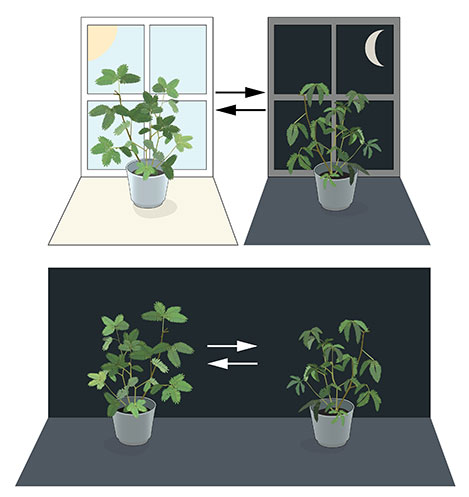
\includegraphics[width=0.5\textwidth,height=\textheight]{images/nobel-prize-outreach-ab-2017-de-mairan-experiment.jpg}

\legend{Source: Reproduction from \textcite{nobelprizeoutreachab}.}

}

\end{figure}%

Science has already demonstrated and described various biological
rhythms and their impacts on organisms. These rhythms can occur at
different levels, whether at a macro level, such as the menstrual cycle,
or even at a micro level, such as rhythms expressed within cells
\autocite{roenneberg2016}. Like many other biological phenomena, these
are complex systems present in all living beings, i.e., a emergence
created by a large number of connected and interecticve agents that
exhibit adaptive characteristics, all without the need of a central
control \autocite{boccara2010}. It is understood today that the
endogeneity of rhythms has provided organisms with an anticipatory
capacity, allowing them to organize resources and activities before they
are needed \autocite{marques2003}.

Despite the endogenous nature of these rhythms, they can still be
regulated by the external environment. Signals (cues) from the
environment that occur cyclically and have the ability to regulate
biological rhythmic expression are called zeitgebers (from the German
\emph{zeit}, meaning time, and \emph{geber}, meaning donor
\autocite{cambridgeuniversitypress}). These zeitgebers act as
synchronizers by entraining the phases of biological rhythms
\autocite{khalsa2003,kuhlman2018} (see
Figure~\ref{fig-chapter-1-kuhlman-2018-figure-2b}). Among the known
zeitgebers are, for example, meal timing and changes in environmental
temperature \autocite{aschoff1981,roenneberg2016}. However, the most
influential of them is the light-dark cycle. It is understood that the
day/night cycle, resulting from the rotation of the Earth, has provided
the vast majority of organisms with an oscillatory system with a
periodic duration of approximately 24 hours
\autocite{kuhlman2018,roenneberg2007}.

\begin{figure}[H]

\caption{\label{fig-chapter-1-kuhlman-2018-figure-2b}Illustration of a
circadian rhythm (output) whose phase is entrained in the presence of a
zeitgeber (input). The rectangles represent the light-dark cycle.}

\centering{

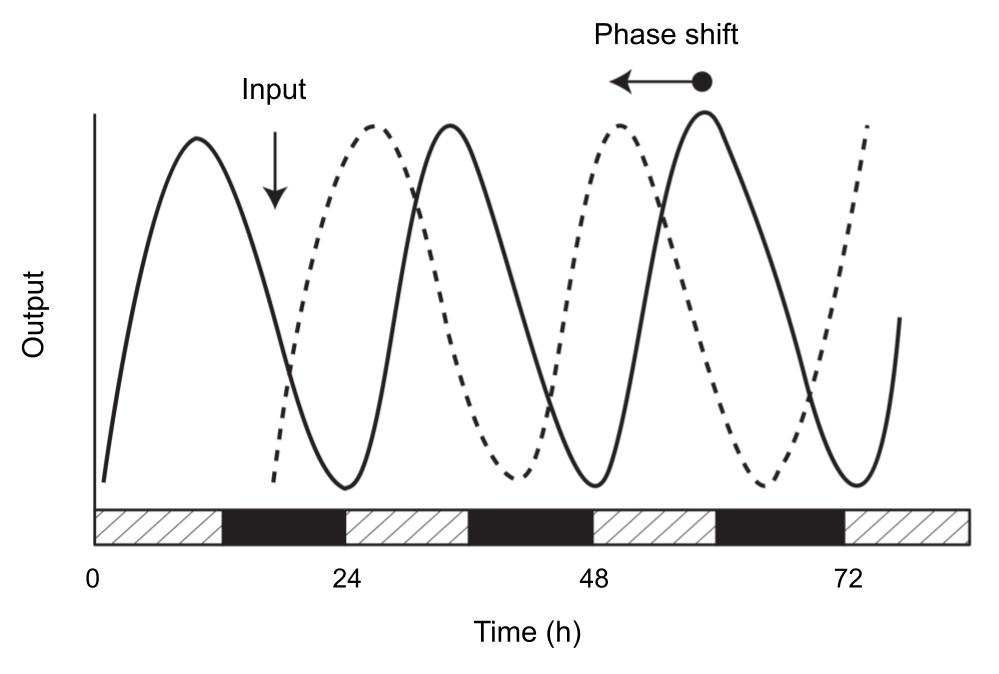
\includegraphics[width=0.75\textwidth,height=\textheight]{images/kuhlman-2018-figure-2b.jpg}

\legend{Source: Adapted from \textcite{kuhlman2018}.}

}

\end{figure}%

Naturally, the expression of this temporal organization varies from
organism to organism, even among members of the same species, whether
due to the different ways they are exposed to the environment or the
differences in the expression of endogenous rhythmicity, which, in turn,
results from gene expression \autocite{roenneberg2007a}. The interaction
between these two expressions, external and internal, of the environment
and genotype, generates a signature, an observable characteristic, which
is called a phenotype \autocite{frommlet2016}.

The various temporal characteristics of an organism can be linked to
different oscillatory periods. Among these are circadian phenotypes,
which refer to characteristics observed in rhythms with periods lasting
about a day \autocite{foster2005}. Another term used for these temporal
phenotypes, as the name suggest, is \emph{chronotype}
\autocite{ehret1974,pittendrigh1993}. This term is also often used to
differentiate phenotypes on a spectrum ranging from morningness to
eveningness \autocite{horne1976,roenneberg2019b}.

Sleep is a phenomenon that exhibits circadian expression. By observing
the sleep characteristics of individuals, it is possible to assess the
distribution of circadian phenotypes within the same population, thereby
investigating their covariates and other relevant associations
\autocite{roenneberg2003}. This is because sleep regulation is
understood as the result of the interaction between two processes: a
homeostatic process (referred to as the \(\text{S}\) process), which is
sleep-dependent and accumulates with sleep deprivation, and a circadian
process (referred to as the \(\text{C}\) process), whose expression can
be influenced by zeitgebers, such as the light-dark cycle
\autocite{borbely1982,borbely2016}
(Figure~\ref{fig-chapter-1-borbely-1982-figure-4} illustrates these two
process). Considering that the circadian rhythm (the \(\text{C}\)
process) is present in sleep, its characteristics can be estimated if
the \(\text{S}\) process can be controlled.

\begin{figure}[H]

\caption{\label{fig-chapter-1-borbely-1982-figure-4}Illustration of the
interaction of the \(\text{S}\) process and the \(\text{C}\) process in
sleep regulation. The figure depicts two scenarios: one without sleep
deprivation and another with sleep deprivation. The \(y\)-axis
represents the level of the process.}

\centering{

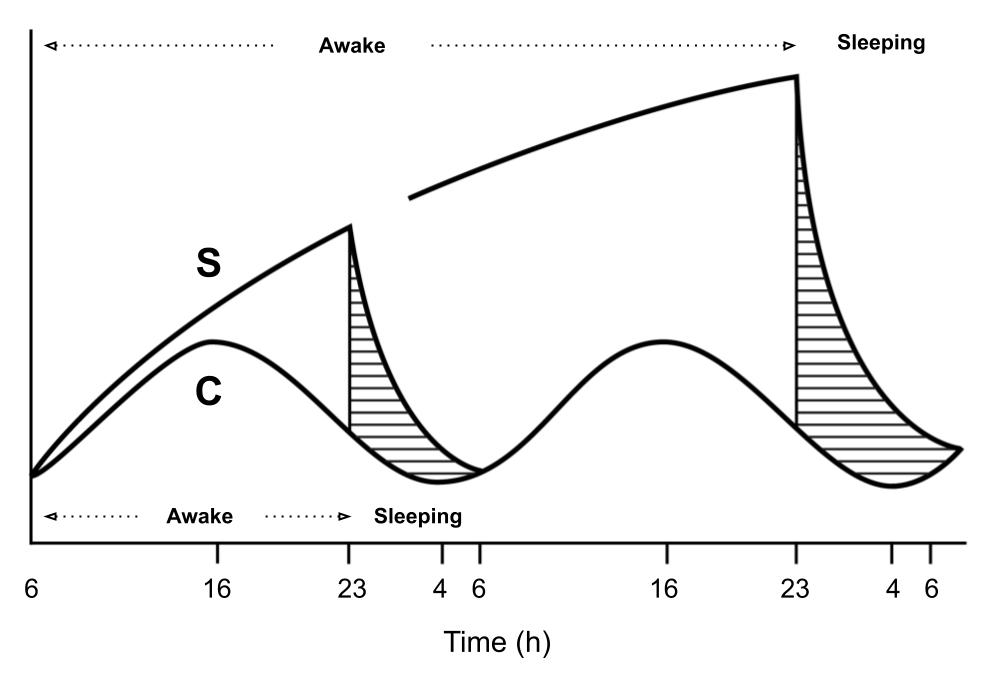
\includegraphics[width=0.75\textwidth,height=\textheight]{images/borbely-1982-figure-4.jpg}

\legend{Source: Adapted from \textcite{borbely1982}.}

}

\end{figure}%

Although many theories related to sleep and circadian rhythms are
well-established in science, it is still necessary to verify and test
them in larger samples to obtain a more accurate picture of the
mechanisms related to the ecology of sleep and chronotypes. This project
undertakes this commitment with the aim of investigating a hypothesis
that is still relatively untested but widely accepted in chronobiology,
which suggests that latitude is associated with the regulation of
circadian rhythms
\autocite{hut2013,leocadio-miguel2014,leocadio-miguel2017,pittendrigh1991,randler2008,randler2017,roenneberg2003}.

The latitude hypothesis is based on the idea that regions located at
latitudes close to the poles, on average, experience less annual
sunlight exposure compared to regions near the equator. Therefore, it is
deduced that regions near latitude 0° have a stronger solar zeitgeber,
which, according to chronobiology theories, should lead to a greater
propensity for the synchronization of circadian rhythms in these
populations with the light-dark cycle. This would reduce the amplitude
and diversity of circadian phenotypes found due to a lower influence of
individuals' characteristic endogenous periods. This would also give
these populations a morningness characteristic when compared to
populations living farther from the equator, where the opposite would
occur -- greater amplitude and diversity of circadian phenotypes and an
eveningness characteristic compared to populations living near latitude
0° \autocite{roenneberg2003}.

To achieve the mentioned objectives, this project will rely on a dataset
of the sleep-wake cycle expression of the Brazilian population,
consisting of \(120,265\) respondents covering all states of the
country. This dataset was collected in 2017 and is based on the Munich
ChronoType Questionnaire (MCTQ), a widely validated scale used to
measure chronotypes based on individuals' sleep-wake cycle expression in
the last four weeks \autocite{roenneberg2003,roenneberg2012a}.

\section{Thesis justification}\label{thesis-justification}

Mapping the sleep-wake cycles and circadian phenotypes of Brazilians can
contribute to the understanding of various phenomena related to sleep
and chronobiology, such as the relationship between latitude and the
regulation of circadian rhythms, the hypothesis tested by this thesis.
However, in addition to contributing to the validation of theories and
the advancement of scientific knowledge, the data, information, and
knowledge generated by this project will also serve the public interest
as a guide for public policies related to sleep and population health.
Scientific literature is filled with studies pointing to negative
associations with human health stemming from the disruption of
biological rhythms. These range from fatigue \autocite{tryon2004},
deficits in cognitive performance \autocite{dongen2003} ,
gastrointestinal problems \autocite{fido2008,morito2014,mortas2020},
mental disorders \autocite{jones2005,kalmbach2015,roh2012} and even
cancer \autocite{lie2006,papantoniou2015,schernhammer2001}.

This study will also produce the largest dataset of valid sleep-wake
cycle expression among Brazilians ever recorded. For comparison,
national epidemiological studies on sleep and circadian phenotypes such
as those by \textcite{drager2022} and \textcite{leocadio-miguel2017}
worked with samples of \(2,635\) and \(12,884\) individuals,
respectively. The sample of this project includes \(120,265\)
individuals in its raw state, covering all Brazilian states. Another
advantage of the sample is its cross-sectional nature, as \(98.173\%\)
of the data were collected during a single week (from October 15 to 21,
2017). This avoids potential distortions caused by seasonal effects.

\section{Thesis aims}\label{thesis-aims}

This project focuses on the ecology of sleep and circadian phenotypes
(chronotypes) with the aim of providing answers to the following
questions:

\begin{enumerate}
\def\labelenumi{\arabic{enumi}.}
\item
  How are the sleep-wake cycles and circadian phenotypes of the adult
  Brazilian population characterized?
\item
  Is latitude associated with the regulation of circadian rhythms in
  humans?
\end{enumerate}

The basic hypothesis to be tested is that populations residing near the
equator (latitude 0°) have, on average, a shorter/more morning-oriented
circadian phenotype compared to populations living near the Earth's
poles (H1)
\autocite{hut2013,leocadio-miguel2014,leocadio-miguel2017,pittendrigh1991,randler2008,randler2017,roenneberg2003}.

The primary objectives (PO) of the project are as follows:

\microskip

\begin{enumerate}
\def\labelenumi{\Alph{enumi})}
\item
  Quantitatively describe the expression of sleep-wake cycles and
  circadian phenotypes of the Brazilian adult population at the end of
  the year 2017 (pre-pandemic).
\item
  Investigate and model the presence/absence of a significant
  association and effect between decimal degrees of latitude
  (independent variable (IV)) and circadian phenotypes (dependent
  variable (DV)) of the Brazilian population.
\end{enumerate}

\microskip

To achieve the primary objectives, the following secondary objectives
(SO) have been outlined:

\microskip

\begin{enumerate}
\def\labelenumi{\roman{enumi})}
\item
  Conduct data cleaning, validation, and transformation processes on the
  obtained sample data.
\item
  Collect secondary data on geolocation and solarimetric models and
  cross-reference them with the primary data.
\item
  Develop algorithms for generating randomly sampled subsets adjusted to
  the proportions of the analyzed Brazilian regions, based on the latest
  Brazilian demographic census.
\item
  Develop algorithms and models to help with the processing of MCTQ data
  and to simulate the complexity of the entrainment phenomena.
\item
  Evaluate and discuss the presence/absence of significant differences
  in the values of the corrected mid-sleep on free days (MSFsc) (DV) ---
  a proxy for the expression of individuals' circadian phenotypes ---
  based on decimal degrees of latitude (IV), while controlling for known
  covariates such as respondents' gender and age.
\end{enumerate}

\section{Projects developed}\label{projects-developed}

In addition to the main investigation, which is center on testing the
latitude hypothesis, four additional projects/analyses were devised for
this thesis. Each project was organized into a separate chapter, with
the intention of crafting each chapter in a manner suitable for
submission to a scientific journal. This organizational approach was
influenced by the doctoral thesis of \textcite{reis2020}.

The first project involves a concise paper that delineates the
resemblance observed among Portuguese translations of the MCTQ (Munich
ChronoType Questionnaire) employed in scientific research. It's crucial
to emphasize that, although the MCTQ functions as a self-report scale
for assessing chronotypes, it primarily relies on objective temporal
metrics (e.g., local bedtime, sleep latency duration) rather than more
subjective factors such as perceived sleep quality. Essentially, it
functions as a sleep diary. Nevertheless, these translations can exhibit
noteworthy discrepancies. It's worth noting that the proper validation
of MCTQ in Portuguese was only achieved in 2020 through the efforts of
\textcite{reis2020}. The aim of this project is to assess the semantic
similarity among these translations using a natural language model (NLM)
known as Bidirectional Encoder Representations from Transformers (BERT),
developed by Google, and pretrained on the Portuguese language
\autocite{devlin2018,souza2020}. By leveraging these semantic
representation vectors, the translations will be evaluated based on
cosine similarity.

The second project is an R package comprising a suite of tools designed
for processing the MCTQ questionnaire. While it may appear to be a
straightforward questionnaire, the MCTQ necessitates a considerable
amount of date and time manipulation. This presents a challenge for many
scientists, as handling date and time data can be particularly tricky,
especially when dealing with extensive datasets. By creating a free,
open-source and peer-reviewed R package, it becomes possible to
standardize the analyses and enhance reproducibility for all research
related to the MCTQ. This R package \autocite{vartanian2023}has already
been developed and published on
\href{https://cran.r-project.org/web/packages/mctq/index.html}{CRAN}
(The Comprehensive R Archive Network) and
\href{https://github.com/ropensci/mctq}{GitHub}. It has been downloaded
more than \(6,000\) to this date, and underwent a peer review by the
\href{https://ropensci.org/}{rOpenSci Initiative}. Chapter 2 will serve
as a manuscript for a publication regarding the package in the
\href{https://www.jstatsoft.org/authors}{Journal of Statistical
Software}.

The third project is centered around the project's extensive MCTQ data
sample, representing the largest dataset collected within a single
country for this questionnaire thus far. This chapter serves as a
crucial step in fulfilling one of the thesis primary objectives, which
is to describe the sleep-wake cycle and circadian characteristics of the
Brazilian population. Achieving this goal entails rigorous data cleaning
and comprehensive data wrangling efforts. Furthermore, it functions as a
means to facilitate the utilization of this valuable sample in future
scientific research, while ensuring full compliance with ethical
requirements.

The fourth project involves a rule-based model focusing on entrainment
phenomena. Complex systems, such as biological rhythms, often exhibit
the challenge of being described or represented concisely, as noted by
David Krakauer (cited in \textcite{mitchell2013}). Rule-based or
agent-based models offer a means to simulate scenarios involving a
multitude of agents and interactions. Models of this nature, underpinned
by scientific theory-based rules, can provide valuable insights and
enhance our comprehension of the various manifestations of entrainment
phenomena within a population context. They offer an effective means to
understand the implications of theory and test them against real-world
data. An initial version of this package was developed as a Python
package and is currently accessible on
\href{https://entrainment.readthedocs.io/en/latest/index.html}{GitHub}
\autocite[see][]{vartanian2022}.

The fifth and final project is the test of the latitude hypothesis,
which serves as the primary investigation. It's important to note that
all the preceding projects converge into this one. The first project
focuses on validating the MCTQ translation used for data collection. The
second project involves the development of data processing tools. The
third project is responsible for the necessary data manipulation to
prepare it for analysis. The fourth project aims to offer valuable
insights and guidance for the upcoming tasks.

All of these projects are developed using secure, open-source tools and
adhere to the best international standards. They are designed to ensure
100\% reproducibility and are accompanied by extensive documentation.

\section{Related activities}\label{related-activities}

During the development of this thesis, several activities and results
have been accomplished. These activities are important to note, as they
demonstrate the path taken to arrive at this final document.

\subsection{Courses}\label{courses}

The following graduate courses from the University of São Paulo (USP)
were completed during the first year of the master's program.

\begin{itemize}
\tightlist
\item
  2022/2: \emph{SCX5000 - Mathematical and Computational Methods I} (10
  credits) (Concept: \textbf{C});
\item
  2022/2: \emph{SCX5002 - Complex Systems I} (10 credits) (Concept:
  \textbf{A});
\item
  2023/1: \emph{SCX5001 - Mathematical and Computational Methods II} (10
  credits) (Concept: \textbf{A});
\item
  2023/1: \emph{SCX5017 - Introduction to Data Science} (10 credits)
  (Concept: \textbf{A});
\item
  2023/1: \emph{EAH5001 - Pedagogic Preparation} (4 credits) (Concept:
  \textbf{A}).
\end{itemize}

Please note that the unfortunate \textbf{C} concept above happened in
the same semester when the author broke relations with his former
supervisor (\emph{Mario Pedrazzoli}).

44 discipline credits were completed by this thesis publication date. An
additional 12 special credits, related to an article publication (see
\textcite{viana-mendes2023}), were requested and approved by the
Graduate Program Coordination Commission (CCP) in accordance with
\href{https://leginf.usp.br/?resolucao=resolucao-copgr-no-7829-de-03-de-outubro-de-2019}{program
regulations}. In total, 56 credits were earned. A minimum of 50 credits
is required for the thesis defense.

\subsection{Teaching internship}\label{teaching-internship}

Scholarship students under the
\href{https://www.gov.br/capes/}{Coordination for the Improvement of
Higher Education Personnel (CAPES)} are required to participate in the
\href{www5.each.usp.br/pae/}{Teaching Improvement Program (PAE)}. This
internship is currently in progress and is scheduled to conclude in
December 2023.

The internship responsibilities entail serving as an Assistant Professor
for the undergraduate course \emph{ACH0042 - Problem-Based Learning II}
at USP. A comprehensive teaching plan \autocite{vartanian2023e} was
formulated during enrollment in the aforementioned graduate course
\emph{EAH5001}, and it is accessible through the following link.

\smallskip

\noindent Vartanian, D., Bernardes, M. E. M., \& Rodrigues Neto, C.
(2023). \emph{Plano de ensino: ACH0042 - Resolução de Problemas II}.
\url{https://doi.org/10.13140/RG.2.2.33335.50086}

\subsection{Publications}\label{publications}

The following article \autocite{viana-mendes2023} was published during
the development of this thesis.

\smallskip

\noindent Viana-Mendes, J., Benedito-Silva, A. A., Andrade, M. A. M.,
\textbf{Vartanian, D.}, Gonçalves, B. da S. B., Cipolla-Neto, J., \&
Pedrazzoli, M. (2023). Actigraphic characterization of sleep and
circadian phenotypes of PER3 gene VNTR genotypes. \emph{Chronobiology
International}. \url{https://doi.org/10.1080/07420528.2023.2256858}

\subsection{Translations}\label{translations}

As a member and package developer of the
\href{https://ropensci.org/}{rOpenSci Initiative} (based in Berkeley,
CA), the author is actively contributing to the
\href{https://github.com/ropensci/dev_guide/pull/717}{ongoing
translation} of the \href{https://devguide.ropensci.org/}{rOpenSci
Developer Guide} into Portuguese. The aim is to create a more inclusive
environment for individuals in Brazil and other Portuguese-speaking
countries when developing for the \href{https://www.r-project.org/}{R
programming language}.

This endeavor is linked to the thesis, as the author's membership in
rOpenSci began with the creation of the
\href{https://docs.ropensci.org/mctq/}{\{mctq\} R package} (listed
below).

\subsection{Conferences}\label{conferences}

An abstract pertaining to the primary investigation was published and
presented on a poster at the
\href{https://espca.fapesp.br/school/sao_paulo_school_of_advanced_science_on_ecology_of_human_sleep_and_biological_rhythms/101/}{Sao
Paulo School of Advanced Science on Ecology of Human Sleep and
Biological Rhythms} organized by the \href{https://fapesp.br/en}{São
Paulo Research Foundation (FAPESP)}. This international school hosted
100 participants, including students and young researchers, with a
diverse representation of 50 individuals from various states within
Brazil and an additional 50 from international backgrounds. The event
took place from November 16, 2022, to November 26, 2022.

\smallskip

\noindent Vartanian, D., \& Pedrazzoli, M. (2022). \emph{Ecology of
sleep and circadian phenotypes of the Brazilian population}
{[}Poster{]}. São Paulo Research Foundation; São Paulo School of
Advanced Science on Ecology of Human Sleep and Biological Rhythms.
\url{https://doi.org/10.13140/RG.2.2.25343.07840}

\smallskip

In the same semester (2022/2), the author also participated in USP's
International Symposium on Scientific and Technological Initiation
(SIICUSP) as both an examiner and a participant. As a participant, the
author presented a research abstract related to the
\href{https://github.com/giperbio/actverse}{\{actverse\} R package} for
actigraphy data analysis, as detailed in \textcite{matias2022} and
\textcite{vartanian2022b}. This project was conceived and developed by
the author of this thesis and involved collaboration with two
undergraduate students. Notably, this project achieved recognition,
securing 2nd place in the category of \emph{Earth and Exact Sciences}.

\subsection{Research compendia}\label{research-compendia}

This thesis, along with all the accompanying research, is structured and
organized within the research compendium provided below.

\smallskip

\noindent Vartanian, D. (2023). \emph{Ecology of sleep and circadian
phenotypes of the Brazilian population} {[}Research compendium{]}.
\url{https://danielvartan.github.io/mastersthesis/}

\subsection{Data plans}\label{data-plans}

This research has also produced and published the following open data
model and data plan.

\smallskip

\noindent Vartanian, D. (2023). \emph{Ecology of sleep and circadian
phenotypes of the Brazilian population} {[}Data Management Plan{]}.
DMPHub. \url{https://doi.org/10.48321/D1DW8P}

\subsection{Softwares}\label{softwares}

The following R packages, \href{https://quarto.org/}{Quarto} format
(being used to write this thesis), and Python package were developed in
relation with this thesis.

\smallskip

\noindent Vartanian, D. (2022). \emph{\{entrainment\}: a rule-based
model of the 24h light/dark cycle entrainment phenomenon} {[}Software,
Python Package{]}. \url{https://github.com/danielvartan/entrainment}

\microskip

\noindent Vartanian, D. (2023). \emph{\{mctq\}: tools to process the
Munich ChronoType Questionnaire (MCTQ)} {[}Software, R Package
v0.3.2{]}. \url{https://docs.ropensci.org/mctq/}

\microskip

\noindent Vartanian, D. (2023). \emph{\{lockr\}: easily encrypt/decrypt
files} {[}Software, R package v0.3.0{]}.
\url{https://github.com/danielvartan/lockr}

\microskip

\noindent Vartanian, D. (2023). \emph{\{lubritime\}: an extension for
the lubridate package} {[}Software, R package{]}.
\url{https://github.com/danielvartan/lubritime}

\microskip

\noindent Vartanian, D. (2023). \emph{\{abnt\}: Quarto format for ABNT
theses and dissertations} {[}Software, LaTeX/R format, v0.3.0{]}.
\url{https://github.com/danielvartan/abnt/}

\subsection{Other projects}\label{other-projects}

The author is also currently working on the development of the project
below.

\smallskip

\noindent Sales, A. R. V., Vartanian, D., Andrade, M. A. M., Pedrazzoli,
M. (2023). \emph{Associations between the duration and quality of sleep
in third-trimester pregnant women and the duration of labor} {[}PhD
project, University of Sao Paulo{]}. \url{https://bit.ly/3S6O0MB}

\bookmarksetup{startatroot}

\chapter{\texorpdfstring{Similarities between different versions of the
MCTQ\textsuperscript{PT}}{Similarities between different versions of the MCTQPT}}\label{similarities-between-different-versions-of-the-mctqpt}

\begin{tcolorbox}[enhanced jigsaw, colframe=quarto-callout-important-color-frame, coltitle=black, opacityback=0, left=2mm, opacitybacktitle=0.6, rightrule=.15mm, leftrule=.75mm, colbacktitle=quarto-callout-important-color!10!white, titlerule=0mm, title=\textcolor{quarto-callout-important-color}{\faExclamation}\hspace{0.5em}{Important}, colback=white, breakable, bottomtitle=1mm, toptitle=1mm, arc=.35mm, bottomrule=.15mm, toprule=.15mm]

You are reading the work-in-progress of this thesis.

\microskip

This chapter is currently a dumping ground for ideas, and I don't
recommend reading it.

\end{tcolorbox}

\begin{tcolorbox}[enhanced jigsaw, colframe=quarto-callout-note-color-frame, coltitle=black, opacityback=0, left=2mm, opacitybacktitle=0.6, rightrule=.15mm, leftrule=.75mm, colbacktitle=quarto-callout-note-color!10!white, titlerule=0mm, title=\textcolor{quarto-callout-note-color}{\faInfo}\hspace{0.5em}{Target journal}, colback=white, breakable, bottomtitle=1mm, toptitle=1mm, arc=.35mm, bottomrule=.15mm, toprule=.15mm]

\begin{enumerate}
\def\labelenumi{\arabic{enumi}.}
\tightlist
\item
  \href{https://www.tandfonline.com/action/authorSubmission?show=instructions&journalCode=icbi20}{Chronobiology
  International} (\href{https://jcr.clarivate.com/jcr/}{IF 2022:
  2.8/JCR} \textbar{}
  \href{https://sucupira.capes.gov.br/sucupira/public/consultas/coleta/veiculoPublicacaoQualis/listaConsultaGeralPeriodicos.jsf}{A1/2017-2020}).
\item
  \href{https://journals.sagepub.com/author-instructions/JBR}{Journal of
  Biological Rhythms} (\href{https://jcr.clarivate.com/jcr/}{IF 2022:
  3.5/JCR} \textbar{}
  \href{https://sucupira.capes.gov.br/sucupira/public/consultas/coleta/veiculoPublicacaoQualis/listaConsultaGeralPeriodicos.jsf}{A2/2017-2020}).
\end{enumerate}

\end{tcolorbox}

\begin{tcolorbox}[enhanced jigsaw, colframe=quarto-callout-note-color-frame, coltitle=black, opacityback=0, left=2mm, opacitybacktitle=0.6, rightrule=.15mm, leftrule=.75mm, colbacktitle=quarto-callout-note-color!10!white, titlerule=0mm, title=\textcolor{quarto-callout-note-color}{\faInfo}\hspace{0.5em}{Note}, colback=white, breakable, bottomtitle=1mm, toptitle=1mm, arc=.35mm, bottomrule=.15mm, toprule=.15mm]

The following study was performed by Daniel Vartanian (DV) and Camilo
Rodrigues Neto (CR).

\microskip

\textbf{DV} and \textbf{CR} contributed to the study's design.
\textbf{DV} implemented the study, performed the statistical analysis,
and authored the manuscript. All authors participated in discussions
about the results and contributed to the final manuscript revision.

\microskip

\emph{Future reference}: Vartanian, D., \& Rodrigues Neto, C. (2024).
Similarities between different versions of the MCTQ\textsuperscript{PT}.
\emph{Chronobiology International}.

\end{tcolorbox}

\bookmarksetup{startatroot}

\chapter{The \{mctq\} R package}\label{the-mctq-r-package}

\begin{tcolorbox}[enhanced jigsaw, colframe=quarto-callout-important-color-frame, coltitle=black, opacityback=0, left=2mm, opacitybacktitle=0.6, rightrule=.15mm, leftrule=.75mm, colbacktitle=quarto-callout-important-color!10!white, titlerule=0mm, title=\textcolor{quarto-callout-important-color}{\faExclamation}\hspace{0.5em}{Important}, colback=white, breakable, bottomtitle=1mm, toptitle=1mm, arc=.35mm, bottomrule=.15mm, toprule=.15mm]

You are reading the work-in-progress of this thesis.

\microskip

This chapter is currently a dumping ground for ideas, and I don't
recommend reading it.

\end{tcolorbox}

\begin{tcolorbox}[enhanced jigsaw, colframe=quarto-callout-note-color-frame, coltitle=black, opacityback=0, left=2mm, opacitybacktitle=0.6, rightrule=.15mm, leftrule=.75mm, colbacktitle=quarto-callout-note-color!10!white, titlerule=0mm, title=\textcolor{quarto-callout-note-color}{\faInfo}\hspace{0.5em}{Target journal}, colback=white, breakable, bottomtitle=1mm, toptitle=1mm, arc=.35mm, bottomrule=.15mm, toprule=.15mm]

\begin{enumerate}
\def\labelenumi{\arabic{enumi}.}
\tightlist
\item
  \href{https://www.jstatsoft.org/authors}{Journal of Statistical
  Software} (\href{https://jcr.clarivate.com/jcr/}{IF 2022: 5.8/JCR}
  \textbar{}
  \href{https://sucupira.capes.gov.br/sucupira/public/consultas/coleta/veiculoPublicacaoQualis/listaConsultaGeralPeriodicos.jsf}{A1/2017-2020}).
\item
  \href{https://joss.readthedocs.io/en/latest/submitting.html}{Journal
  of Open Source Software}
  (\href{https://sucupira.capes.gov.br/sucupira/public/consultas/coleta/veiculoPublicacaoQualis/listaConsultaGeralPeriodicos.jsf}{B1/2017-2020}).
\end{enumerate}

\end{tcolorbox}

\begin{tcolorbox}[enhanced jigsaw, colframe=quarto-callout-note-color-frame, coltitle=black, opacityback=0, left=2mm, opacitybacktitle=0.6, rightrule=.15mm, leftrule=.75mm, colbacktitle=quarto-callout-note-color!10!white, titlerule=0mm, title=\textcolor{quarto-callout-note-color}{\faInfo}\hspace{0.5em}{Note}, colback=white, breakable, bottomtitle=1mm, toptitle=1mm, arc=.35mm, bottomrule=.15mm, toprule=.15mm]

The following study was conducted by Daniel Vartanian (\textbf{DV}), Ana
Amélia Benedito-Silva (\textbf{AA}), Mario Pedrazzoli (\textbf{MP}), and
Camilo Rodrigues Neto (\textbf{CR}).

\microskip

\textbf{DV} contributed to the conception, design, coding, and
implementation of the software. \textbf{AA}, \textbf{MP}, and
\textbf{CR} served as scientific advisors and reviewers. \textbf{DV}
authored the manuscript. All authors discussed the results and revised
the final manuscript.

\microskip

\emph{Future reference}: Vartanian, D., Benedito-Silva, A. A.,
Pedrazzoli, M., \& Rodrigues Neto, C. (2024). \{mctq\}: tools to process
the Munich ChronoType Questionnaire (MCTQ). \emph{Journal of Statistical
Software}.

\end{tcolorbox}

\bookmarksetup{startatroot}

\chapter{Ecology of sleep and circadian phenotypes of the brazilian
population}\label{ecology-of-sleep-and-circadian-phenotypes-of-the-brazilian-population}

\begin{tcolorbox}[enhanced jigsaw, colframe=quarto-callout-important-color-frame, coltitle=black, opacityback=0, left=2mm, opacitybacktitle=0.6, rightrule=.15mm, leftrule=.75mm, colbacktitle=quarto-callout-important-color!10!white, titlerule=0mm, title=\textcolor{quarto-callout-important-color}{\faExclamation}\hspace{0.5em}{Important}, colback=white, breakable, bottomtitle=1mm, toptitle=1mm, arc=.35mm, bottomrule=.15mm, toprule=.15mm]

You are reading the work-in-progress of this thesis.

\microskip

This chapter is currently a dumping ground for ideas, and I don't
recommend reading it.

\end{tcolorbox}

\begin{tcolorbox}[enhanced jigsaw, colframe=quarto-callout-note-color-frame, coltitle=black, opacityback=0, left=2mm, opacitybacktitle=0.6, rightrule=.15mm, leftrule=.75mm, colbacktitle=quarto-callout-note-color!10!white, titlerule=0mm, title=\textcolor{quarto-callout-note-color}{\faInfo}\hspace{0.5em}{Target journal}, colback=white, breakable, bottomtitle=1mm, toptitle=1mm, arc=.35mm, bottomrule=.15mm, toprule=.15mm]

\begin{enumerate}
\def\labelenumi{\arabic{enumi}.}
\tightlist
\item
  \href{https://www.tandfonline.com/action/authorSubmission?show=instructions&journalCode=icbi20}{Chronobiology
  International} (\href{https://jcr.clarivate.com/jcr/}{IF 2022:
  2.8/JCR} \textbar{}
  \href{https://sucupira.capes.gov.br/sucupira/public/consultas/coleta/veiculoPublicacaoQualis/listaConsultaGeralPeriodicos.jsf}{A1/2017-2020}).
\item
  \href{https://journals.sagepub.com/author-instructions/JBR}{Journal of
  Biological Rhythms} (\href{https://jcr.clarivate.com/jcr/}{IF 2022:
  3.5/JCR} \textbar{}
  \href{https://sucupira.capes.gov.br/sucupira/public/consultas/coleta/veiculoPublicacaoQualis/listaConsultaGeralPeriodicos.jsf}{A2/2017-2020}).
\end{enumerate}

\end{tcolorbox}

\begin{tcolorbox}[enhanced jigsaw, colframe=quarto-callout-note-color-frame, coltitle=black, opacityback=0, left=2mm, opacitybacktitle=0.6, rightrule=.15mm, leftrule=.75mm, colbacktitle=quarto-callout-note-color!10!white, titlerule=0mm, title=\textcolor{quarto-callout-note-color}{\faInfo}\hspace{0.5em}{Note}, colback=white, breakable, bottomtitle=1mm, toptitle=1mm, arc=.35mm, bottomrule=.15mm, toprule=.15mm]

The following study was conducted by Daniel Vartanian (DV), Mario
Pedrazzoli (MP), and Camilo Rodrigues Neto (CR).

\microskip

\textbf{DV} conceived the study, contributed with the design,
implementation, statistical analysis and authored the manuscript.
\textbf{CR} contributed as a science adviser and reviewer. \textbf{DV}
and \textbf{MP} were responsible for data collection. All authors
actively participated in discussions regarding the results and
contributed to the final manuscript.

\microskip

\emph{Future reference}: Vartanian, D., Pedrazzoli, M., \& Rodrigues
Neto, C. (2024). Ecology of sleep and circadian phenotypes of the
Brazilian population. \emph{Chronobiology International}.

\end{tcolorbox}

\bookmarksetup{startatroot}

\chapter{Rule-based model of the 24h light/dark entrainment
phenomenon}\label{rule-based-model-of-the-24h-lightdark-entrainment-phenomenon}

\begin{tcolorbox}[enhanced jigsaw, colframe=quarto-callout-important-color-frame, coltitle=black, opacityback=0, left=2mm, opacitybacktitle=0.6, rightrule=.15mm, leftrule=.75mm, colbacktitle=quarto-callout-important-color!10!white, titlerule=0mm, title=\textcolor{quarto-callout-important-color}{\faExclamation}\hspace{0.5em}{Important}, colback=white, breakable, bottomtitle=1mm, toptitle=1mm, arc=.35mm, bottomrule=.15mm, toprule=.15mm]

You are reading the work-in-progress of this thesis.

\microskip

This chapter is currently a dumping ground for ideas, and I don't
recommend reading it.

\end{tcolorbox}

\begin{tcolorbox}[enhanced jigsaw, colframe=quarto-callout-note-color-frame, coltitle=black, opacityback=0, left=2mm, opacitybacktitle=0.6, rightrule=.15mm, leftrule=.75mm, colbacktitle=quarto-callout-note-color!10!white, titlerule=0mm, title=\textcolor{quarto-callout-note-color}{\faInfo}\hspace{0.5em}{Target journal}, colback=white, breakable, bottomtitle=1mm, toptitle=1mm, arc=.35mm, bottomrule=.15mm, toprule=.15mm]

\begin{enumerate}
\def\labelenumi{\arabic{enumi}.}
\tightlist
\item
  \href{https://joss.readthedocs.io/en/latest/submitting.html}{Journal
  of Open Source Software}
  (\href{https://sucupira.capes.gov.br/sucupira/public/consultas/coleta/veiculoPublicacaoQualis/listaConsultaGeralPeriodicos.jsf}{B1/2017-2020}).
\end{enumerate}

\end{tcolorbox}

\begin{tcolorbox}[enhanced jigsaw, colframe=quarto-callout-note-color-frame, coltitle=black, opacityback=0, left=2mm, opacitybacktitle=0.6, rightrule=.15mm, leftrule=.75mm, colbacktitle=quarto-callout-note-color!10!white, titlerule=0mm, title=\textcolor{quarto-callout-note-color}{\faInfo}\hspace{0.5em}{Note}, colback=white, breakable, bottomtitle=1mm, toptitle=1mm, arc=.35mm, bottomrule=.15mm, toprule=.15mm]

The following study was conducted by Daniel Vartanian (DV) and Camilo
Rodrigues Neto (CR).

\microskip

\textbf{DV} was responsible for the design and software implementation.
\textbf{CR} contributed as a science adviser and reviewer. \textbf{DV}
wrote the manuscript. All authors discussed the results and revised the
final manuscript.

\microskip

\emph{Future reference}: Vartanian, D, \& Rodrigues Neto, C. (2024).
\{entrainment\}: a rule-based model of the 24h light/dark cycle
entrainment phenomenon. \emph{Journal of Open Source}.

\end{tcolorbox}

\bookmarksetup{startatroot}

\chapter{A biological approach for the latitudinal cline of the
chronotype}\label{a-biological-approach-for-the-latitudinal-cline-of-the-chronotype}

\begin{tcolorbox}[enhanced jigsaw, colframe=quarto-callout-note-color-frame, coltitle=black, opacityback=0, left=2mm, opacitybacktitle=0.6, rightrule=.15mm, leftrule=.75mm, colbacktitle=quarto-callout-note-color!10!white, titlerule=0mm, title=\textcolor{quarto-callout-note-color}{\faInfo}\hspace{0.5em}{Note}, colback=white, breakable, bottomtitle=1mm, toptitle=1mm, arc=.35mm, bottomrule=.15mm, toprule=.15mm]

You are reading the work-in-progress of this thesis.

\microskip

This chapter should be readable but is currently undergoing final
polishing.

\end{tcolorbox}

\begin{tcolorbox}[enhanced jigsaw, colframe=quarto-callout-warning-color-frame, coltitle=black, opacityback=0, left=2mm, opacitybacktitle=0.6, rightrule=.15mm, leftrule=.75mm, colbacktitle=quarto-callout-warning-color!10!white, titlerule=0mm, title=\textcolor{quarto-callout-warning-color}{\faExclamationTriangle}\hspace{0.5em}{Warning}, colback=white, breakable, bottomtitle=1mm, toptitle=1mm, arc=.35mm, bottomrule=.15mm, toprule=.15mm]

The results shown here are \textbf{preliminary}, so please take them
with a grain of salt.

\microskip

The data has not yet been fully cleaned, balanced, and cross-referenced
with the secondary databases. Think of these results as a low-resolution
preview of the final results. The step-by-step analysis can be seen in
the appendices section.

\end{tcolorbox}

\begin{tcolorbox}[enhanced jigsaw, colframe=quarto-callout-note-color-frame, coltitle=black, opacityback=0, left=2mm, opacitybacktitle=0.6, rightrule=.15mm, leftrule=.75mm, colbacktitle=quarto-callout-note-color!10!white, titlerule=0mm, title=\textcolor{quarto-callout-note-color}{\faInfo}\hspace{0.5em}{Target journal}, colback=white, breakable, bottomtitle=1mm, toptitle=1mm, arc=.35mm, bottomrule=.15mm, toprule=.15mm]

\begin{enumerate}
\def\labelenumi{\arabic{enumi}.}
\tightlist
\item
  \href{https://www.nature.com/srep/author-instructions}{Scientific
  Reports} (\href{https://jcr.clarivate.com/jcr/}{IF 2022: 4.6/JCR}
  \textbar{}
  \href{https://sucupira.capes.gov.br/sucupira/public/consultas/coleta/veiculoPublicacaoQualis/listaConsultaGeralPeriodicos.jsf}{A1/2017-2020}).
\end{enumerate}

\end{tcolorbox}

\begin{tcolorbox}[enhanced jigsaw, colframe=quarto-callout-note-color-frame, coltitle=black, opacityback=0, left=2mm, opacitybacktitle=0.6, rightrule=.15mm, leftrule=.75mm, colbacktitle=quarto-callout-note-color!10!white, titlerule=0mm, title=\textcolor{quarto-callout-note-color}{\faInfo}\hspace{0.5em}{Note}, colback=white, breakable, bottomtitle=1mm, toptitle=1mm, arc=.35mm, bottomrule=.15mm, toprule=.15mm]

The following study was performed by Daniel Vartanian (DV), Mario
Pedrazzoli (MP) and Camilo Rodrigues Neto (CR).

\microskip

\textbf{DV} contributed to the design and implementation of the study.
\textbf{DV} and \textbf{MP} collected the data. \textbf{DV} and
\textbf{CR} performed the statistical analysis. \textbf{DV} wrote the
manuscript. All authors discussed the results and revised the final
manuscript.

\microskip

\emph{Future reference}: Vartanian, D., Pedrazzoli, M., \& Rodrigues
Neto, C. (2024). A biological approach for the latitudinal cline of the
chronotype. \emph{Scientific Reports}.

\end{tcolorbox}

\noindent \textbf{Chronotypes are temporal phenotypes
\autocite{ehret1974,pittendrigh1993}. Observable traits, like weight and
eye color. Our current understanding of these traits is that they are
linked to our environment and are the result of evolution pressures for
creating an inner temporal organization
\autocite{aschoff1989,paranjpe2005}, a way that organisms found to
anticipate events. Having such an important function in nature, these
internal rhythms need to be closely aligned with environmental changes.
The agents that shift these oscillations towards the environment are
called zeitgebers and the shift phenomenon is called entrainment
\autocite{roenneberg2003a,roenneberg2010}. The main zeitgeber for humans
is light exposure, particularly the light of the sun
\autocite{khalsa2003,minors1991,roenneberg2007a}. Considering the major
role of light on entrainment, several studies hypothesized that the
latitude shift of the sun could influence or even define the chronotypes
of different populations
\autocite{horzum2015,hut2013,leocadio-miguel2017,leocadio-miguel2014,pittendrigh1991,randler2017}.
For example, populations that live close to the equator would be, on
average, more entrained to the light-dark cycle and have morning-leaning
characteristics. Here we test this hypothesis using a biological
measure, the chronotype state, provided by the Munich ChronoType
Questionnaire \autocite{roenneberg2003}. We tested the latitude
hypothesis on a sample with \(76,744\) subjects living in different
latitudes in Brazil. Our results show that, even with a wide, big, and
aligned sample, the latitude is associated only with negligible effect
sizes. The entrainment phenomenon appears to be much more complex than
previously imagined, opening new questions and contradictions that need
to be further investigated.}

\section{Main text}\label{main-text}

\subsection{Introduction}\label{introduction-1}

Humans can differ from one another in many ways. These observable
traits, like hair color or height, are called phenotypes and are also
presented in the way that our body functions.

A chronotype is a temporal phenotype
\autocite{ehret1974,pittendrigh1993}. This word is usually used to refer
to endogenous circadian rhythms, i.e., rhythms which periods that are
close to a day or 24 hours (\emph{circa diem}). The current body of
knowledge of Chronobiology, the science that studies biological rhythms,
indicates that the evolution of these internal oscillators is linked to
our oscillatory environment, like the day and night cycle, which, along
with our evolution, created environmental pressures for the development
of a temporal organization \autocite{aschoff1989,paranjpe2005}. A way in
which an organism could predict events and better manage its needs, like
storing food for the winter.

A temporal system wouldn't be of much use if it could not follow
environmental changes. To those environmental signals that can regulate
the biological rhythms are given the name zeitgeber (from the German
Zeit, time, and Geber, giver). These zeitgebers produce inputs in our
bodies that can shift and align those rhythms. This phenomenon is called
entrainment \autocite{roenneberg2003a,roenneberg2010}.

The main zeitgeber known today is the light, particularly the sun's
light \autocite{khalsa2003,minors1991,roenneberg2007a}. Considering its
influence in entraining the biological temporal system, several studies
hypothesize that the latitudinal shift of the sun, related to the
earth's axis, would produce, on average, different temporal traits in
populations that live close to the equator line when compared to
populations that live close to the planet's poles
\autocite{horzum2015,hut2013,leocadio-miguel2017,leocadio-miguel2014,pittendrigh1991,randler2017}.
That is because the latter ones would have greater oscillations in sun
activity and an overall weak solar zeitgeber. This is the latitude
hypothesis, that can also appear as an environmental hypothesis of
circadian rhythm regulation.

Recently there have been attempts to test the latitude hypothesis in
different settings, but, at least in humans, none of them have been
successful in seeing a significant effect size related to the
latitudinal cline. Some of these approaches worked with secondary data
and with small samples. One of the most serious attempts of testing this
hypothesis was made by Leocadio-Miguel et al.
\autocite*{leocadio-miguel2017} in 2017. They measured the chronotype of
\(12,884\) Brazillian subjects on a wide latitudinal spectrum using the
Morningness--Eveningness Questionnaire (MEQ). Their results showed a
negligible effect size. One possible reason for this is that the MEQ
measures psychological traits and not biological states
\autocite{roenneberg2019}, i.e., the circadian oscillation itself,
therefore, it's not the best way to answer the question
\autocite{leocadio-miguel2014}.

This article brings a novel attempt to test the latitude hypothesis,
using, this time, a biological approach provided by the Munich
ChronoType Questionnaire (MCTQ) \autocite{roenneberg2003}. Furthermore,
the test was carried out on the biggest chronotype sample ever collected
in a same country. A sample made of \(76,744\) subjects, all living in
the same timezone in Brazil, with only one week of difference between
questionnaire responses.

\subsection{Results}\label{results}

The local time of the midpoint between sleep onset and sleep end on
work-free days (\(\text{MSF}_{\text{sc}}\)), MCTQ proxy for measuring
the chronotype, had an overall mean of \(\text{04:28:35}\). The
distribution curve is shown in
Figure~\ref{fig-chapter-6-chronotype-distribution}.

That's the midsleep point of Brazilian subjects with an
intermediate/average chronotype. One can imagine, following the 7-9h
sleep recommendation for healthy adults of the American Academy of Sleep
Medicine (AASM) \autocite{watson2015}, that this average person would,
if he/she had no social obligations, typically wake up at about
\(\text{08:28:35}\).

\begin{Shaded}
\begin{Highlighting}[numbers=left,,]
\FunctionTok{source}\NormalTok{(here}\SpecialCharTok{::}\FunctionTok{here}\NormalTok{(}\StringTok{"R/utils.R"}\NormalTok{))}

\NormalTok{utc\_minus\_3\_states }\OtherTok{\textless{}{-}} \FunctionTok{c}\NormalTok{(}
  \StringTok{"Amapá"}\NormalTok{, }\StringTok{"Pará"}\NormalTok{, }\StringTok{"Maranhão"}\NormalTok{, }\StringTok{"Tocantins"}\NormalTok{, }\StringTok{"Piauí"}\NormalTok{, }\StringTok{"Ceará"}\NormalTok{,}
  \StringTok{"Rio Grande do Norte"}\NormalTok{, }\StringTok{"Paraíba"}\NormalTok{, }\StringTok{"Pernambuco"}\NormalTok{, }\StringTok{"Alagoas"}\NormalTok{, }\StringTok{"Sergipe"}\NormalTok{,}
  \StringTok{"Bahia"}\NormalTok{, }\StringTok{"Distrito Federal"}\NormalTok{, }\StringTok{"Goiás"}\NormalTok{, }\StringTok{"Minas Gerais"}\NormalTok{, }\StringTok{"Espírito Santo"}\NormalTok{,}
  \StringTok{"Rio de Janeiro"}\NormalTok{, }\StringTok{"São Paulo"}\NormalTok{, }\StringTok{"Paraná"}\NormalTok{, }\StringTok{"Santa Catarina"}\NormalTok{,}
  \StringTok{"Rio Grande do Sul"}
\NormalTok{)}

\NormalTok{data }\OtherTok{\textless{}{-}} 
\NormalTok{  targets}\SpecialCharTok{::}\FunctionTok{tar\_read}\NormalTok{(}\StringTok{"geocoded\_data"}\NormalTok{, }\AttributeTok{store =}\NormalTok{ here}\SpecialCharTok{::}\FunctionTok{here}\NormalTok{(}\StringTok{"\_targets"}\NormalTok{)) }\SpecialCharTok{|\textgreater{}}
\NormalTok{  dplyr}\SpecialCharTok{::}\FunctionTok{filter}\NormalTok{(state }\SpecialCharTok{\%in\%}\NormalTok{ utc\_minus\_3\_states) }\SpecialCharTok{|\textgreater{}}
\NormalTok{  dplyr}\SpecialCharTok{::}\FunctionTok{select}\NormalTok{(msf\_sc, age, sex, state, latitude, longitude) }\SpecialCharTok{|\textgreater{}}
\NormalTok{  tidyr}\SpecialCharTok{::}\FunctionTok{drop\_na}\NormalTok{(msf\_sc, age, sex, latitude)}
\end{Highlighting}
\end{Shaded}

\begin{Shaded}
\begin{Highlighting}[numbers=left,,]
\FunctionTok{source}\NormalTok{(here}\SpecialCharTok{::}\FunctionTok{here}\NormalTok{(}\StringTok{"R/plot\_chronotype.R"}\NormalTok{))}

\NormalTok{data }\SpecialCharTok{|\textgreater{}} 
  \FunctionTok{plot\_chronotype}\NormalTok{(}
    \AttributeTok{col =} \StringTok{"msf\_sc"}\NormalTok{, }
    \AttributeTok{x\_lab =} \StringTok{"Frequency (\%)"}\NormalTok{,}
    \AttributeTok{y\_lab =}\NormalTok{ latex2exp}\SpecialCharTok{::}\FunctionTok{TeX}\NormalTok{(}\StringTok{"Local time ($MSF\_\{sc\}$)"}\NormalTok{),}
    \AttributeTok{col\_width =} \FloatTok{0.8}\NormalTok{,}
    \AttributeTok{col\_border =} \FloatTok{0.6}\NormalTok{,}
    \AttributeTok{text\_size =}\NormalTok{ env\_vars}\SpecialCharTok{$}\NormalTok{base\_size,}
    \AttributeTok{chronotype\_cuts =} \ConstantTok{FALSE}\NormalTok{,}
    \AttributeTok{legend\_position =} \StringTok{"right"}
\NormalTok{  )}
\end{Highlighting}
\end{Shaded}

\begin{figure}[H]

\caption{\label{fig-chapter-6-chronotype-distribution}Distribution of
the local time of the midpoint between sleep onset and sleep end on
work-free days (\(\text{MSF}_{\text{sc}}\)), MCTQ proxy for measuring
the chronotype. The categorical cuts follow a quantile approach going
from extremely early (\(0 |- 0.11\)) to the extremely late
(\(0.88 - 1\)).}

\centering{

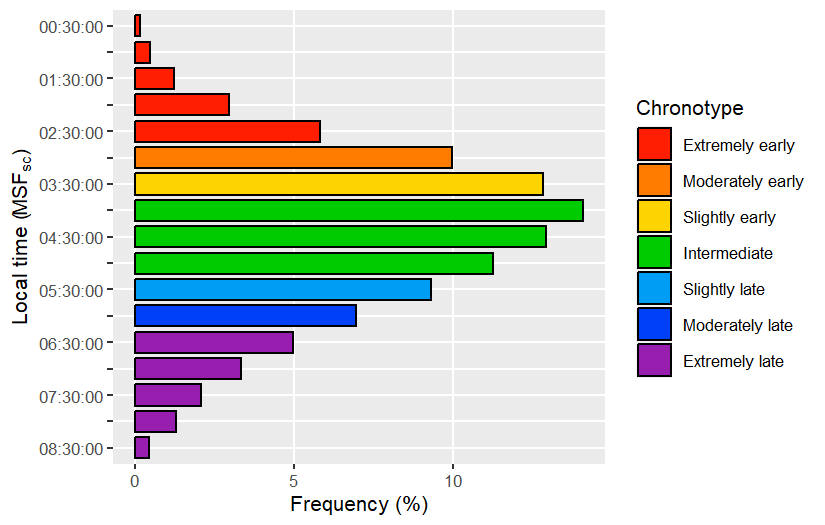
\includegraphics{qmd/chapter-6_files/figure-pdf/unnamed-chunk-4-1.png}

\legend{Source: Created by the author.}

}

\end{figure}%

The \(\text{MSF}_{\text{sc}}\) curve had a skewness of \(0.284\) and a
kurtosis of \(2.773\). However, the distribution was not normal
accordingly to Kolmogorov-Smirnov test (\(\text{D} = 0.03717\);
\(\text{p-value} = 2e-16\)) and D'Agostino Skewness test
(\(\text{Z3} = 31.525\); \(\text{p-value} = 2.2e-16\)).

A linear regression model was created with \(\text{MSF}_{\text{sc}}\) as
the response variable and with age and sex as predictors
(\(\text{R}^{2} = 0.05373\); \(\text{F}(2, 76741) = 2180\),
\(\text{p-value} = 2e-16\)), the two most known predictors for
chronotype (\textcite{roenneberg2007a}). A Box-Cox transformation of the
response variable was needed to attend to the linear regression model
assumptions (\(\lambda = -1.1111\);
\(\text{MSF}_{\text{sc}}^{\lambda - 1} / \lambda\)). All coefficients
were significantly different than \(0\) (\(\text{p-value} = 2e-16\))
and, accordingly to D'Agostino Skewness test, the residuals were normal
(\(\text{Z3} = -1.1906\); \(\text{p-value} = 0.23383\)). Residual
homoscedasticity was verified by a Score Test for Heteroskedasticity
(\(\chi^{2} = 0.00\); \(\text{p-value} = 1\)). No collinearity was found
between the predictor variables (variance inflation factor:
\(\text{age} = 1.0012\); \(\text{sex} = 1.0012\)).

Another model was created on top of the first one, adding the latitude
as a predictor variable (\(\text{R}^{2} = 0.060698\);
\(\text{F}(3, 76740) = 1650\), \(\text{p-value} = 2e-16\)). All
coefficients were significantly different than 0
(\(\text{p-value} = 2e-16\)) and the residuals were normally distributed
accordingly to the D'Agostino Skewness test, (\(\text{Z3} = 0.0742\);
\(\text{p-value} = 0.94085\)). Residual homoscedasticity was verified by
a Score Test for Heteroskedasticity (\(\chi^{2} = 0.00\);
\(\text{p-value} = 1\)). No collinearity was found between the predictor
variables (variance inflation factor: \(\text{age} = 1.0065\);
\(\text{sex} = 1.0016\); \$\text{latitude} = 1.0056 \$). The longitude
was not used as a predictor because it presented colinearity with the
latitude variable.

An \(\text{F}\) test for nested models showed a significant reduction of
the residual sum of squares (\(\text{F}(1, 76740) = 568.94\),
\(\text{p-value} = 2e-16\)), meaning that the latitude seems to produce
an effect on the chronotype. However, when estimating Cohen's \(f^2\)
effect size, the result was negligible \autocite{cohen1992}
\(((0.06069 - 0.05373) / (1 - 0.06069) = 0.00740\)).

\subsection{Discussion}\label{discussion}

The results show that even with a wide latitudinal spectrum and with a
big and aligned sample of biological states the latitude effect does not
reveal itself in a non-negligible size. Several studies indicate the
existence of this effect on the chronotype
\autocite{hut2013,leocadio-miguel2017,pittendrigh1991,randler2008,randler2017,roenneberg2003},
but, at this time, at least in humans, no empirical evidence can support
this claim. Our results are very similar to Leocadio-Miguel et al.
\autocite*{leocadio-miguel2017}, which also found a negligible effect
size (Cohen's \(f^{2} = 0.004143174\)). The inconsistency of the
latitude effect can be visualized in
Figure~\ref{fig-chapter-6-chronotype-distribution-by-latitude}.

\begin{Shaded}
\begin{Highlighting}[numbers=left,,]
\FunctionTok{source}\NormalTok{(here}\SpecialCharTok{::}\FunctionTok{here}\NormalTok{(}\StringTok{"R/plot\_latitude\_series.R"}\NormalTok{))}

\NormalTok{data }\SpecialCharTok{|\textgreater{}}
\NormalTok{  dplyr}\SpecialCharTok{::}\FunctionTok{filter}\NormalTok{(age }\SpecialCharTok{\textless{}=} \DecValTok{50}\NormalTok{) }\SpecialCharTok{|\textgreater{}}
  \FunctionTok{plot\_latitude\_series}\NormalTok{(}
    \AttributeTok{col =} \StringTok{"msf\_sc"}\NormalTok{, }
    \AttributeTok{y\_lab =}\NormalTok{ latex2exp}\SpecialCharTok{::}\FunctionTok{TeX}\NormalTok{(}\StringTok{"$MSF\_\{sc\} }\SpecialCharTok{\textbackslash{}\textbackslash{}}\StringTok{pm SEM$"}\NormalTok{), }
    \AttributeTok{line\_width =} \DecValTok{2}\NormalTok{, }
    \AttributeTok{point\_size =} \DecValTok{3}\NormalTok{,}
    \AttributeTok{error\_bar\_width =} \FloatTok{0.5}\NormalTok{, }
    \AttributeTok{error\_bar\_linewidth =} \DecValTok{1}\NormalTok{, }
    \AttributeTok{error\_bar =} \ConstantTok{TRUE}\NormalTok{,}
    \AttributeTok{text\_size =}\NormalTok{ env\_vars}\SpecialCharTok{$}\NormalTok{base\_size}
\NormalTok{  )}
\end{Highlighting}
\end{Shaded}

\begin{figure}[H]

\caption{\label{fig-chapter-6-chronotype-distribution-by-latitude}Distribution
of mean aggregates of the local time of the midpoint between sleep onset
and sleep end on work-free days (\(\text{MSF}_{\text{sc}}\)), MCTQ proxy
for measuring the chronotype, in relation to latitude decimal degree
intervals. Higher values of \(\text{MSF}_{\text{sc}}\) indicate a
tendency toward a late chronotype. The red line represents a linear
regression, and the shaded area indicates a pointwise 95\% confidence
interval.}

\centering{

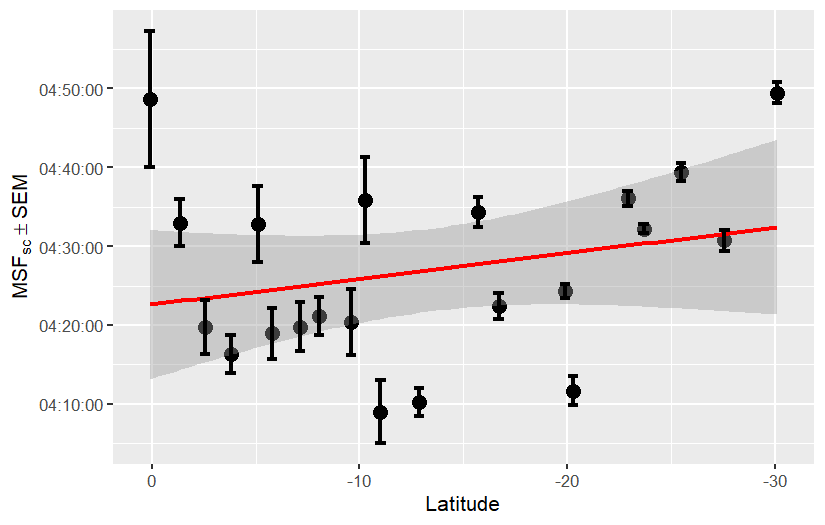
\includegraphics{qmd/chapter-6_files/figure-pdf/unnamed-chunk-5-1.png}

\legend{Source: Created by the author.}

}

\end{figure}%

Despite the lack of evidence, is not uncommon to hear talks insisting
that this effect is real and already proven. We suspect that this
behavior may be derived from a lack of understanding of statistical
models and techniques. Although it may be logical and aligned with the
overall theory for the evolution of biological temporal systems, it's
our role as scientists to eliminate contractions, not pursue them.

As Karl Popper said, science begins and ends with questions
\autocite{popper1979}. The absence of a strong entrainment with the
solar zeitgeber shows that the entrainment phenomenon is more complex
than we previously imagined. Other hypotheses for the human circadian
entrainment, like the entrainment to self-selected light, proposed by
Anna Skeldon and Derk-Jan Dijk \autocite*{skeldon2021}, need to be
tested and may produce significant results.

It's important to notice that the results shown here are preliminary.
The data still needs some cleaning and to be balanced with Brazil's
latest population census. The latitude coordinates used in the analysis
are related to the subject's state capital and, hence, have low
resolution. Even with these results, it may be that a significant
latitude effect can still appear at the end of the research.

Despite the several strengths that the dataset used in this study has,
it is also important to notice its weaknesses and limitations. The fact
that all the subjects were measured in the Spring season is one of them.
Since the objective is to catch individuals in different seasonal
patterns, the ideal moment to collect this kind of data is in the
wintertime, when there is a greater insolation gradient between the
equator and the poles. Another one is that this dataset can be
influenced by the presence of a Daylight Saving Time (DST) event. This
latter issue is explored in more detail in the methods section.

\section{Methods}\label{methods}

\subsection{Ethics information}\label{ethics-information}

Abiding by Brazilian law, all research involving human subjects must
have the approval of a Research Ethics Committee (REC) affiliated with
the
\href{https://conselho.saude.gov.br/Web_comissoes/conep/index.html}{Brazilian
National Research Ethics Committee (CONEP)}. This approval request is
ongoing (CAAE:
\href{https://plataformabrasil.saude.gov.br/login.jsf}{75588723.4.0000.5390}).

\subsection{Measurement instrument}\label{measurement-instrument}

Chronotypes were measured using the core version of the standard Munich
ChronoType Questionnaire (MCTQ) \autocite{roenneberg2003}. MCTQ is a
widely validated and widely used self-report questionnaire for measuring
the sleep-wake cycle and chronotypes \autocite{roenneberg2019}. It
quantifies the chronotype as a state, a biological circadian phenotype,
using as a proxy the local time of the midpoint between sleep onset and
sleep end on work-free days (\(MSF_{sc}\)). A sleep correction (SC) is
made when a possible sleep compensation related to a lack of sleep on
workdays is identified \autocite{roenneberg2012}.

Subjects were asked to complete an online questionnaire based on the
MCTQ Portuguese translation created by Till Roenneberg \& Martha Merrow
for the EUCLOCK project \autocite{roenneberg2006}
(\(\text{statements mean cosine distance} = 0.921\)). They were also
asked to provide sociodemographic (e.g., age, sex), geographic (e.g.,
full residential address), anthropometric (e.g., weight, height), and
work/study routine-related data. A deactivated version of the
questionnaire can be seen at \url{https://bit.ly/brchrono-form}.

\subsection{Sample}\label{sample}

The sample is made up of \(76,744\) Brazilian subjects. It was obtained
in 2017 from October 15th to 21st by a broadcast of the online research
questionnaire on a popular Sunday TV show with national reach
\autocite{globo2017}. This amount of data collected in such a short time
gave the sample a population cross-sectional characteristic.

A survey conducted in 2019 by the Brazilian Institute of Geography and
Statistics (IBGE) \autocite*{ibge2021} found that \(82.17\%\) of
Brazilian households had access to an internet connection. Therefore,
this sample is likely to have a good representation of Brazil's
population. Only residents of Brazilian states in the UTC-3 timezone,
aged \(18\) years or older, were included in the final sample.

In order to verify if the sample size was adequate for the study of the
phenomenon under investigation, a power analysis was conducted for
nested multiple regression models using the G*Power software
\autocite{faul2007}. The analysis used the parameters presented in
Leocadio-Miguel et al. \autocite*{leocadio-miguel2017} article for a
multiple linear regression with 10 tested predictors and only \(10\)
conceived predictors, considering a significance level of \(0.05\)
(\(\alpha\)) and a power of \(0.95\) (\(1 - \beta\)). The result showed
that a sample of \(5,895\) individuals would be necessary to test the
hypothesis.

Daylight Saving Time (DST) began in Brazil at midnight on November 15th,
2017. Residents from the Midwest, Southeast, and South regions were
instructed to set the clock forward by 1 hour. We believe that this
event did not contaminate the data since it started on the same day of
the data collection. It's important to notice that MCTQ asks subjects to
relate their routine behavior, not how they behaved in the last few
days. A possible effect of the DST on the sample is the production of an
even later chronotype for populations near the planet's poles,
amplifying a possible latitude effect. However, this was not shown on
the hypothesis test.

Based on the 2022 census \autocite{ibgea}, Brazil had \(52.263\%\) of
females and \(47.737\%\) of males with an age equal to or greater than
18 years old. The sample is skewed for female subjects, with
\(66.297\%\) of females and \(33.703\%\) of male subjects.

The subject's mean age is \(32.015\) years (\(\text{SD} = 9.252\);
\(\text{Max.} = 58.786\)). Female subjects have a mean age of \(31.787\)
years (\(\text{SD} = 9.364\); \(\text{Max.} = 58.786\)) and male
subjects \(32.464\) years (\(\text{SD} = 9.012\);
\(\text{Max.} = 58.772\)). For comparison, based on the 2022 census
\autocite{ibgeb}, Brazil's population with an age equal to or greater
than \(18\) years old had a mean age of \(44.277\) years
(\(\text{SD} = 17.221\)), with a mean age of \(44.987\) years
(\(\text{SD} = 17.511\)) for female subjects and a mean age of
\(43.499\) years (\(\text{SD} = 16.864\)) for male subjects.

Considering the five regions of Brazil, the sample is mostly skewed for
the Southeast, the most populated region. According to Brazil's 2022
census \autocite{ibge2022}, the Southeast region is home to \(41.784\%\)
of Brazil's population, followed by the Northeast (\(26.910\%\)), South
(\(14.741\%\)), North (\(8.544\%\)), and Midwest (\(8.021\%\)) regions.
\(62.454\%\) of the sample is located in the Southeast region,
\(11.797\%\) in the Northeast, \(17.861\%\) in the South, \(1.682\%\) in
the North, and \(6.205\%\) in the Midwest region. Note that a lack of
subjects in the North and Midwest region is justified by the sample
timezone inclusion criteria (UTC-3).

The sample latitudinal range was \(30.211\) decimal degrees
(\(\text{Min.} = -30.109\); \(\text{Max.} = 0.10177\)) with a
longitudinal span of \(16.378\) decimal degrees
(\(\text{Min.} = -51.342\); \(\text{Max.} = -34.964\)). For comparison,
Brazil has a latitudinal range of \(39.024\) decimal degrees
(\(\text{Min.} = -33.752\); \(\text{Max.} = 5.2719\)) and a longitudinal
span of \(39.198\) decimal degrees (\(\text{Min.} = -34.793\);
\(\text{Max.} = -73.991\)).

\textbf{The results shown in this article are just a preliminary view of
the data analysis}. The latitudes and longitudes of each subject are
represented by the coordinates of his/her state's capital (a low
resolution). The final results will have the latitude and longitude
coordinates based on the subject's postal codes and will also use a
balanced dataset following the latest Brazil census.

\subsection{Analysis}\label{analysis}

The data wrangling and analysis followed the data science program
proposed by Hadley Wickham and Garrett Grolemund \autocite{wickham2016}.
All processes were made with the help of the R programming language
\autocite{rcoreteam2023}, RStudio IDE \autocite{positteam2023}, and
several R packages. The tidyverse and rOpenSci package ecosystem and
other R packages adherents of the tidy tools manifesto
\autocite{wickham2023a} were prioritized. The MCTQ data was analyzed
using the \texttt{mctq} rOpenSci peer-reviewed package
\autocite{vartanian2023}. All processes were made in order to provide
result reproducibility and to be in accordance with the FAIR principles
\autocite{wilkinson2016}.

The study hypothesis was tested using nested models of multiple linear
regressions. The main idea of nested models is to verify the effect of
the inclusion of one or more predictors in the model variance
explanation (i.e., the \(\text{R}^{2}\)) \autocite{allen1997}. This can
be made by creating a restricted model and then comparing it with a full
model. Hence, the hypothesis can be schematized as follows.

\[
\begin{cases}
\text{H}_{0}: \text{R}^{2}_{\text{res}} >= \text{R}^{2}_{\text{full}} \\
\text{H}_{a}: \text{R}^{2}_{\text{res}} < \text{R}^{2}_{\text{full}}
\end{cases}
\]

\smallskip

In order to test a possible latitude association in predicting the
chronotype, the full model was the restricted model with the addition of
the latitude variable. The restricted model had the local time of the
midpoint between sleep onset and sleep end on work-free days
(\(\text{MSF}_{\text{sc}}\)) as the response variable, MCTQ proxy for
the chronotype, with sex and age as predictors.

A residual analysis was made to ensure the validity of the models before
the hypothesis test. The hypothesis was tested using a \(0.05\)
(\(\alpha\)) significance level.

To favor the alternative hypothesis (\(\text{H}_{a}\)), not only the
\(\text{R}^{2}\) of the full model must be significantly larger than the
\(\text{R}^{2}\) of the restricted model, but the effect size must be at
least considered small. To evaluate the effect size, Cohen's \(f^{2}\)
and his categorical parameters for size were used \autocite{cohen1992}.
That means that, in order to favor (\(\text{H}_{a}\)), the effect size
must be at least equal to or greater than \(0.0219\).

No blinding procedures were used during the analysis.

\subsection{Data availability}\label{data-availability}

The data that support the findings of this study are available from the
corresponding author {[}DV{]}. Restrictions apply to the availability of
these data, which were used under the approval of a Research Ethics
Committee (REC) linked to the
\href{https://conselho.saude.gov.br/Web_comissoes/conep/index.html}{Brazilian
National Research Ethics Committee (CONEP)}, hence it cannot be publicly
shared. Data are, however, available from the author upon reasonable
request and with CONEP approval.

\subsection{Code availability}\label{code-availability}

The research compendium of the project is available under the
\href{https://opensource.org/license/mit/}{MIT license} at
\url{https://github.com/danielvartan/mastersthesis}. The code has all
the steps from the raw data to the test results.

\section{Acknowledgments}\label{acknowledgments}

Financial support was provided by the
\href{https://www.gov.br/capes/}{Coordination for the Improvement of
Higher Education Personnel (CAPES)} and by the
\href{http://usp.br/}{University of Sao Paulo (USP)} (Grant number:
88887.703720/2022-00).

\section{Ethics declarations}\label{ethics-declarations}

\subsection{Competing interests}\label{competing-interests}

The author declares that the study was carried out without any
commercial or financial connections that could be seen as a possible
competing interest.

\section{Additional information}\label{additional-information}

\textbf{This manuscript shows only preliminary results and should not be
considered a document ready for journal submission.}

See the appendices section for supplementary information.

Correspondence can be sent to Daniel Vartanian
(\href{mailto:danvartan@gmail.com}{\nolinkurl{danvartan@gmail.com}}).

\section{Rights and permissions}\label{rights-and-permissions}

This article is released under the
\href{http://creativecommons.org/licenses/by/4.0/}{Creative Commons
Attribution 4.0 International License}, which permits use, sharing,
adaptation, distribution, and reproduction in any medium or format, as
long as be given appropriate credit to the original author and the
source, provide a link to the Creative Commons license, and indicate if
changes were made.

\bookmarksetup{startatroot}

\chapter{Discussion and conclusions}\label{discussion-and-conclusions}

\begin{tcolorbox}[enhanced jigsaw, colframe=quarto-callout-important-color-frame, coltitle=black, opacityback=0, left=2mm, opacitybacktitle=0.6, rightrule=.15mm, leftrule=.75mm, colbacktitle=quarto-callout-important-color!10!white, titlerule=0mm, title=\textcolor{quarto-callout-important-color}{\faExclamation}\hspace{0.5em}{Important}, colback=white, breakable, bottomtitle=1mm, toptitle=1mm, arc=.35mm, bottomrule=.15mm, toprule=.15mm]

You are reading the work-in-progress of this thesis.

\microskip

This chapter is currently a dumping ground for ideas, and I don't
recommend reading it.

\end{tcolorbox}

\postextual

\begingroup
\renewcommand{\baselinestretch}{1}
\setcounter{footnote}{0}
\renewcommand{\thefootnote}{\fnsymbol{footnote}}
\printbibliography[heading=bibheading]
\endgroup

\tocskipone
\tocprintchapternonum
\addcontentsline{toc}{chapter}{\newbibname}

\begin{glossario}

\bookmarksetup{startatroot}

\chapter*{Glossary}\label{glossary}
\addcontentsline{toc}{chapter}{Glossary}

\markboth{Glossary}{Glossary}

For an extensive list of chronobiology related terms and definitions,
please refer to \textcite{aschoff1965} and \textcite{marques2012}.

\begin{description}
\item[Chronotype]
\hspace{20cm}

Any kind of temporal phenotype \autocite{ehret1974,pittendrigh1993}.
Usually, it refers to circadian phenotypes in a spectrum that goes from
morningness to eveningness \autocite{roenneberg2003}. It can also be
seen as an organism's phase of entrainment \autocite{roenneberg2012a}.
\item[Circadian rhythm]
\hspace{20cm}

A rhythm with a period close to a day/24h, an approximation to the
period of the earth's rotation \autocite{pittendrigh1960}. From the
Latin \emph{circā}, around, and \emph{dĭes}, day \autocite{latinitium}.
Example: the sleep-wake cycle.
\item[Complex system]
\hspace{20cm}

There are several definitions. Here are some that I found to be of use:
\end{description}

\begin{itemize}
\tightlist
\item
  ``Systems that don't yield to compact forms of representation or
  description'' (David Krakauer apud \textcite{mitchell2013});
\item
  ``A system of many interacting parts where the system is more than
  just the sum of its parts'' (Mark Newman apud
  \textcite{mitchell2013});
\item
  Systems with many connected agents that interact and exhibit
  self-organization and emergence behavior, all without the need for a
  central controller (adapted from Camilo Rodrigues Neto's definition,
  supervisor of this thesis);
\item
  Dialectics at its finest (my working definition).
\end{itemize}

\begin{description}
\item[Entrainment]
\hspace{20cm}

A shift and alignment of biological rhythms induced by a zeitgeber input
\autocite{kuhlman2018}. For example: a shift/alignment of an organism's
circadian rhythm when exposed to light.
\end{description}

\begin{description}
\item[Infradian rhythm]
\hspace{20cm}

A rhythm with a period greater than a day/24h. From the Latin
\emph{infrā}, below (think in terms of period repetition), and
\emph{dĭes}, day \autocite{latinitium}. Example: the menstrual cycle.
\item[Period]
\hspace{20cm}

Cycle duration of an oscillation. In a more technical way, the duration
between two identical and consecutive phases in an oscillation
\autocite{kuhlman2018}.
\end{description}

\begin{description}
\item[System theory]
\hspace{20cm}

Two definitions can be of use:
\end{description}

\begin{itemize}
\tightlist
\item
  Science or discipline that investigates models, principles, and laws
  that are valid to systems in general \autocite{bertalanffy1968};
\item
  ``The attempt of a reductionist scientific tradition to come to terms
  with complexity, nonlinearity, and change through sophisticated
  mathematical and computational techniques, \emph{a groping toward a
  more dialectical understanding} that is held back by its philosophical
  biases and the institutional and economic contexts of its
  development'' \autocite{levins1998}.
\end{itemize}

\begin{description}
\item[Ultradian rhythm]
\hspace{20cm}

A rhythm with a period below a day/24h. From the Latin \emph{ultrā},
beyond (think in terms of period repetition), and \emph{dĭes}, day
\autocite{latinitium}. Example: the cardiac cycle.
\item[Zeitgeber]
\hspace{20cm}

Any periodic environmental signal/cue that can influence or regulate
biological rhythms. From the German \emph{zeit}, time, and \emph{geber},
donor \autocite{cambridgeuniversitypress}. Two main well known
zeitgebers are light exposure and environment temperature
\autocite{pittendrigh1960}.
\end{description}

\end{glossario}

\begin{apendicesenv}

\cleardoublepage
\phantomsection
\addcontentsline{toc}{part}{Appendices}
\appendix

\chapter{Chapter 2 supplemental
material}\label{chapter-2-supplemental-material}

\begin{tcolorbox}[enhanced jigsaw, colframe=quarto-callout-note-color-frame, coltitle=black, opacityback=0, left=2mm, opacitybacktitle=0.6, rightrule=.15mm, leftrule=.75mm, colbacktitle=quarto-callout-note-color!10!white, titlerule=0mm, title=\textcolor{quarto-callout-note-color}{\faInfo}\hspace{0.5em}{Note}, colback=white, breakable, bottomtitle=1mm, toptitle=1mm, arc=.35mm, bottomrule=.15mm, toprule=.15mm]

You are reading the work-in-progress of this thesis.

\microskip

This chapter should be readable but is currently undergoing final
polishing.

\end{tcolorbox}

\section{Base texts}\label{base-texts}

See \textcite{vartanian2017} to visualize the data questionnaire.

See \textcite{roenneberg2006} to visualize the EUCLOCK Portuguese
questionnaire.

See \textcite{reis2020} to learn more about the MCTQ\textsuperscript{PT}
questionnaire. It's important to note that the MCTQ\textsuperscript{PT}
was not included in the validation article. To obtain full access to the
questionnaire statements, you should contact the main author of the
article.

Two control texts were used, one from \textcite{andrade2023} and another
from \textcite{brecht2000}.

\begin{Shaded}
\begin{Highlighting}[numbers=left,,]
\NormalTok{data\_text }\OtherTok{\textless{}{-}} \FunctionTok{c}\NormalTok{(}
  \StringTok{"Você vai para a cama às \_\_\_ horas."}\NormalTok{,}
  \StringTok{"Algumas pessoas permanecem um tempo acordadas depois que vão se deitar."}\NormalTok{,}
  \StringTok{"Depois de ir para a cama, você decide dormir às \_\_\_ horas."}\NormalTok{,}
  \StringTok{"Você precisa de \_\_\_ para dormir."}\NormalTok{,}
  \StringTok{"Você acorda às \_\_\_ horas."}\NormalTok{,}
  \StringTok{"Você se levanta \_\_\_ depois de despertar."}\NormalTok{,}
  \StringTok{"Você vai para a cama às \_\_\_ horas."}\NormalTok{,}
  \StringTok{""}\NormalTok{,}
  \StringTok{"Depois de ir para a cama, você decide dormir às \_\_\_ horas."}\NormalTok{,}
  \StringTok{"Você precisa de \_\_\_ para dormir."}\NormalTok{,}
  \StringTok{"Você acorda às \_\_\_ horas."}\NormalTok{,}
  \StringTok{"Você se levanta \_\_\_ depois de despertar."}
\NormalTok{)}

\NormalTok{euclock\_text }\OtherTok{\textless{}{-}} \FunctionTok{c}\NormalTok{(}
  \StringTok{"vou para a cama às \_\_\_ horas."}\NormalTok{,}
  \StringTok{"Algumas pessoas permanecem um tempo acordadas depois que vão se deitar."}\NormalTok{,}
  \StringTok{"às \_\_\_ horas, decido dormir."}\NormalTok{,}
  \StringTok{"Eu necessito \_\_\_ minutos para adormecer."}\NormalTok{,}
  \StringTok{"acordo às \_\_\_ horas,"}\NormalTok{,}
  \StringTok{"passados \_\_\_ minutos, me levanto."}\NormalTok{,}
  \StringTok{"vou para a cama às \_\_\_ horas."}\NormalTok{,}
  \StringTok{"Algumas pessoas permanecem um tempo acordadas depois que vão se deitar."}\NormalTok{,}
  \StringTok{"às \_\_\_ horas, decido dormir."}\NormalTok{,}
  \StringTok{"Eu necessito \_\_\_ minutos para adormecer."}\NormalTok{,}
  \StringTok{"acordo às \_\_\_ horas,"}\NormalTok{,}
  \StringTok{"passados \_\_\_ minutos, me acordo."}
\NormalTok{)}

\NormalTok{mctq\_pt\_text }\OtherTok{\textless{}{-}} \FunctionTok{c}\NormalTok{(}
  \StringTok{"Vou para a cama às \_\_\_ horas."}\NormalTok{,}
  \StringTok{"Algumas pessoas permanecem algum tempo acordadas depois de estarem na cama."}\NormalTok{,}
  \StringTok{"Às \_\_\_ horas estou pronto para adormecer."}\NormalTok{,}
  \StringTok{"Necessito de \_\_\_ minutos para adormecer."}\NormalTok{,}
  \StringTok{"Acordo às \_\_\_ horas."}\NormalTok{,}
  \StringTok{"Após \_\_\_ minutos, levanto{-}me."}\NormalTok{,}
  \StringTok{"Vou para a cama às \_\_\_ horas."}\NormalTok{,}
  \StringTok{"Algumas pessoas permanecem algum tempo acordadas depois de estarem na cama."}\NormalTok{,}
  \StringTok{"Às \_\_\_ horas estou pronto para adormecer."}\NormalTok{,}
  \StringTok{"Necessito de \_\_\_ minutos para adormecer."}\NormalTok{,}
  \StringTok{"Acordo às \_\_\_ horas."}\NormalTok{,}
  \StringTok{"Após \_\_\_ minutos, levanto{-}me."}
\NormalTok{)}

\CommentTok{\# See: Andrade, T. (2023). Acronomia. In T. Andrade, Tau (Chapter 1). Flyve.}
\NormalTok{control\_text\_1 }\OtherTok{\textless{}{-}} \FunctionTok{c}\NormalTok{(}
  \StringTok{"Eles eliminaram o tempo, definitivamente."}\NormalTok{,}
  \StringTok{"Removeram todos os relógios, de parede, de pulso, de bolso..."}\NormalTok{,}
  \StringTok{"Talvez esses objetos fossem realmente obsoletos àquela altura"}\NormalTok{,}
  \StringTok{"mas sim, foi deliberado: era um projeto mundial."}\NormalTok{,}
  \StringTok{"Mas a situação é bem pior do que parece a princípio."}\NormalTok{,}
  \StringTok{"Não foi apenas qualquer possibilidade de aferição do tempo"}\NormalTok{,}
  \StringTok{"exterminaram a própria capacidade de produzi{-}lo."}\NormalTok{,}
  \StringTok{"Primeiro marcaram o \textquotesingle{}Grande dia da entrega\textquotesingle{}."}\NormalTok{,}
  \StringTok{"Um comboio de carros de lixo passou pelas ruas"}\NormalTok{,}
  \StringTok{"recolhendo todos os tipos de relógio"}\NormalTok{,}
  \StringTok{"e cronômetro que estavam de posse das pessoas."}\NormalTok{,}
  \StringTok{"De mecanismos empoeirados e engrenagens enferrujadas a dispositivos modernos"}
\NormalTok{)}

\CommentTok{\# See: Brecht, B. (2000). Quem se defende. In B. Brecht, Poemas 1913{-}1956 }
\CommentTok{\#      (5th ed., p. 73; Paulo César de Souza, Trans.). Editora 34.}
\NormalTok{control\_text\_2 }\OtherTok{\textless{}{-}} \FunctionTok{c}\NormalTok{(}
  \StringTok{"Quem se defende porque lhe tiram o ar"}\NormalTok{,}
  \StringTok{"Ao lhe apertar a garganta, "}\NormalTok{,}
  \StringTok{"para este há um parágrafo"}\NormalTok{,}
  \StringTok{"Que diz: ele agiu em legítima defesa. "}\NormalTok{, }
  \StringTok{"Mas"}\NormalTok{,}
  \StringTok{"O mesmo parágrafo silencia"}\NormalTok{,}
  \StringTok{"Quando vocês se defendem porque lhes tiram o pão."}\NormalTok{,}
  \StringTok{"E no entanto morre quem não come, "}\NormalTok{,}
  \StringTok{"e quem não come o suficiente"}\NormalTok{,}
  \StringTok{"Morre lentamente. "}\NormalTok{,}
  \StringTok{"Durante os anos todos em que morre"}\NormalTok{,}
  \StringTok{"Não lhe é permitido se defender."}
\NormalTok{)}
\end{Highlighting}
\end{Shaded}

\begin{Shaded}
\begin{Highlighting}[numbers=left,,]
\NormalTok{data\_text\_textreuse }\OtherTok{\textless{}{-}} 
\NormalTok{  textreuse}\SpecialCharTok{::}\FunctionTok{TextReuseTextDocument}\NormalTok{(}
    \AttributeTok{text =}\NormalTok{ data\_text,}
    \AttributeTok{meta =} \FunctionTok{list}\NormalTok{(}\AttributeTok{id =} \StringTok{"data"}\NormalTok{)}
\NormalTok{  )}

\NormalTok{euclock\_text\_textreuse }\OtherTok{\textless{}{-}} 
\NormalTok{  textreuse}\SpecialCharTok{::}\FunctionTok{TextReuseTextDocument}\NormalTok{(}
    \AttributeTok{text =}\NormalTok{ euclock\_text,}
    \AttributeTok{meta =} \FunctionTok{list}\NormalTok{(}\AttributeTok{id =} \StringTok{"euclock"}\NormalTok{)}
\NormalTok{  )}

\NormalTok{mctq\_pt\_text\_textreuse }\OtherTok{\textless{}{-}} 
\NormalTok{  textreuse}\SpecialCharTok{::}\FunctionTok{TextReuseTextDocument}\NormalTok{(}
    \AttributeTok{text =}\NormalTok{ mctq\_pt\_text,}
    \AttributeTok{meta =} \FunctionTok{list}\NormalTok{(}\AttributeTok{id =} \StringTok{"mctq\_pt"}\NormalTok{)}
\NormalTok{  )}

\NormalTok{control\_text\_1\_textreuse }\OtherTok{\textless{}{-}} 
\NormalTok{  textreuse}\SpecialCharTok{::}\FunctionTok{TextReuseTextDocument}\NormalTok{(}
    \AttributeTok{text =}\NormalTok{ control\_text\_1,}
    \AttributeTok{meta =} \FunctionTok{list}\NormalTok{(}\AttributeTok{id =} \StringTok{"control\_1"}\NormalTok{)}
\NormalTok{  )}

\NormalTok{control\_text\_2\_textreuse }\OtherTok{\textless{}{-}} 
\NormalTok{  textreuse}\SpecialCharTok{::}\FunctionTok{TextReuseTextDocument}\NormalTok{(}
    \AttributeTok{text =}\NormalTok{ control\_text\_2,}
    \AttributeTok{meta =} \FunctionTok{list}\NormalTok{(}\AttributeTok{id =} \StringTok{"control\_2"}\NormalTok{)}
\NormalTok{  )}
\end{Highlighting}
\end{Shaded}

\begin{Shaded}
\begin{Highlighting}[numbers=left,,]
\CommentTok{\# See}
\CommentTok{\# \textless{}https://huggingface.co/neuralmind/bert{-}base{-}portuguese{-}cased\textgreater{}}
\CommentTok{\# to learn more.}

\NormalTok{rutils}\SpecialCharTok{:::}\FunctionTok{assert\_internet}\NormalTok{()}

\NormalTok{text\_embed }\OtherTok{\textless{}{-}} \ControlFlowTok{function}\NormalTok{(text) \{}
\NormalTok{  checkmate}\SpecialCharTok{::}\FunctionTok{assert\_character}\NormalTok{(text)}
  
\NormalTok{  text }\SpecialCharTok{|\textgreater{}}
\NormalTok{    text}\SpecialCharTok{::}\FunctionTok{textEmbed}\NormalTok{(}
      \AttributeTok{model =} \StringTok{"neuralmind/bert{-}base{-}portuguese{-}cased"}\NormalTok{,}
      \AttributeTok{layers =} \SpecialCharTok{{-}} \DecValTok{2}\NormalTok{,}
      \AttributeTok{dim\_name =} \ConstantTok{TRUE}\NormalTok{,}
      \AttributeTok{aggregation\_from\_layers\_to\_tokens =} \StringTok{"concatenate"}\NormalTok{,}
      \AttributeTok{aggregation\_from\_tokens\_to\_texts =} \StringTok{"mean"}\NormalTok{,}
      \AttributeTok{aggregation\_from\_tokens\_to\_word\_types =} \ConstantTok{NULL}\NormalTok{,}
      \AttributeTok{keep\_token\_embeddings =} \ConstantTok{TRUE}\NormalTok{,}
      \AttributeTok{tokens\_select =} \ConstantTok{NULL}\NormalTok{,}
      \AttributeTok{tokens\_deselect =} \ConstantTok{NULL}\NormalTok{,}
      \AttributeTok{decontextualize =} \ConstantTok{FALSE}\NormalTok{,}
      \AttributeTok{model\_max\_length =} \ConstantTok{NULL}\NormalTok{,}
      \AttributeTok{max\_token\_to\_sentence =} \DecValTok{4}\NormalTok{,}
      \AttributeTok{tokenizer\_parallelism =} \ConstantTok{FALSE}\NormalTok{,}
      \AttributeTok{device =} \StringTok{"gpu"}\NormalTok{,}
      \AttributeTok{logging\_level =} \StringTok{"error"}
\NormalTok{    )}
\NormalTok{\}}

\NormalTok{data\_text\_textembed }\OtherTok{\textless{}{-}} \FunctionTok{text\_embed}\NormalTok{(data\_text)}
\NormalTok{euclock\_text\_textembed }\OtherTok{\textless{}{-}} \FunctionTok{text\_embed}\NormalTok{(euclock\_text)}
\NormalTok{mctq\_pt\_text\_textembed }\OtherTok{\textless{}{-}} \FunctionTok{text\_embed}\NormalTok{(mctq\_pt\_text)}
\NormalTok{control\_text\_1\_textembed }\OtherTok{\textless{}{-}} \FunctionTok{text\_embed}\NormalTok{(control\_text\_1)}
\NormalTok{control\_text\_2\_textembed }\OtherTok{\textless{}{-}} \FunctionTok{text\_embed}\NormalTok{(control\_text\_2)}
\end{Highlighting}
\end{Shaded}

\section{Text similarity}\label{text-similarity}

See \textcite{wang2020} to learn more.

For a quick explanation, see \url{https://youtu.be/e9U0QAFbfLI}.

\begin{Shaded}
\begin{Highlighting}[numbers=left,,]
\NormalTok{text\_distance }\OtherTok{\textless{}{-}} \ControlFlowTok{function}\NormalTok{(x, y) \{}
\NormalTok{  checkmate}\SpecialCharTok{::}\FunctionTok{assert\_list}\NormalTok{(x, }\AttributeTok{len =} \DecValTok{2}\NormalTok{)}
\NormalTok{  checkmate}\SpecialCharTok{::}\FunctionTok{assert\_list}\NormalTok{(y, }\AttributeTok{len =} \DecValTok{2}\NormalTok{)}
  
\NormalTok{  methods }\OtherTok{\textless{}{-}} \FunctionTok{c}\NormalTok{(}
    \StringTok{"binary"}\NormalTok{, }\StringTok{"cosine"}\NormalTok{, }\StringTok{"canberra"}\NormalTok{, }\StringTok{"euclidean"}\NormalTok{, }\StringTok{"manhattan"}\NormalTok{, }\StringTok{"maximum"}\NormalTok{, }
    \StringTok{"minkowski"}\NormalTok{, }\StringTok{"pearson"}
\NormalTok{  )}
  
  \ControlFlowTok{for}\NormalTok{ (i }\ControlFlowTok{in}\NormalTok{ methods) \{}
\NormalTok{    cli}\SpecialCharTok{::}\FunctionTok{cli\_alert\_info}\NormalTok{(}\FunctionTok{paste0}\NormalTok{(}
      \StringTok{"Method: \{.strong \{stringr::str\_to\_title(i)\}\}"}
\NormalTok{      ))}
    
\NormalTok{    test }\OtherTok{\textless{}{-}} 
\NormalTok{      text}\SpecialCharTok{::}\FunctionTok{textSimilarity}\NormalTok{(}
\NormalTok{        x}\SpecialCharTok{$}\NormalTok{texts}\SpecialCharTok{$}\NormalTok{texts, }
\NormalTok{        y}\SpecialCharTok{$}\NormalTok{texts}\SpecialCharTok{$}\NormalTok{texts, }
        \AttributeTok{method =}\NormalTok{ i, }
        \AttributeTok{center =} \ConstantTok{TRUE}\NormalTok{, }
        \AttributeTok{scale =} \ConstantTok{FALSE}
\NormalTok{      )}
    
\NormalTok{    cli}\SpecialCharTok{::}\FunctionTok{cli\_bullets}\NormalTok{(}\FunctionTok{c}\NormalTok{(}\StringTok{"\textgreater{}"} \OtherTok{=} \StringTok{"Line by line"}\NormalTok{))}
    \FunctionTok{print}\NormalTok{(test)}
    
\NormalTok{    cli}\SpecialCharTok{::}\FunctionTok{cli\_bullets}\NormalTok{(}\FunctionTok{c}\NormalTok{(}\StringTok{"\textgreater{}"} \OtherTok{=} \StringTok{"Overall mean"}\NormalTok{))}
    \FunctionTok{print}\NormalTok{(}\FunctionTok{mean}\NormalTok{(test))}
    
\NormalTok{    cli}\SpecialCharTok{::}\FunctionTok{cat\_line}\NormalTok{()}
\NormalTok{  \}}
\NormalTok{\}}
\end{Highlighting}
\end{Shaded}

\begin{Shaded}
\begin{Highlighting}[numbers=left,,]
\NormalTok{text\_representation }\OtherTok{\textless{}{-}} \ControlFlowTok{function}\NormalTok{(x, y) \{}
\NormalTok{  checkmate}\SpecialCharTok{::}\FunctionTok{assert\_class}\NormalTok{(x, }\StringTok{"TextReuseTextDocument"}\NormalTok{)}
\NormalTok{  checkmate}\SpecialCharTok{::}\FunctionTok{assert\_class}\NormalTok{(y, }\StringTok{"TextReuseTextDocument"}\NormalTok{)}
  
\NormalTok{  cli}\SpecialCharTok{::}\FunctionTok{cli\_alert\_info}\NormalTok{(}\FunctionTok{paste0}\NormalTok{(}\StringTok{"Method: \{.strong Jaccard similarity\}"}\NormalTok{))}
  \FunctionTok{print}\NormalTok{(textreuse}\SpecialCharTok{::}\FunctionTok{jaccard\_similarity}\NormalTok{(x, y))}
\NormalTok{  cli}\SpecialCharTok{::}\FunctionTok{cat\_line}\NormalTok{()}
  
\NormalTok{  cli}\SpecialCharTok{::}\FunctionTok{cli\_alert\_info}\NormalTok{(}\FunctionTok{paste0}\NormalTok{(}\StringTok{"Method: \{.strong Jaccard bag similarity\}"}\NormalTok{))}
  \FunctionTok{print}\NormalTok{(textreuse}\SpecialCharTok{::}\FunctionTok{jaccard\_bag\_similarity}\NormalTok{(x, y))}
\NormalTok{  cli}\SpecialCharTok{::}\FunctionTok{cat\_line}\NormalTok{()}
\NormalTok{\}}
\end{Highlighting}
\end{Shaded}

\subsection{\texorpdfstring{How similar is the \emph{data questionnaire}
when compared to the \emph{EUCLOCK
questionnaire}?}{How similar is the data questionnaire when compared to the EUCLOCK questionnaire?}}\label{how-similar-is-the-data-questionnaire-when-compared-to-the-euclock-questionnaire}

\subsubsection{Text distance}\label{text-distance}

\begin{Shaded}
\begin{Highlighting}[numbers=left,,]
\FunctionTok{text\_distance}\NormalTok{(data\_text\_textembed, euclock\_text\_textembed)}
\CommentTok{\#\textgreater{} i Method: Binary}
\CommentTok{\#\textgreater{} \textgreater{} Line by line}
\CommentTok{\#\textgreater{}  [1] 1 1 1 1 1 1 1 1 1 1 1 1}
\CommentTok{\#\textgreater{} \textgreater{} Overall mean}
\CommentTok{\#\textgreater{} [1] 1}
\CommentTok{\#\textgreater{} i Method: Cosine}
\CommentTok{\#\textgreater{} \textgreater{} Line by line}
\CommentTok{\#\textgreater{}  [1] 0.9911730 1.0000000 0.9639984 0.9662432 0.9604119 0.9557896 0.9911730}
\CommentTok{\#\textgreater{}  [8] 0.1559853 0.9639984 0.9662432 0.9604119 0.9497428}
\CommentTok{\#\textgreater{} \textgreater{} Overall mean}
\CommentTok{\#\textgreater{} [1] 0.9020976}
\CommentTok{\#\textgreater{} i Method: Canberra}
\CommentTok{\#\textgreater{} \textgreater{} Line by line}
\CommentTok{\#\textgreater{}  [1] {-}218.3367    1.0000 {-}335.1895 {-}318.9419 {-}335.9000 {-}373.7989 {-}218.3367}
\CommentTok{\#\textgreater{}  [8] {-}642.5522 {-}335.1895 {-}318.9419 {-}335.9000 {-}381.4067}
\CommentTok{\#\textgreater{} \textgreater{} Overall mean}
\CommentTok{\#\textgreater{} [1] {-}317.7912}
\CommentTok{\#\textgreater{} i Method: Euclidean}
\CommentTok{\#\textgreater{} \textgreater{} Line by line}
\CommentTok{\#\textgreater{}  [1]  {-}1.504474   1.000000  {-}4.058168  {-}3.976768  {-}4.144779  {-}4.705653}
\CommentTok{\#\textgreater{}  [7]  {-}1.504474 {-}19.453535  {-}4.058168  {-}3.976768  {-}4.144779  {-}5.071087}
\CommentTok{\#\textgreater{} \textgreater{} Overall mean}
\CommentTok{\#\textgreater{} [1] {-}4.633221}
\CommentTok{\#\textgreater{} i Method: Manhattan}
\CommentTok{\#\textgreater{} \textgreater{} Line by line}
\CommentTok{\#\textgreater{}  [1]  {-}53.58509    1.00000 {-}108.96057 {-}105.53439 {-}111.46668 {-}124.16400}
\CommentTok{\#\textgreater{}  [7]  {-}53.58509 {-}198.94244 {-}108.96057 {-}105.53439 {-}111.46668 {-}131.16054}
\CommentTok{\#\textgreater{} \textgreater{} Overall mean}
\CommentTok{\#\textgreater{} [1] {-}101.03}
\CommentTok{\#\textgreater{} i Method: Maximum}
\CommentTok{\#\textgreater{} \textgreater{} Line by line}
\CommentTok{\#\textgreater{}  [1]   0.52944993   1.00000000   0.37664773   0.07405534   0.11978415}
\CommentTok{\#\textgreater{}  [6]   0.31058226   0.52944993 {-}14.91353795   0.37664773   0.07405534}
\CommentTok{\#\textgreater{} [11]   0.11978415   0.16830817}
\CommentTok{\#\textgreater{} \textgreater{} Overall mean}
\CommentTok{\#\textgreater{} [1] {-}0.9362311}
\CommentTok{\#\textgreater{} i Method: Minkowski}
\CommentTok{\#\textgreater{} \textgreater{} Line by line}
\CommentTok{\#\textgreater{}  [1]  {-}1.504474   1.000000  {-}4.058168  {-}3.976768  {-}4.144779  {-}4.705653}
\CommentTok{\#\textgreater{}  [7]  {-}1.504474 {-}19.453535  {-}4.058168  {-}3.976768  {-}4.144779  {-}5.071087}
\CommentTok{\#\textgreater{} \textgreater{} Overall mean}
\CommentTok{\#\textgreater{} [1] {-}4.633221}
\CommentTok{\#\textgreater{} i Method: Pearson}
\CommentTok{\#\textgreater{} \textgreater{} Line by line}
\CommentTok{\#\textgreater{}  [1] 0.9911730 1.0000000 0.9639984 0.9662432 0.9604119 0.9557896 0.9911730}
\CommentTok{\#\textgreater{}  [8] 0.1559853 0.9639984 0.9662432 0.9604119 0.9497428}
\CommentTok{\#\textgreater{} \textgreater{} Overall mean}
\CommentTok{\#\textgreater{} [1] 0.9020976}
\end{Highlighting}
\end{Shaded}

\subsubsection{Text representation}\label{text-representation}

\textbf{Note}: The maximum value for the Jaccard bag similarity is 0.5.

\begin{Shaded}
\begin{Highlighting}[numbers=left,,]
\FunctionTok{text\_representation}\NormalTok{(euclock\_text\_textreuse, data\_text\_textreuse)}
\CommentTok{\#\textgreater{} i Method: Jaccard similarity}
\CommentTok{\#\textgreater{} [1] 0.2173913}
\CommentTok{\#\textgreater{} i Method: Jaccard bag similarity}
\CommentTok{\#\textgreater{} [1] 0.1446541}
\end{Highlighting}
\end{Shaded}

\subsection{\texorpdfstring{How similar is the \emph{data questionnaire}
when compared to the \emph{MCTQ\textsuperscript{PT}
questionnaire}?}{How similar is the data questionnaire when compared to the MCTQPT questionnaire?}}\label{how-similar-is-the-data-questionnaire-when-compared-to-the-mctqpt-questionnaire}

\subsubsection{Text distance}\label{text-distance-1}

\begin{Shaded}
\begin{Highlighting}[numbers=left,,]
\FunctionTok{text\_distance}\NormalTok{(data\_text\_textembed, mctq\_pt\_text\_textembed)}
\CommentTok{\#\textgreater{} i Method: Binary}
\CommentTok{\#\textgreater{} \textgreater{} Line by line}
\CommentTok{\#\textgreater{}  [1] 1 1 1 1 1 1 1 1 1 1 1 1}
\CommentTok{\#\textgreater{} \textgreater{} Overall mean}
\CommentTok{\#\textgreater{} [1] 1}
\CommentTok{\#\textgreater{} i Method: Cosine}
\CommentTok{\#\textgreater{} \textgreater{} Line by line}
\CommentTok{\#\textgreater{}  [1] 0.9901437 0.9898982 0.9687513 0.9575260 0.9882873 0.9598702 0.9901437}
\CommentTok{\#\textgreater{}  [8] 0.1601500 0.9687513 0.9575260 0.9882873 0.9598702}
\CommentTok{\#\textgreater{} \textgreater{} Overall mean}
\CommentTok{\#\textgreater{} [1] 0.9066005}
\CommentTok{\#\textgreater{} i Method: Canberra}
\CommentTok{\#\textgreater{} \textgreater{} Line by line}
\CommentTok{\#\textgreater{}  [1] {-}227.9938 {-}247.6044 {-}335.9297 {-}349.9493 {-}225.4809 {-}353.5263 {-}227.9938}
\CommentTok{\#\textgreater{}  [8] {-}631.6228 {-}335.9297 {-}349.9493 {-}225.4809 {-}353.5263}
\CommentTok{\#\textgreater{} \textgreater{} Overall mean}
\CommentTok{\#\textgreater{} [1] {-}322.0823}
\CommentTok{\#\textgreater{} i Method: Euclidean}
\CommentTok{\#\textgreater{} \textgreater{} Line by line}
\CommentTok{\#\textgreater{}  [1]  {-}1.662187  {-}1.729814  {-}3.807963  {-}4.603019  {-}1.810249  {-}4.458696}
\CommentTok{\#\textgreater{}  [7]  {-}1.662187 {-}19.380367  {-}3.807963  {-}4.603019  {-}1.810249  {-}4.458696}
\CommentTok{\#\textgreater{} \textgreater{} Overall mean}
\CommentTok{\#\textgreater{} [1] {-}4.482867}
\CommentTok{\#\textgreater{} i Method: Manhattan}
\CommentTok{\#\textgreater{} \textgreater{} Line by line}
\CommentTok{\#\textgreater{}  [1]  {-}57.28537  {-}58.97985 {-}102.26048 {-}119.55311  {-}59.76706 {-}117.55850}
\CommentTok{\#\textgreater{}  [7]  {-}57.28537 {-}193.79964 {-}102.26048 {-}119.55311  {-}59.76706 {-}117.55850}
\CommentTok{\#\textgreater{} \textgreater{} Overall mean}
\CommentTok{\#\textgreater{} [1] {-}97.13571}
\CommentTok{\#\textgreater{} i Method: Maximum}
\CommentTok{\#\textgreater{} \textgreater{} Line by line}
\CommentTok{\#\textgreater{}  [1]   0.60554241   0.60396075   0.41795957   0.01856209   0.39220500}
\CommentTok{\#\textgreater{}  [6]   0.28932291   0.60554241 {-}14.95654231   0.41795957   0.01856209}
\CommentTok{\#\textgreater{} [11]   0.39220500   0.28932291}
\CommentTok{\#\textgreater{} \textgreater{} Overall mean}
\CommentTok{\#\textgreater{} [1] {-}0.9087831}
\CommentTok{\#\textgreater{} i Method: Minkowski}
\CommentTok{\#\textgreater{} \textgreater{} Line by line}
\CommentTok{\#\textgreater{}  [1]  {-}1.662187  {-}1.729814  {-}3.807963  {-}4.603019  {-}1.810249  {-}4.458696}
\CommentTok{\#\textgreater{}  [7]  {-}1.662187 {-}19.380367  {-}3.807963  {-}4.603019  {-}1.810249  {-}4.458696}
\CommentTok{\#\textgreater{} \textgreater{} Overall mean}
\CommentTok{\#\textgreater{} [1] {-}4.482867}
\CommentTok{\#\textgreater{} i Method: Pearson}
\CommentTok{\#\textgreater{} \textgreater{} Line by line}
\CommentTok{\#\textgreater{}  [1] 0.9901437 0.9898982 0.9687513 0.9575260 0.9882873 0.9598702 0.9901437}
\CommentTok{\#\textgreater{}  [8] 0.1601500 0.9687513 0.9575260 0.9882873 0.9598702}
\CommentTok{\#\textgreater{} \textgreater{} Overall mean}
\CommentTok{\#\textgreater{} [1] 0.9066005}
\end{Highlighting}
\end{Shaded}

\subsubsection{Text representation}\label{text-representation-1}

\textbf{Note}: The maximum value for the Jaccard bag similarity is 0.5.

\begin{Shaded}
\begin{Highlighting}[numbers=left,,]
\FunctionTok{text\_representation}\NormalTok{(mctq\_pt\_text\_textreuse, data\_text\_textreuse)}
\CommentTok{\#\textgreater{} i Method: Jaccard similarity}
\CommentTok{\#\textgreater{} [1] 0.1052632}
\CommentTok{\#\textgreater{} i Method: Jaccard bag similarity}
\CommentTok{\#\textgreater{} [1] 0.09815951}
\end{Highlighting}
\end{Shaded}

\subsection{\texorpdfstring{How similar is the \emph{data questionnaire}
when compared to the \emph{Control Text
1}?}{How similar is the data questionnaire when compared to the Control Text 1?}}\label{how-similar-is-the-data-questionnaire-when-compared-to-the-control-text-1}

\subsubsection{Text distance}\label{text-distance-2}

\begin{Shaded}
\begin{Highlighting}[numbers=left,,]
\FunctionTok{text\_distance}\NormalTok{(data\_text\_textembed, control\_text\_1\_textembed)}
\CommentTok{\#\textgreater{} i Method: Binary}
\CommentTok{\#\textgreater{} \textgreater{} Line by line}
\CommentTok{\#\textgreater{}  [1] 1 1 1 1 1 1 1 1 1 1 1 1}
\CommentTok{\#\textgreater{} \textgreater{} Overall mean}
\CommentTok{\#\textgreater{} [1] 1}
\CommentTok{\#\textgreater{} i Method: Cosine}
\CommentTok{\#\textgreater{} \textgreater{} Line by line}
\CommentTok{\#\textgreater{}  [1] 0.9050224 0.8904954 0.8996243 0.8864538 0.8587490 0.8921112 0.8880434}
\CommentTok{\#\textgreater{}  [8] 0.1887362 0.8882691 0.8727013 0.8732868 0.8433085}
\CommentTok{\#\textgreater{} \textgreater{} Overall mean}
\CommentTok{\#\textgreater{} [1] 0.8239001}
\CommentTok{\#\textgreater{} i Method: Canberra}
\CommentTok{\#\textgreater{} \textgreater{} Line by line}
\CommentTok{\#\textgreater{}  [1] {-}469.3314 {-}485.1504 {-}483.8301 {-}506.1996 {-}504.6484 {-}490.3147 {-}478.4438}
\CommentTok{\#\textgreater{}  [8] {-}632.5119 {-}492.0333 {-}490.9512 {-}496.6430 {-}517.2764}
\CommentTok{\#\textgreater{} \textgreater{} Overall mean}
\CommentTok{\#\textgreater{} [1] {-}503.9445}
\CommentTok{\#\textgreater{} i Method: Euclidean}
\CommentTok{\#\textgreater{} \textgreater{} Line by line}
\CommentTok{\#\textgreater{}  [1]  {-}7.299638  {-}7.859283  {-}7.547236  {-}8.207869  {-}8.889088  {-}8.131165}
\CommentTok{\#\textgreater{}  [7]  {-}8.090413 {-}18.891223  {-}7.834767  {-}8.892308  {-}8.472040  {-}9.696238}
\CommentTok{\#\textgreater{} \textgreater{} Overall mean}
\CommentTok{\#\textgreater{} [1] {-}9.150939}
\CommentTok{\#\textgreater{} i Method: Manhattan}
\CommentTok{\#\textgreater{} \textgreater{} Line by line}
\CommentTok{\#\textgreater{}  [1] {-}174.9785 {-}191.0842 {-}182.5955 {-}197.5195 {-}212.8954 {-}196.0854 {-}196.2141}
\CommentTok{\#\textgreater{}  [8] {-}181.0755 {-}192.3436 {-}212.1597 {-}198.4904 {-}233.2716}
\CommentTok{\#\textgreater{} \textgreater{} Overall mean}
\CommentTok{\#\textgreater{} [1] {-}197.3928}
\CommentTok{\#\textgreater{} i Method: Maximum}
\CommentTok{\#\textgreater{} \textgreater{} Line by line}
\CommentTok{\#\textgreater{}  [1]  {-}0.1064962  {-}0.1808311  {-}0.2100441  {-}0.3340142  {-}0.3991810  {-}0.4304202}
\CommentTok{\#\textgreater{}  [7]  {-}0.1888392 {-}15.1616240  {-}0.4010140  {-}0.9773587  {-}0.4897276  {-}0.6558742}
\CommentTok{\#\textgreater{} \textgreater{} Overall mean}
\CommentTok{\#\textgreater{} [1] {-}1.627952}
\CommentTok{\#\textgreater{} i Method: Minkowski}
\CommentTok{\#\textgreater{} \textgreater{} Line by line}
\CommentTok{\#\textgreater{}  [1]  {-}7.299638  {-}7.859283  {-}7.547236  {-}8.207869  {-}8.889088  {-}8.131165}
\CommentTok{\#\textgreater{}  [7]  {-}8.090413 {-}18.891223  {-}7.834767  {-}8.892308  {-}8.472040  {-}9.696238}
\CommentTok{\#\textgreater{} \textgreater{} Overall mean}
\CommentTok{\#\textgreater{} [1] {-}9.150939}
\CommentTok{\#\textgreater{} i Method: Pearson}
\CommentTok{\#\textgreater{} \textgreater{} Line by line}
\CommentTok{\#\textgreater{}  [1] 0.9050224 0.8904954 0.8996243 0.8864538 0.8587490 0.8921112 0.8880434}
\CommentTok{\#\textgreater{}  [8] 0.1887362 0.8882691 0.8727013 0.8732868 0.8433085}
\CommentTok{\#\textgreater{} \textgreater{} Overall mean}
\CommentTok{\#\textgreater{} [1] 0.8239001}
\end{Highlighting}
\end{Shaded}

\subsubsection{Text representation}\label{text-representation-2}

\begin{Shaded}
\begin{Highlighting}[numbers=left,,]
\FunctionTok{text\_representation}\NormalTok{(control\_text\_1\_textreuse, data\_text\_textreuse)}
\CommentTok{\#\textgreater{} i Method: Jaccard similarity}
\CommentTok{\#\textgreater{} [1] 0}
\CommentTok{\#\textgreater{} i Method: Jaccard bag similarity}
\CommentTok{\#\textgreater{} [1] 0}
\end{Highlighting}
\end{Shaded}

\subsection{\texorpdfstring{How similar is the \emph{data questionnaire}
when compared to the \emph{Control Text
2}?}{How similar is the data questionnaire when compared to the Control Text 2?}}\label{how-similar-is-the-data-questionnaire-when-compared-to-the-control-text-2}

\subsubsection{Text distance}\label{text-distance-3}

\begin{Shaded}
\begin{Highlighting}[numbers=left,,]
\FunctionTok{text\_distance}\NormalTok{(data\_text\_textembed, control\_text\_2\_textembed)}
\CommentTok{\#\textgreater{} i Method: Binary}
\CommentTok{\#\textgreater{} \textgreater{} Line by line}
\CommentTok{\#\textgreater{}  [1] 1 1 1 1 1 1 1 1 1 1 1 1}
\CommentTok{\#\textgreater{} \textgreater{} Overall mean}
\CommentTok{\#\textgreater{} [1] 1}
\CommentTok{\#\textgreater{} i Method: Cosine}
\CommentTok{\#\textgreater{} \textgreater{} Line by line}
\CommentTok{\#\textgreater{}  [1] 0.9060095 0.9037570 0.8737437 0.8856842 0.7641104 0.9035066 0.9119419}
\CommentTok{\#\textgreater{}  [8] 0.2057337 0.8851267 0.9036579 0.8678450 0.9198303}
\CommentTok{\#\textgreater{} \textgreater{} Overall mean}
\CommentTok{\#\textgreater{} [1] 0.8275789}
\CommentTok{\#\textgreater{} i Method: Canberra}
\CommentTok{\#\textgreater{} \textgreater{} Line by line}
\CommentTok{\#\textgreater{}  [1] {-}464.0989 {-}465.0249 {-}497.9481 {-}493.0060 {-}520.5817 {-}473.6470 {-}454.5072}
\CommentTok{\#\textgreater{}  [8] {-}627.1888 {-}485.4858 {-}469.6126 {-}488.5316 {-}461.6104}
\CommentTok{\#\textgreater{} \textgreater{} Overall mean}
\CommentTok{\#\textgreater{} [1] {-}491.7702}
\CommentTok{\#\textgreater{} i Method: Euclidean}
\CommentTok{\#\textgreater{} \textgreater{} Line by line}
\CommentTok{\#\textgreater{}  [1]  {-}7.178356  {-}7.285667  {-}9.025508  {-}8.001721 {-}10.985822  {-}7.356390}
\CommentTok{\#\textgreater{}  [7]  {-}6.953186 {-}18.747793  {-}7.828154  {-}7.079656  {-}8.591087  {-}6.716923}
\CommentTok{\#\textgreater{} \textgreater{} Overall mean}
\CommentTok{\#\textgreater{} [1] {-}8.812522}
\CommentTok{\#\textgreater{} i Method: Manhattan}
\CommentTok{\#\textgreater{} \textgreater{} Line by line}
\CommentTok{\#\textgreater{}  [1] {-}173.8983 {-}180.4570 {-}213.3055 {-}192.0396 {-}188.6964 {-}182.8793 {-}171.7383}
\CommentTok{\#\textgreater{}  [8] {-}174.9841 {-}188.5230 {-}170.6919 {-}210.6607 {-}166.2871}
\CommentTok{\#\textgreater{} \textgreater{} Overall mean}
\CommentTok{\#\textgreater{} [1] {-}184.5134}
\CommentTok{\#\textgreater{} i Method: Maximum}
\CommentTok{\#\textgreater{} \textgreater{} Line by line}
\CommentTok{\#\textgreater{}  [1]  {-}0.39784696  {-}0.04475208  {-}0.72665224  {-}0.28434217  {-}5.73594077}
\CommentTok{\#\textgreater{}  [6]  {-}0.20936910   0.05190219 {-}15.30314612  {-}0.55310996  {-}0.52536512}
\CommentTok{\#\textgreater{} [11]  {-}0.10743206  {-}0.14595067}
\CommentTok{\#\textgreater{} \textgreater{} Overall mean}
\CommentTok{\#\textgreater{} [1] {-}1.9985}
\CommentTok{\#\textgreater{} i Method: Minkowski}
\CommentTok{\#\textgreater{} \textgreater{} Line by line}
\CommentTok{\#\textgreater{}  [1]  {-}7.178356  {-}7.285667  {-}9.025508  {-}8.001721 {-}10.985822  {-}7.356390}
\CommentTok{\#\textgreater{}  [7]  {-}6.953186 {-}18.747793  {-}7.828154  {-}7.079656  {-}8.591087  {-}6.716923}
\CommentTok{\#\textgreater{} \textgreater{} Overall mean}
\CommentTok{\#\textgreater{} [1] {-}8.812522}
\CommentTok{\#\textgreater{} i Method: Pearson}
\CommentTok{\#\textgreater{} \textgreater{} Line by line}
\CommentTok{\#\textgreater{}  [1] 0.9060095 0.9037570 0.8737437 0.8856842 0.7641104 0.9035066 0.9119419}
\CommentTok{\#\textgreater{}  [8] 0.2057337 0.8851267 0.9036579 0.8678450 0.9198303}
\CommentTok{\#\textgreater{} \textgreater{} Overall mean}
\CommentTok{\#\textgreater{} [1] 0.8275789}
\end{Highlighting}
\end{Shaded}

\subsubsection{Text representation}\label{text-representation-3}

\begin{Shaded}
\begin{Highlighting}[numbers=left,,]
\FunctionTok{text\_representation}\NormalTok{(control\_text\_2\_textreuse, data\_text\_textreuse)}
\CommentTok{\#\textgreater{} i Method: Jaccard similarity}
\CommentTok{\#\textgreater{} [1] 0}
\CommentTok{\#\textgreater{} i Method: Jaccard bag similarity}
\CommentTok{\#\textgreater{} [1] 0}
\end{Highlighting}
\end{Shaded}

\chapter{Chapter 3 supplemental
material}\label{chapter-3-supplemental-material}

\begin{tcolorbox}[enhanced jigsaw, colframe=quarto-callout-important-color-frame, coltitle=black, opacityback=0, left=2mm, opacitybacktitle=0.6, rightrule=.15mm, leftrule=.75mm, colbacktitle=quarto-callout-important-color!10!white, titlerule=0mm, title=\textcolor{quarto-callout-important-color}{\faExclamation}\hspace{0.5em}{Important}, colback=white, breakable, bottomtitle=1mm, toptitle=1mm, arc=.35mm, bottomrule=.15mm, toprule=.15mm]

You are reading the work-in-progress of this thesis.

\microskip

This chapter is currently a dumping ground for ideas, and I don't
recommend reading it.

\end{tcolorbox}

\chapter{Chapter 4 supplemental
material}\label{chapter-4-supplemental-material}

\begin{tcolorbox}[enhanced jigsaw, colframe=quarto-callout-note-color-frame, coltitle=black, opacityback=0, left=2mm, opacitybacktitle=0.6, rightrule=.15mm, leftrule=.75mm, colbacktitle=quarto-callout-note-color!10!white, titlerule=0mm, title=\textcolor{quarto-callout-note-color}{\faInfo}\hspace{0.5em}{Note}, colback=white, breakable, bottomtitle=1mm, toptitle=1mm, arc=.35mm, bottomrule=.15mm, toprule=.15mm]

You are reading the work-in-progress of this thesis.

\microskip

This chapter should be readable but is currently undergoing final
polishing.

\end{tcolorbox}

\section{Data wrangling}\label{data-wrangling}

The data wrangling processes were performed using the
\href{https://github.com/ropensci/targets}{\texttt{targets}} R package.
The full pipeline can be seen in the \texttt{\_targets.R} file at the
root of the
\href{https://github.com/danielvartan/mastersthesis}{research
compendium}.

\begin{Shaded}
\begin{Highlighting}[numbers=left,,]
\FunctionTok{library}\NormalTok{(targets)}

\NormalTok{data }\OtherTok{\textless{}{-}} 
\NormalTok{  targets}\SpecialCharTok{::}\FunctionTok{tar\_read}\NormalTok{(}\StringTok{"geocoded\_data"}\NormalTok{, }\AttributeTok{store =}\NormalTok{ here}\SpecialCharTok{::}\FunctionTok{here}\NormalTok{(}\StringTok{"\_targets"}\NormalTok{)) }\SpecialCharTok{|\textgreater{}}
\NormalTok{  dplyr}\SpecialCharTok{::}\FunctionTok{select}\NormalTok{(}
\NormalTok{    age, sex, state, region, latitude, longitude, height, weight, work, study,}
\NormalTok{    msf\_sc, sjl, le\_week, }
\NormalTok{    ) }\SpecialCharTok{|\textgreater{}}
\NormalTok{  tidyr}\SpecialCharTok{::}\FunctionTok{drop\_na}\NormalTok{(msf\_sc, age, sex, latitude)}
\end{Highlighting}
\end{Shaded}

\section{Distribution of main
variables}\label{distribution-of-main-variables}

\begin{Shaded}
\begin{Highlighting}[numbers=left,,]
\FunctionTok{source}\NormalTok{(here}\SpecialCharTok{::}\FunctionTok{here}\NormalTok{(}\StringTok{"R/test\_normality.R"}\NormalTok{))}
\FunctionTok{source}\NormalTok{(here}\SpecialCharTok{::}\FunctionTok{here}\NormalTok{(}\StringTok{"R/utils.R"}\NormalTok{))}

\NormalTok{col }\OtherTok{\textless{}{-}} \StringTok{"age"}

\NormalTok{stats }\OtherTok{\textless{}{-}}\NormalTok{ data }\SpecialCharTok{|\textgreater{}} 
\NormalTok{  magrittr}\SpecialCharTok{::}\FunctionTok{extract2}\NormalTok{(col) }\SpecialCharTok{|\textgreater{}} 
  \FunctionTok{test\_normality}\NormalTok{(}
    \AttributeTok{name =}\NormalTok{ col, }
    \AttributeTok{threshold =}\NormalTok{ hms}\SpecialCharTok{::}\FunctionTok{parse\_hms}\NormalTok{(}\StringTok{"12:00:00"}\NormalTok{), }
    \AttributeTok{remove\_outliers =} \ConstantTok{FALSE}\NormalTok{, }
    \AttributeTok{iqr\_mult =} \FloatTok{1.5}\NormalTok{, }
    \AttributeTok{log\_transform =} \ConstantTok{FALSE}\NormalTok{,}
    \AttributeTok{density\_line =} \ConstantTok{TRUE}\NormalTok{, }
    \AttributeTok{text\_size =}\NormalTok{ env\_vars}\SpecialCharTok{$}\NormalTok{base\_size,}
    \AttributeTok{print =} \ConstantTok{TRUE}
\NormalTok{  ) }\SpecialCharTok{|\textgreater{}}
\NormalTok{  rutils}\SpecialCharTok{:::}\FunctionTok{shush}\NormalTok{()}
\CommentTok{\#\textgreater{} \# A tibble: 14 x 2}
\CommentTok{\#\textgreater{}   name    value           }
\CommentTok{\#\textgreater{}   \textless{}chr\textgreater{}   \textless{}chr\textgreater{}           }
\CommentTok{\#\textgreater{} 1 n       79198           }
\CommentTok{\#\textgreater{} 2 n\_rm\_na 79198           }
\CommentTok{\#\textgreater{} 3 n\_na    0               }
\CommentTok{\#\textgreater{} 4 mean    31.9838074965417}
\CommentTok{\#\textgreater{} 5 var     85.2414919292643}
\CommentTok{\#\textgreater{} 6 sd      9.23263190695179}
\CommentTok{\#\textgreater{} \# i 8 more rows}
\end{Highlighting}
\end{Shaded}

\begin{figure}[H]

\caption{\label{fig-appendice-chapter-4-distribution-of-main-variables}Frequencies
of age among the sample subjects.}

\centering{

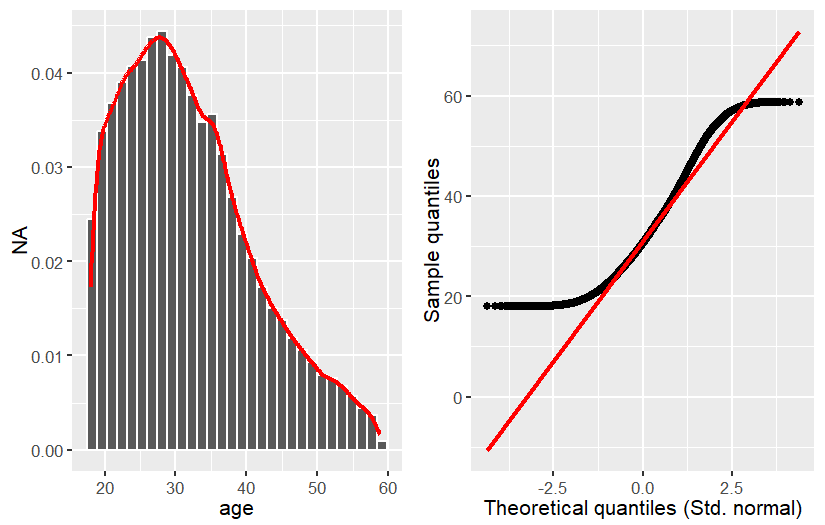
\includegraphics{qmd/appendice-chapter-4_files/figure-pdf/unnamed-chunk-5-1.png}

\legend{Source: Created by the author.}

}

\end{figure}%

\begin{Shaded}
\begin{Highlighting}[numbers=left,,]
\NormalTok{stats}\SpecialCharTok{$}\NormalTok{stats }\SpecialCharTok{|\textgreater{}} \FunctionTok{list\_as\_tibble}\NormalTok{()}
\end{Highlighting}
\end{Shaded}

\begin{table}

\caption{\label{tbl-appendice-chapter-4-distribution-of-main-variables}Statistics
related to the \(\text{age}\) variable.}

\centering{

\begin{longtable}[]{@{}ll@{}}
\toprule\noalign{}
name & value \\
\midrule\noalign{}
\endhead
\bottomrule\noalign{}
\endlastfoot
n & 79198 \\
n\_rm\_na & 79198 \\
n\_na & 0 \\
mean & 31.9838074965417 \\
var & 85.2414919292643 \\
sd & 9.23263190695179 \\
min & 18 \\
q\_1 & 24.7222222222222 \\
median & 30.5388888888889 \\
q\_3 & 37.61875 \\
max & 58.7861111111111 \\
iqr & 12.8965277777778 \\
skewness & 0.665751526654394 \\
kurtosis & 2.82381488030798 \\
\end{longtable}

\addtocounter{table}{-1}

\legend{Source: Created by the author.}

}

\end{table}%

\section{Geographic distribution}\label{geographic-distribution}

\begin{Shaded}
\begin{Highlighting}[numbers=left,,]
\FunctionTok{source}\NormalTok{(here}\SpecialCharTok{::}\FunctionTok{here}\NormalTok{(}\StringTok{"R/plot\_brazil\_uf\_map.R"}\NormalTok{))}

\NormalTok{rutils}\SpecialCharTok{:::}\FunctionTok{assert\_internet}\NormalTok{()}

\NormalTok{brazil\_uf\_map }\OtherTok{\textless{}{-}} 
\NormalTok{  data }\SpecialCharTok{|\textgreater{}} 
  \FunctionTok{plot\_brazil\_uf\_map}\NormalTok{(}\AttributeTok{option =} \StringTok{"viridis"}\NormalTok{, }\AttributeTok{text\_size =}\NormalTok{ env\_vars}\SpecialCharTok{$}\NormalTok{base\_size)}
\end{Highlighting}
\end{Shaded}

\begin{figure}[H]

\caption{\label{fig-appendice-chapter-4-geographic-distribution}Geographic
distribution of the sample subjects.}

\centering{

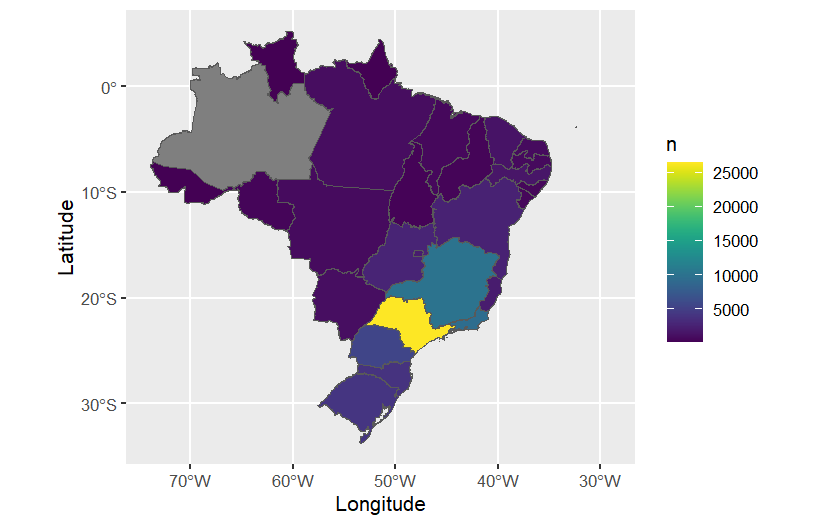
\includegraphics{qmd/appendice-chapter-4_files/figure-pdf/unnamed-chunk-7-1.png}

\legend{Source: Created by the author.}

}

\end{figure}%

\section{Age pyramid}\label{age-pyramid}

\begin{Shaded}
\begin{Highlighting}[numbers=left,,]
\FunctionTok{source}\NormalTok{(here}\SpecialCharTok{::}\FunctionTok{here}\NormalTok{(}\StringTok{"R/plot\_age\_pyramid.R"}\NormalTok{))}

\NormalTok{age\_pyramid }\OtherTok{\textless{}{-}} 
\NormalTok{  data }\SpecialCharTok{|\textgreater{}} 
  \FunctionTok{plot\_age\_pyramid}\NormalTok{(}
    \AttributeTok{interval =} \DecValTok{10}\NormalTok{, }
    \AttributeTok{na\_rm =} \ConstantTok{TRUE}\NormalTok{, }
    \AttributeTok{text\_size =}\NormalTok{ env\_vars}\SpecialCharTok{$}\NormalTok{base\_size}
\NormalTok{  )}
\end{Highlighting}
\end{Shaded}

\begin{figure}[H]

\caption{\label{fig-appendice-chapter-4-age-pyramid}Age pyramid of the
sample subjects.}

\centering{

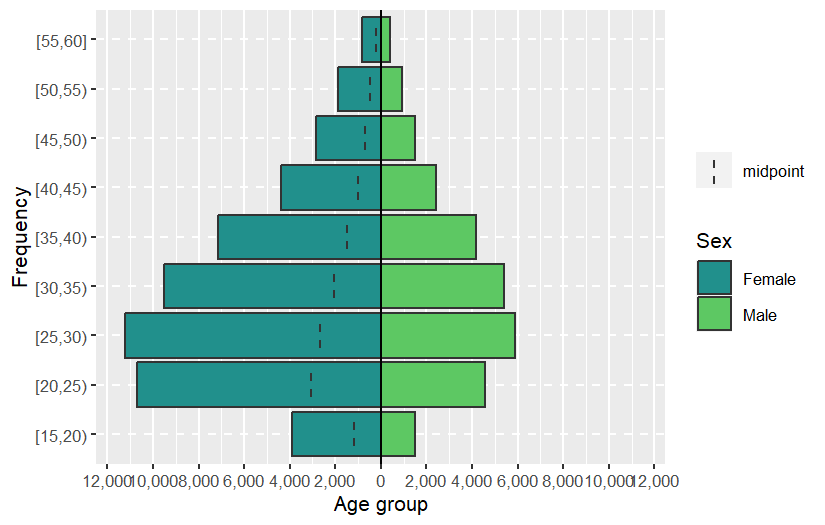
\includegraphics{qmd/appendice-chapter-4_files/figure-pdf/unnamed-chunk-8-1.png}

\legend{Source: Created by the author.}

}

\end{figure}%

\section{Correlation matrix}\label{correlation-matrix}

\begin{Shaded}
\begin{Highlighting}[numbers=left,,]
\FunctionTok{source}\NormalTok{(here}\SpecialCharTok{::}\FunctionTok{here}\NormalTok{(}\StringTok{"R/plot\_ggcorrplot.R"}\NormalTok{))}

\NormalTok{cols }\OtherTok{\textless{}{-}} \FunctionTok{c}\NormalTok{(}\StringTok{"sex"}\NormalTok{, }\StringTok{"age"}\NormalTok{, }\StringTok{"latitude"}\NormalTok{, }\StringTok{"longitude"}\NormalTok{, }\StringTok{"msf\_sc"}\NormalTok{, }\StringTok{"sjl"}\NormalTok{, }\StringTok{"le\_week"}\NormalTok{)}

\NormalTok{ggcorrplot }\OtherTok{\textless{}{-}}
\NormalTok{  data }\SpecialCharTok{|\textgreater{}}
  \FunctionTok{plot\_ggcorrplot}\NormalTok{(}
    \AttributeTok{cols =}\NormalTok{ cols, }
    \AttributeTok{na\_rm =} \ConstantTok{TRUE}\NormalTok{, }
    \AttributeTok{text\_size =}\NormalTok{ env\_vars}\SpecialCharTok{$}\NormalTok{base\_size, }
    \AttributeTok{hc\_order =} \ConstantTok{TRUE}
\NormalTok{    )}
\end{Highlighting}
\end{Shaded}

\begin{figure}[H]

\caption{\label{fig-appendice-chapter-4-correlation-matrix}Correlation
matrix of the main variables.}

\centering{

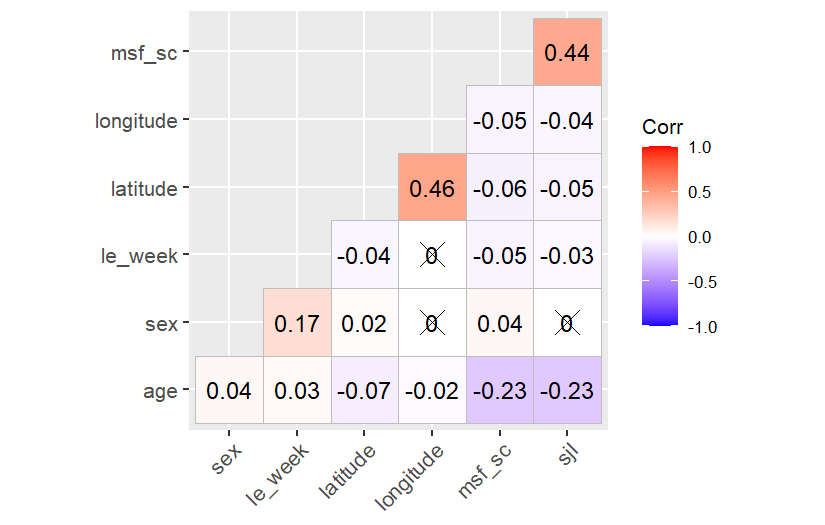
\includegraphics{qmd/appendice-chapter-4_files/figure-pdf/unnamed-chunk-10-1.png}

\legend{Source: Created by the author.}

}

\end{figure}%

\section{Age and sex series}\label{age-and-sex-series}

\subsection{\texorpdfstring{Age/sex \emph{versus}
chronotype}{Age/sex versus chronotype}}\label{agesex-versus-chronotype}

\begin{Shaded}
\begin{Highlighting}[numbers=left,,]
\FunctionTok{source}\NormalTok{(here}\SpecialCharTok{::}\FunctionTok{here}\NormalTok{(}\StringTok{"R/plot\_age\_series.R"}\NormalTok{))}

\NormalTok{col }\OtherTok{\textless{}{-}} \StringTok{"msf\_sc"}
\NormalTok{y\_lab }\OtherTok{\textless{}{-}}\NormalTok{ latex2exp}\SpecialCharTok{::}\FunctionTok{TeX}\NormalTok{(}\StringTok{"Local time ($MSF\_\{sc\}$)"}\NormalTok{)}

\NormalTok{data }\SpecialCharTok{|\textgreater{}}
\NormalTok{  dplyr}\SpecialCharTok{::}\FunctionTok{filter}\NormalTok{(age }\SpecialCharTok{\textless{}=} \DecValTok{50}\NormalTok{) }\SpecialCharTok{|\textgreater{}}
  \FunctionTok{plot\_age\_series}\NormalTok{(}
    \AttributeTok{col =}\NormalTok{ col, }
    \AttributeTok{y\_lab =}\NormalTok{ y\_lab, }
    \AttributeTok{line\_width =} \DecValTok{2}\NormalTok{, }
    \AttributeTok{boundary =} \FloatTok{0.5}\NormalTok{, }
    \AttributeTok{point\_size =} \DecValTok{1}\NormalTok{,}
    \AttributeTok{error\_bar\_width =} \FloatTok{0.5}\NormalTok{, }
    \AttributeTok{error\_bar\_linewidth =} \FloatTok{0.5}\NormalTok{, }
    \AttributeTok{error\_bar =} \ConstantTok{TRUE}\NormalTok{,}
    \AttributeTok{text\_size =}\NormalTok{ env\_vars}\SpecialCharTok{$}\NormalTok{base\_size}
\NormalTok{    )}
\end{Highlighting}
\end{Shaded}

\begin{figure}[H]

\caption{\label{fig-appendice-chapter-4-age-sex-chronotype-series}Relation
between age and chronotype, divided by sex. Chronotype is represented by
the local time of the midpoint between sleep onset and sleep end on
work-free days (\(\text{MSF}_{\text{sc}}\)), MCTQ proxy for measuring
the chronotype. The gray line represents both sex. Vertical lines
represent the standard error of the mean (SEM).}

\centering{

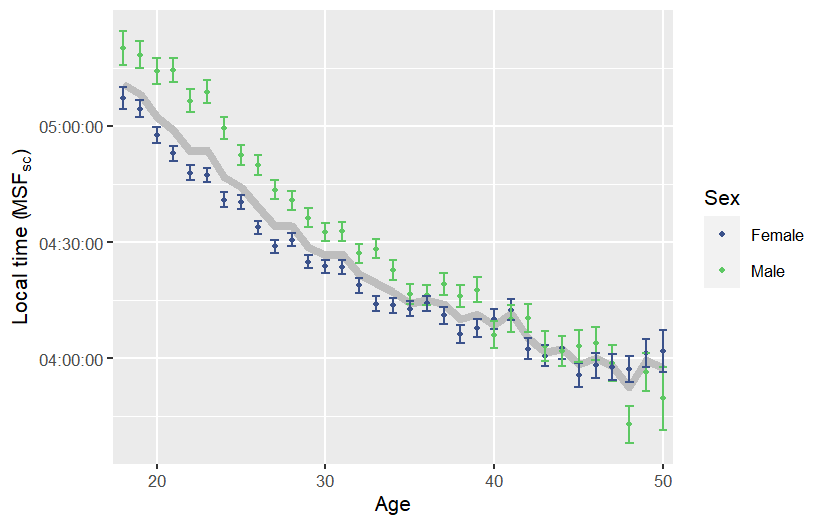
\includegraphics{qmd/appendice-chapter-4_files/figure-pdf/unnamed-chunk-11-1.png}

\legend{Source: Created by the author. Based on the data visualization
found in \textcite{roenneberg2007a}.}

}

\end{figure}%

\subsection{\texorpdfstring{Age/sex \emph{versus}
weight}{Age/sex versus weight}}\label{agesex-versus-weight}

\begin{Shaded}
\begin{Highlighting}[numbers=left,,]
\FunctionTok{source}\NormalTok{(here}\SpecialCharTok{::}\FunctionTok{here}\NormalTok{(}\StringTok{"R/plot\_age\_series.R"}\NormalTok{))}

\NormalTok{col }\OtherTok{\textless{}{-}} \StringTok{"weight"}
\NormalTok{y\_lab }\OtherTok{\textless{}{-}} \StringTok{"Weight (kg)"}

\NormalTok{data }\SpecialCharTok{|\textgreater{}}
\NormalTok{  dplyr}\SpecialCharTok{::}\FunctionTok{filter}\NormalTok{(age }\SpecialCharTok{\textless{}=} \DecValTok{50}\NormalTok{) }\SpecialCharTok{|\textgreater{}}
  \FunctionTok{plot\_age\_series}\NormalTok{(}
    \AttributeTok{col =}\NormalTok{ col, }
    \AttributeTok{y\_lab =}\NormalTok{ y\_lab, }
    \AttributeTok{line\_width =} \DecValTok{2}\NormalTok{, }
    \AttributeTok{boundary =} \FloatTok{0.5}\NormalTok{, }
    \AttributeTok{point\_size =} \DecValTok{1}\NormalTok{,}
    \AttributeTok{error\_bar\_width =} \FloatTok{0.5}\NormalTok{, }
    \AttributeTok{error\_bar\_linewidth =} \FloatTok{0.5}\NormalTok{, }
    \AttributeTok{error\_bar =} \ConstantTok{TRUE}\NormalTok{,}
    \AttributeTok{text\_size =}\NormalTok{ env\_vars}\SpecialCharTok{$}\NormalTok{base\_size}
\NormalTok{    )}
\end{Highlighting}
\end{Shaded}

\begin{figure}[H]

\caption{\label{fig-appendice-chapter-4-age-sex-weight-series}Relation
between age and weight (kg), divided by sex. The gray line represents
both sex. Vertical lines represent the standard error of the mean
(SEM).}

\centering{

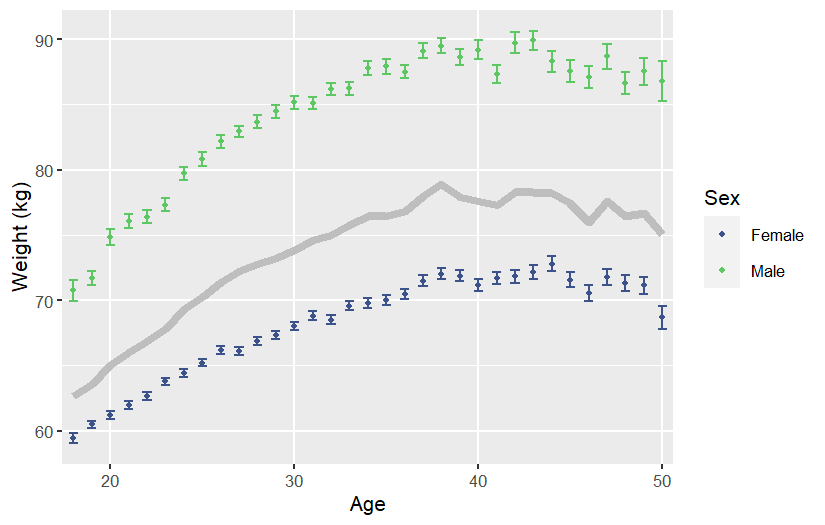
\includegraphics{qmd/appendice-chapter-4_files/figure-pdf/unnamed-chunk-12-1.png}

\legend{Source: Created by the author. Based on the data visualization
found in \textcite{roenneberg2007a}.}

}

\end{figure}%

\section{Chronotype distribution}\label{chronotype-distribution}

\begin{Shaded}
\begin{Highlighting}[numbers=left,,]
\FunctionTok{source}\NormalTok{(here}\SpecialCharTok{::}\FunctionTok{here}\NormalTok{(}\StringTok{"R/plot\_chronotype.R"}\NormalTok{))}

\NormalTok{col }\OtherTok{\textless{}{-}} \StringTok{"msf\_sc"}
\NormalTok{y\_lab }\OtherTok{\textless{}{-}}\NormalTok{ latex2exp}\SpecialCharTok{::}\FunctionTok{TeX}\NormalTok{(}\StringTok{"Local time ($MSF\_\{sc\}$)"}\NormalTok{)}

\NormalTok{data }\SpecialCharTok{|\textgreater{}}
  \FunctionTok{plot\_chronotype}\NormalTok{(}
    \AttributeTok{col =}\NormalTok{ col, }
    \AttributeTok{x\_lab =} \StringTok{"Frequency (\%)"}\NormalTok{,}
    \AttributeTok{y\_lab =}\NormalTok{ y\_lab,}
    \AttributeTok{col\_width =} \FloatTok{0.8}\NormalTok{, }
    \AttributeTok{col\_border =} \FloatTok{0.6}\NormalTok{, }
    \AttributeTok{text\_size =}\NormalTok{ env\_vars}\SpecialCharTok{$}\NormalTok{base\_size,}
    \AttributeTok{legend\_position =} \StringTok{"right"}\NormalTok{,}
    \AttributeTok{chronotype\_cuts =} \ConstantTok{FALSE}
\NormalTok{  )}
\end{Highlighting}
\end{Shaded}

\begin{figure}[H]

\caption{\label{fig-appendice-chapter-4-chronotype-distribution}Distribution
of the local time of the midpoint between sleep onset and sleep end on
work-free days (\(\text{MSF}_{\text{sc}}\)), MCTQ proxy for measuring
the chronotype. The categorical cuts follow a quantile approach going
from extremely early (\(0 |- 0.11\)) to the extremely late
(\(0.88 - 1\)).}

\centering{

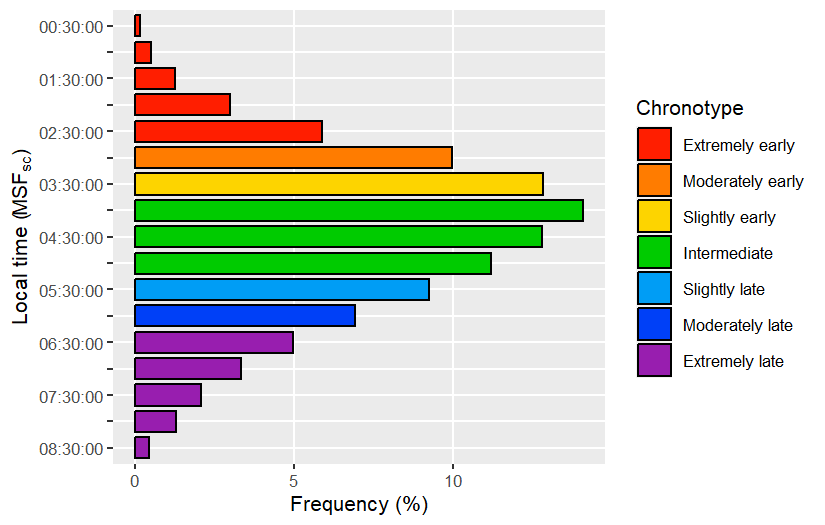
\includegraphics{qmd/appendice-chapter-4_files/figure-pdf/unnamed-chunk-13-1.png}

\legend{Source: Created by the author. Based on the data visualization
found in \textcite{roenneberg2019b}.}

}

\end{figure}%

\section{Latitude series}\label{latitude-series}

\begin{Shaded}
\begin{Highlighting}[numbers=left,,]
\FunctionTok{source}\NormalTok{(here}\SpecialCharTok{::}\FunctionTok{here}\NormalTok{(}\StringTok{"R/plot\_latitude\_series.R"}\NormalTok{))}

\NormalTok{col }\OtherTok{\textless{}{-}} \StringTok{"msf\_sc"}
\NormalTok{y\_lab }\OtherTok{\textless{}{-}}\NormalTok{ latex2exp}\SpecialCharTok{::}\FunctionTok{TeX}\NormalTok{(}\StringTok{"$MSF\_\{sc\} }\SpecialCharTok{\textbackslash{}\textbackslash{}}\StringTok{pm SEM$"}\NormalTok{)}

\NormalTok{data }\SpecialCharTok{|\textgreater{}}
\NormalTok{  dplyr}\SpecialCharTok{::}\FunctionTok{filter}\NormalTok{(age }\SpecialCharTok{\textless{}=} \DecValTok{50}\NormalTok{) }\SpecialCharTok{|\textgreater{}}
  \FunctionTok{plot\_latitude\_series}\NormalTok{(}
    \AttributeTok{col =}\NormalTok{ col, }
    \AttributeTok{y\_lab =}\NormalTok{ y\_lab, }
    \AttributeTok{line\_width =} \DecValTok{2}\NormalTok{, }
    \AttributeTok{point\_size =} \DecValTok{3}\NormalTok{,}
    \AttributeTok{error\_bar\_width =} \FloatTok{0.5}\NormalTok{, }
    \AttributeTok{error\_bar\_linewidth =} \DecValTok{1}\NormalTok{, }
    \AttributeTok{error\_bar =} \ConstantTok{TRUE}\NormalTok{,}
    \AttributeTok{text\_size =}\NormalTok{ env\_vars}\SpecialCharTok{$}\NormalTok{base\_size}
\NormalTok{  )}
\end{Highlighting}
\end{Shaded}

\begin{figure}[H]

\caption{\label{fig-appendice-chapter-4-latitude-series}Distribution of
mean aggregates of the local time of the midpoint between sleep onset
and sleep end on work-free days (\(\text{MSF}_{\text{sc}}\)), MCTQ proxy
for measuring the chronotype, in relation to latitude decimal degree
intervals. Higher values of \(\text{MSF}_{\text{sc}}\) indicate a
tendency toward a late chronotype. The red line represents a linear
regression, and the shaded area indicates a pointwise 95\% confidence
interval.}

\centering{

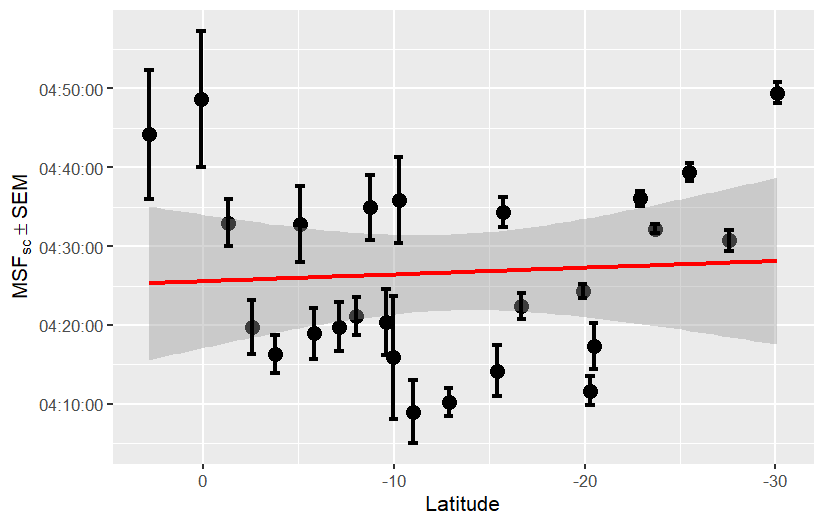
\includegraphics{qmd/appendice-chapter-4_files/figure-pdf/unnamed-chunk-14-1.png}

\legend{Source: Created by the author. Based on the data visualization
found in \textcite{leocadio-miguel2017}.}

}

\end{figure}%

\section{Statistics}\label{statistics}

\subsection{Numerical variables}\label{numerical-variables}

\begin{Shaded}
\begin{Highlighting}[numbers=left,,]
\FunctionTok{source}\NormalTok{(here}\SpecialCharTok{::}\FunctionTok{here}\NormalTok{(}\StringTok{"R/stats\_sum.R"}\NormalTok{))}
\FunctionTok{source}\NormalTok{(here}\SpecialCharTok{::}\FunctionTok{here}\NormalTok{(}\StringTok{"R/utils.R"}\NormalTok{))}

\NormalTok{col }\OtherTok{\textless{}{-}} \StringTok{"msf\_sc"}

\NormalTok{data }\SpecialCharTok{|\textgreater{}}
\NormalTok{  magrittr}\SpecialCharTok{::}\FunctionTok{extract2}\NormalTok{(col) }\SpecialCharTok{|\textgreater{}}
  \FunctionTok{stats\_sum}\NormalTok{(}\AttributeTok{print =} \ConstantTok{FALSE}\NormalTok{) }\SpecialCharTok{|\textgreater{}}
  \FunctionTok{list\_as\_tibble}\NormalTok{()}
\end{Highlighting}
\end{Shaded}

\begin{table}

\caption{\label{tbl-appendice-chapter-4-statistics-numerical-variables}Statistics
related to the MSF\textsubscript{sc} variable.}

\centering{

\begin{longtable}[]{@{}ll@{}}
\toprule\noalign{}
name & value \\
\midrule\noalign{}
\endhead
\bottomrule\noalign{}
\endlastfoot
n & 79198 \\
n\_rm\_na & 79198 \\
n\_na & 0 \\
mean & 04:28:17.770957 \\
var & 08:05:53.49992 \\
sd & 01:26:51.406096 \\
min & 00:22:30 \\
q\_1 & 03:26:25.714286 \\
median & 04:20:42.857143 \\
q\_3 & 05:25:42.857143 \\
max & 08:31:04.285714 \\
iqr & 01:59:17.142857 \\
skewness & 0.284586184927996 \\
kurtosis & 2.77321491178072 \\
\end{longtable}

\addtocounter{table}{-1}

\legend{Source: Created by the author.}

}

\end{table}%

\subsection{Sex}\label{sex}

\begin{Shaded}
\begin{Highlighting}[numbers=left,,]
\CommentTok{\# See \textless{}https://sidra.ibge.gov.br\textgreater{} to learn more.}

\FunctionTok{library}\NormalTok{(magrittr)}

\NormalTok{rutils}\SpecialCharTok{:::}\FunctionTok{assert\_internet}\NormalTok{()}

\CommentTok{\# Brazil\textquotesingle{}s 2022 census data}
\NormalTok{census\_data }\OtherTok{\textless{}{-}} 
\NormalTok{  sidrar}\SpecialCharTok{::}\FunctionTok{get\_sidra}\NormalTok{(}\AttributeTok{x =} \DecValTok{9514}\NormalTok{) }\SpecialCharTok{\%\textgreater{}\%} \CommentTok{\# Don\textquotesingle{}t change the pipe}
\NormalTok{  dplyr}\SpecialCharTok{::}\FunctionTok{filter}\NormalTok{(}
\NormalTok{    Sexo }\SpecialCharTok{\%in\%} \FunctionTok{c}\NormalTok{(}\StringTok{"Homens"}\NormalTok{, }\StringTok{"Mulheres"}\NormalTok{, }\StringTok{"Total"}\NormalTok{),}
\NormalTok{    stringr}\SpecialCharTok{::}\FunctionTok{str\_detect}\NormalTok{(}
\NormalTok{      Idade, }
      \StringTok{"\^{}(1[8{-}9]|[2{-}9][0{-}9]) (ano|anos)$|\^{}100 anos ou mais$"}
\NormalTok{    ),}
\NormalTok{    .[[}\DecValTok{17}\NormalTok{]] }\SpecialCharTok{==} \StringTok{"Total"}
\NormalTok{    ) }\SpecialCharTok{|\textgreater{}}
\NormalTok{  dplyr}\SpecialCharTok{::}\FunctionTok{transmute}\NormalTok{(}
    \AttributeTok{sex =}\NormalTok{ dplyr}\SpecialCharTok{::}\FunctionTok{case\_when}\NormalTok{(}
\NormalTok{      Sexo }\SpecialCharTok{==} \StringTok{"Homens"} \SpecialCharTok{\textasciitilde{}} \StringTok{"Male"}\NormalTok{,}
\NormalTok{      Sexo }\SpecialCharTok{==} \StringTok{"Mulheres"} \SpecialCharTok{\textasciitilde{}} \StringTok{"Female"}\NormalTok{,}
\NormalTok{      Sexo }\SpecialCharTok{==} \StringTok{"Total"} \SpecialCharTok{\textasciitilde{}} \StringTok{"Total"}
\NormalTok{    ),}
    \AttributeTok{value =}\NormalTok{ Valor}
\NormalTok{  ) }\SpecialCharTok{|\textgreater{}}
\NormalTok{  dplyr}\SpecialCharTok{::}\FunctionTok{group\_by}\NormalTok{(sex) }\SpecialCharTok{|\textgreater{}}
\NormalTok{  dplyr}\SpecialCharTok{::}\FunctionTok{summarise}\NormalTok{(}\AttributeTok{n =} \FunctionTok{sum}\NormalTok{(value)) }\SpecialCharTok{|\textgreater{}}
\NormalTok{  dplyr}\SpecialCharTok{::}\FunctionTok{ungroup}\NormalTok{()}

\NormalTok{census\_data }\OtherTok{\textless{}{-}} 
\NormalTok{  dplyr}\SpecialCharTok{::}\FunctionTok{bind\_rows}\NormalTok{(}
\NormalTok{    census\_data }\SpecialCharTok{|\textgreater{}}
\NormalTok{      dplyr}\SpecialCharTok{::}\FunctionTok{filter}\NormalTok{(sex }\SpecialCharTok{!=} \StringTok{"Total"}\NormalTok{) }\SpecialCharTok{|\textgreater{}}
\NormalTok{      dplyr}\SpecialCharTok{::}\FunctionTok{mutate}\NormalTok{(}
        \AttributeTok{n\_rel =}\NormalTok{ n }\SpecialCharTok{/} \FunctionTok{sum}\NormalTok{(n[sex }\SpecialCharTok{!=} \StringTok{"Total"}\NormalTok{]),}
        \AttributeTok{n\_per =} \FunctionTok{round}\NormalTok{(n\_rel }\SpecialCharTok{*} \DecValTok{100}\NormalTok{, }\DecValTok{3}\NormalTok{)}
\NormalTok{      ),}
\NormalTok{    census\_data }\SpecialCharTok{|\textgreater{}}
\NormalTok{      dplyr}\SpecialCharTok{::}\FunctionTok{filter}\NormalTok{(sex }\SpecialCharTok{==} \StringTok{"Total"}\NormalTok{) }\SpecialCharTok{|\textgreater{}}
\NormalTok{      dplyr}\SpecialCharTok{::}\FunctionTok{mutate}\NormalTok{(}\AttributeTok{n\_rel =} \DecValTok{1}\NormalTok{, }\AttributeTok{n\_per =} \DecValTok{100}\NormalTok{)}
\NormalTok{  ) }\SpecialCharTok{|\textgreater{}}
\NormalTok{  dplyr}\SpecialCharTok{::}\FunctionTok{as\_tibble}\NormalTok{() }\SpecialCharTok{|\textgreater{}}
\NormalTok{  dplyr}\SpecialCharTok{::}\FunctionTok{arrange}\NormalTok{(sex)}

\NormalTok{count }\OtherTok{\textless{}{-}}\NormalTok{ data }\SpecialCharTok{|\textgreater{}}
\NormalTok{  dplyr}\SpecialCharTok{::}\FunctionTok{select}\NormalTok{(sex) }\SpecialCharTok{|\textgreater{}}
\NormalTok{  dplyr}\SpecialCharTok{::}\FunctionTok{group\_by}\NormalTok{(sex) }\SpecialCharTok{|\textgreater{}}
\NormalTok{  dplyr}\SpecialCharTok{::}\FunctionTok{summarise}\NormalTok{(}\AttributeTok{n =}\NormalTok{ dplyr}\SpecialCharTok{::}\FunctionTok{n}\NormalTok{()) }\SpecialCharTok{|\textgreater{}}
\NormalTok{  dplyr}\SpecialCharTok{::}\FunctionTok{ungroup}\NormalTok{() }\SpecialCharTok{|\textgreater{}}
\NormalTok{  dplyr}\SpecialCharTok{::}\FunctionTok{mutate}\NormalTok{(}
    \AttributeTok{n\_rel =}\NormalTok{ n }\SpecialCharTok{/} \FunctionTok{sum}\NormalTok{(n),}
    \AttributeTok{n\_per =} \FunctionTok{round}\NormalTok{(n\_rel }\SpecialCharTok{*} \DecValTok{100}\NormalTok{, }\DecValTok{3}\NormalTok{)}
\NormalTok{  ) }\SpecialCharTok{|\textgreater{}}
\NormalTok{  dplyr}\SpecialCharTok{::}\FunctionTok{arrange}\NormalTok{(dplyr}\SpecialCharTok{::}\FunctionTok{desc}\NormalTok{(n\_rel)) }\SpecialCharTok{|\textgreater{}}
\NormalTok{  dplyr}\SpecialCharTok{::}\FunctionTok{bind\_rows}\NormalTok{(}
\NormalTok{    dplyr}\SpecialCharTok{::}\FunctionTok{tibble}\NormalTok{(}
      \AttributeTok{sex =} \StringTok{"Total"}\NormalTok{,}
      \AttributeTok{n =} \FunctionTok{nrow}\NormalTok{(tidyr}\SpecialCharTok{::}\FunctionTok{drop\_na}\NormalTok{(data, sex)),}
      \AttributeTok{n\_rel =} \DecValTok{1}\NormalTok{, }
      \AttributeTok{n\_per =} \DecValTok{100}
\NormalTok{    )}
\NormalTok{  )}

\NormalTok{count }\OtherTok{\textless{}{-}} 
\NormalTok{  dplyr}\SpecialCharTok{::}\FunctionTok{left\_join}\NormalTok{(}
\NormalTok{    count, census\_data, }
    \AttributeTok{by =} \StringTok{"sex"}\NormalTok{, }
    \AttributeTok{suffix =} \FunctionTok{c}\NormalTok{(}\StringTok{"\_sample"}\NormalTok{, }\StringTok{"\_census"}\NormalTok{)}
\NormalTok{  ) }\SpecialCharTok{|\textgreater{}}
\NormalTok{  dplyr}\SpecialCharTok{::}\FunctionTok{mutate}\NormalTok{(}
    \AttributeTok{n\_rel\_diff =}\NormalTok{ n\_rel\_sample }\SpecialCharTok{{-}}\NormalTok{ n\_rel\_census,}
    \AttributeTok{n\_per\_diff =}\NormalTok{ n\_per\_sample }\SpecialCharTok{{-}}\NormalTok{ n\_per\_census}
\NormalTok{  ) }\SpecialCharTok{|\textgreater{}}
\NormalTok{  dplyr}\SpecialCharTok{::}\FunctionTok{relocate}\NormalTok{(}
\NormalTok{    sex, n\_sample, n\_census, n\_rel\_sample, n\_rel\_census, n\_rel\_diff,}
\NormalTok{    n\_per\_sample, n\_per\_census, n\_per\_diff}
\NormalTok{  )}

\NormalTok{count }\SpecialCharTok{|\textgreater{}}\NormalTok{ dplyr}\SpecialCharTok{::}\FunctionTok{select}\NormalTok{(sex, n\_per\_sample, n\_per\_census, n\_per\_diff)}
\end{Highlighting}
\end{Shaded}

\begin{table}

\caption{\label{tbl-appendice-chapter-4-statistics-sex-1}Frequencies of
sex among subjects compared with data from Brazil's 2022 census.}

\centering{

\begin{longtable}[]{@{}lrrr@{}}
\toprule\noalign{}
sex & n\_per\_sample & n\_per\_census & n\_per\_diff \\
\midrule\noalign{}
\endhead
\bottomrule\noalign{}
\endlastfoot
Female & 66.243 & 52.263 & 13.98 \\
Male & 33.757 & 47.737 & -13.98 \\
Total & 100.000 & 100.000 & 0.00 \\
\end{longtable}

\addtocounter{table}{-1}

\legend{Source: Created by the author, based on data from Brazil's 2022
census (\textcite{ibgeb}).}

}

\end{table}%

\begin{Shaded}
\begin{Highlighting}[numbers=left,,]
\FunctionTok{sum}\NormalTok{(count}\SpecialCharTok{$}\NormalTok{n\_per\_diff)}
\CommentTok{\#\textgreater{} [1] {-}7.105427e{-}15}
\end{Highlighting}
\end{Shaded}

\subsection{Age and sex}\label{age-and-sex}

\begin{Shaded}
\begin{Highlighting}[numbers=left,,]
\FunctionTok{source}\NormalTok{(here}\SpecialCharTok{::}\FunctionTok{here}\NormalTok{(}\StringTok{"R/stats\_sum.R"}\NormalTok{))}
\FunctionTok{source}\NormalTok{(here}\SpecialCharTok{::}\FunctionTok{here}\NormalTok{(}\StringTok{"R/utils.R"}\NormalTok{))}

\NormalTok{value }\OtherTok{\textless{}{-}} \StringTok{"Male"}

\NormalTok{data }\SpecialCharTok{|\textgreater{}}
\NormalTok{  dplyr}\SpecialCharTok{::}\FunctionTok{filter}\NormalTok{(sex }\SpecialCharTok{==}\NormalTok{ value) }\SpecialCharTok{|\textgreater{}}
\NormalTok{  magrittr}\SpecialCharTok{::}\FunctionTok{extract2}\NormalTok{(}\StringTok{"age"}\NormalTok{) }\SpecialCharTok{|\textgreater{}}
  \FunctionTok{stats\_sum}\NormalTok{(}\AttributeTok{print =} \ConstantTok{FALSE}\NormalTok{) }\SpecialCharTok{|\textgreater{}}
  \FunctionTok{list\_as\_tibble}\NormalTok{()}
\end{Highlighting}
\end{Shaded}

\begin{table}

\caption{\label{tbl-appendice-chapter-4-statistics-sex-age-1}Statistics
related to male subject's age.}

\centering{

\begin{longtable}[]{@{}ll@{}}
\toprule\noalign{}
name & value \\
\midrule\noalign{}
\endhead
\bottomrule\noalign{}
\endlastfoot
n & 26735 \\
n\_rm\_na & 26735 \\
n\_na & 0 \\
mean & 32.4343759740665 \\
var & 80.9906211885464 \\
sd & 8.99947893983571 \\
min & 18 \\
q\_1 & 25.5388888888889 \\
median & 31.2583333333333 \\
q\_3 & 37.9319444444444 \\
max & 58.7722222222222 \\
iqr & 12.3930555555556 \\
skewness & 0.617696405622681 \\
kurtosis & 2.84390555184727 \\
\end{longtable}

\addtocounter{table}{-1}

\legend{Source: Created by the author.}

}

\end{table}%

\begin{Shaded}
\begin{Highlighting}[numbers=left,,]
\CommentTok{\# See \textless{}https://sidra.ibge.gov.br\textgreater{} to learn more.}

\FunctionTok{library}\NormalTok{(magrittr)}

\NormalTok{rutils}\SpecialCharTok{:::}\FunctionTok{assert\_internet}\NormalTok{()}

\CommentTok{\# Brazil\textquotesingle{}s 2022 census data}
\NormalTok{census\_data }\OtherTok{\textless{}{-}} 
\NormalTok{  sidrar}\SpecialCharTok{::}\FunctionTok{get\_sidra}\NormalTok{(}\AttributeTok{x =} \DecValTok{9514}\NormalTok{) }\SpecialCharTok{\%\textgreater{}\%} \CommentTok{\# Don\textquotesingle{}t change the pipe}
\NormalTok{  dplyr}\SpecialCharTok{::}\FunctionTok{filter}\NormalTok{(}
\NormalTok{    Sexo }\SpecialCharTok{\%in\%} \FunctionTok{c}\NormalTok{(}\StringTok{"Homens"}\NormalTok{, }\StringTok{"Mulheres"}\NormalTok{, }\StringTok{"Total"}\NormalTok{),}
\NormalTok{    stringr}\SpecialCharTok{::}\FunctionTok{str\_detect}\NormalTok{(}
\NormalTok{      Idade, }
      \StringTok{"\^{}(1[8{-}9]|[2{-}9][0{-}9]) (ano|anos)$|\^{}100 anos ou mais$"}
\NormalTok{    ),}
\NormalTok{    .[[}\DecValTok{17}\NormalTok{]] }\SpecialCharTok{==} \StringTok{"Total"}
\NormalTok{    ) }\SpecialCharTok{|\textgreater{}}
\NormalTok{  dplyr}\SpecialCharTok{::}\FunctionTok{transmute}\NormalTok{(}
    \AttributeTok{sex =}\NormalTok{ dplyr}\SpecialCharTok{::}\FunctionTok{case\_when}\NormalTok{(}
\NormalTok{      Sexo }\SpecialCharTok{==} \StringTok{"Homens"} \SpecialCharTok{\textasciitilde{}} \StringTok{"Male"}\NormalTok{,}
\NormalTok{      Sexo }\SpecialCharTok{==} \StringTok{"Mulheres"} \SpecialCharTok{\textasciitilde{}} \StringTok{"Female"}\NormalTok{,}
\NormalTok{      Sexo }\SpecialCharTok{==} \StringTok{"Total"} \SpecialCharTok{\textasciitilde{}} \StringTok{"Total"}
\NormalTok{    ),}
    \AttributeTok{age =} \FunctionTok{as.numeric}\NormalTok{(stringr}\SpecialCharTok{::}\FunctionTok{str\_extract}\NormalTok{(Idade, }\StringTok{"}\SpecialCharTok{\textbackslash{}\textbackslash{}}\StringTok{d+"}\NormalTok{)),}
    \AttributeTok{value =}\NormalTok{ Valor}
\NormalTok{  ) }\SpecialCharTok{|\textgreater{}}
\NormalTok{  dplyr}\SpecialCharTok{::}\FunctionTok{group\_by}\NormalTok{(sex) }\SpecialCharTok{|\textgreater{}}
\NormalTok{  dplyr}\SpecialCharTok{::}\FunctionTok{summarise}\NormalTok{(}
    \AttributeTok{mean =}\NormalTok{ stats}\SpecialCharTok{::}\FunctionTok{weighted.mean}\NormalTok{(age, value),}
    \AttributeTok{sd =} \FunctionTok{sqrt}\NormalTok{(Hmisc}\SpecialCharTok{::}\FunctionTok{wtd.var}\NormalTok{(age, value))}
\NormalTok{  ) }\SpecialCharTok{|\textgreater{}} 
\NormalTok{  dplyr}\SpecialCharTok{::}\FunctionTok{ungroup}\NormalTok{() }\SpecialCharTok{|\textgreater{}}
\NormalTok{  dplyr}\SpecialCharTok{::}\FunctionTok{mutate}\NormalTok{(}
    \AttributeTok{min =} \FunctionTok{c}\NormalTok{(}\DecValTok{18}\NormalTok{, }\DecValTok{18}\NormalTok{, }\DecValTok{18}\NormalTok{),}
    \AttributeTok{max =} \FunctionTok{c}\NormalTok{(}\DecValTok{100}\NormalTok{, }\DecValTok{100}\NormalTok{, }\DecValTok{100}\NormalTok{)}
\NormalTok{  ) }\SpecialCharTok{|\textgreater{}}
\NormalTok{  dplyr}\SpecialCharTok{::}\FunctionTok{relocate}\NormalTok{(sex, mean, sd, min, max) }\SpecialCharTok{|\textgreater{}}
\NormalTok{  dplyr}\SpecialCharTok{::}\FunctionTok{as\_tibble}\NormalTok{()}

\NormalTok{count }\OtherTok{\textless{}{-}}\NormalTok{ data }\SpecialCharTok{|\textgreater{}}
\NormalTok{  dplyr}\SpecialCharTok{::}\FunctionTok{select}\NormalTok{(sex, age) }\SpecialCharTok{|\textgreater{}}
\NormalTok{  dplyr}\SpecialCharTok{::}\FunctionTok{group\_by}\NormalTok{(sex) }\SpecialCharTok{|\textgreater{}}
\NormalTok{  dplyr}\SpecialCharTok{::}\FunctionTok{mutate}\NormalTok{(}\AttributeTok{sex =} \FunctionTok{as.character}\NormalTok{(sex)) }\SpecialCharTok{|\textgreater{}}
\NormalTok{  dplyr}\SpecialCharTok{::}\FunctionTok{summarise}\NormalTok{(}
    \AttributeTok{mean =} \FunctionTok{mean}\NormalTok{(age, }\AttributeTok{na.rm =} \ConstantTok{TRUE}\NormalTok{), }
    \AttributeTok{sd =}\NormalTok{ stats}\SpecialCharTok{::}\FunctionTok{sd}\NormalTok{(age, }\AttributeTok{na.rm =} \ConstantTok{TRUE}\NormalTok{),}
    \AttributeTok{min =} \FunctionTok{min}\NormalTok{(age, }\AttributeTok{na.rm =} \ConstantTok{TRUE}\NormalTok{), }
    \AttributeTok{max =} \FunctionTok{max}\NormalTok{(age, }\AttributeTok{na.rm =} \ConstantTok{TRUE}\NormalTok{)}
\NormalTok{    ) }\SpecialCharTok{|\textgreater{}}
\NormalTok{  dplyr}\SpecialCharTok{::}\FunctionTok{ungroup}\NormalTok{() }\SpecialCharTok{|\textgreater{}}
\NormalTok{  dplyr}\SpecialCharTok{::}\FunctionTok{bind\_rows}\NormalTok{(}
\NormalTok{    dplyr}\SpecialCharTok{::}\FunctionTok{tibble}\NormalTok{(}
      \AttributeTok{sex =} \StringTok{"Total"}\NormalTok{,}
      \AttributeTok{mean =} \FunctionTok{mean}\NormalTok{(data}\SpecialCharTok{$}\NormalTok{age, }\AttributeTok{na.rm =} \ConstantTok{TRUE}\NormalTok{), }
      \AttributeTok{sd =}\NormalTok{ stats}\SpecialCharTok{::}\FunctionTok{sd}\NormalTok{(data}\SpecialCharTok{$}\NormalTok{age, }\AttributeTok{na.rm =} \ConstantTok{TRUE}\NormalTok{),}
      \AttributeTok{min =} \FunctionTok{min}\NormalTok{(data}\SpecialCharTok{$}\NormalTok{age, }\AttributeTok{na.rm =} \ConstantTok{TRUE}\NormalTok{), }
      \AttributeTok{max =} \FunctionTok{max}\NormalTok{(data}\SpecialCharTok{$}\NormalTok{age, }\AttributeTok{na.rm =} \ConstantTok{TRUE}\NormalTok{)}
\NormalTok{    )}
\NormalTok{  )}
  
\NormalTok{count }\OtherTok{\textless{}{-}} 
\NormalTok{  dplyr}\SpecialCharTok{::}\FunctionTok{left\_join}\NormalTok{(}
\NormalTok{    count, }
\NormalTok{    census\_data, }
    \AttributeTok{by =} \StringTok{"sex"}\NormalTok{, }
    \AttributeTok{suffix =} \FunctionTok{c}\NormalTok{(}\StringTok{"\_sample"}\NormalTok{, }\StringTok{"\_census"}\NormalTok{)}
\NormalTok{  ) }\SpecialCharTok{|\textgreater{}}
\NormalTok{  dplyr}\SpecialCharTok{::}\FunctionTok{mutate}\NormalTok{(}\AttributeTok{mean\_diff =}\NormalTok{ mean\_sample }\SpecialCharTok{{-}}\NormalTok{ mean\_census) }\SpecialCharTok{|\textgreater{}}
\NormalTok{  dplyr}\SpecialCharTok{::}\FunctionTok{relocate}\NormalTok{(}
\NormalTok{    sex, mean\_sample, mean\_census, mean\_diff, sd\_sample, sd\_census, }
\NormalTok{    min\_sample, min\_census, max\_sample, max\_census}
\NormalTok{  )}

\NormalTok{count }\SpecialCharTok{|\textgreater{}} 
\NormalTok{  dplyr}\SpecialCharTok{::}\FunctionTok{select}\NormalTok{(}
\NormalTok{    sex, mean\_sample, mean\_census, mean\_diff, sd\_sample, sd\_census}
\NormalTok{    )}
\end{Highlighting}
\end{Shaded}

\begin{table}

\caption{\label{tbl-appendice-chapter-4-statistics-sex-age-2}Mean and
standard deviation (\(sd\)) of subjects' age by sex compared with data
from Brazil's 2022 census.}

\centering{

\begin{longtable}[]{@{}lrrrrr@{}}
\toprule\noalign{}
sex & mean\_sample & mean\_census & mean\_diff & sd\_sample &
sd\_census \\
\midrule\noalign{}
\endhead
\bottomrule\noalign{}
\endlastfoot
Female & 31.75420 & 44.98722 & -13.23302 & 9.340939 & 17.51132 \\
Male & 32.43438 & 43.49903 & -11.06465 & 8.999479 & 16.86385 \\
Total & 31.98381 & 44.27680 & -12.29299 & 9.232632 & 17.22133 \\
\end{longtable}

\addtocounter{table}{-1}

\legend{Source: Created by the author, based on data from Brazil's 2022
census (\textcite{ibgeb}).}

}

\end{table}%

\begin{Shaded}
\begin{Highlighting}[numbers=left,,]
\FunctionTok{sum}\NormalTok{(count}\SpecialCharTok{$}\NormalTok{mean\_diff)}
\CommentTok{\#\textgreater{} [1] {-}36.59066}
\end{Highlighting}
\end{Shaded}

\subsection{Longitudinal range}\label{longitudinal-range}

\subsubsection{Sample}\label{sample-1}

\begin{Shaded}
\begin{Highlighting}[numbers=left,,]
\FunctionTok{source}\NormalTok{(here}\SpecialCharTok{::}\FunctionTok{here}\NormalTok{(}\StringTok{"R/stats\_sum.R"}\NormalTok{))}
\FunctionTok{source}\NormalTok{(here}\SpecialCharTok{::}\FunctionTok{here}\NormalTok{(}\StringTok{"R/utils.R"}\NormalTok{))}

\NormalTok{stats }\OtherTok{\textless{}{-}} 
\NormalTok{  data }\SpecialCharTok{|\textgreater{}}
\NormalTok{  magrittr}\SpecialCharTok{::}\FunctionTok{extract2}\NormalTok{(}\StringTok{"longitude"}\NormalTok{) }\SpecialCharTok{|\textgreater{}}
  \FunctionTok{stats\_sum}\NormalTok{(}\AttributeTok{print =} \ConstantTok{FALSE}\NormalTok{)}

\FunctionTok{abs}\NormalTok{(stats}\SpecialCharTok{$}\NormalTok{max }\SpecialCharTok{{-}}\NormalTok{ stats}\SpecialCharTok{$}\NormalTok{min)}
\CommentTok{\#\textgreater{} [1] 33.023}
\NormalTok{stats }\SpecialCharTok{|\textgreater{}} \FunctionTok{list\_as\_tibble}\NormalTok{()}
\end{Highlighting}
\end{Shaded}

\begin{table}

\caption{\label{tbl-appendice-chapter-4-statistics-logitudinal-range-sample}Statistics
related to subject's residential longitude.}

\centering{

\begin{longtable}[]{@{}ll@{}}
\toprule\noalign{}
name & value \\
\midrule\noalign{}
\endhead
\bottomrule\noalign{}
\endlastfoot
n & 79198 \\
n\_rm\_na & 79198 \\
n\_na & 0 \\
mean & -45.9455401815147 \\
var & 18.9406905927715 \\
sd & 4.35209037047388 \\
min & -67.9869962 \\
q\_1 & -48.4296364 \\
median & -46.9249578 \\
q\_3 & -43.7756411 \\
max & -34.9639996 \\
iqr & 4.6539953 \\
skewness & 0.0156480710174436 \\
kurtosis & 5.78918700160139 \\
\end{longtable}

\addtocounter{table}{-1}

\legend{Source: Created by the author.}

}

\end{table}%

\subsubsection{Brazil}\label{brazil}

\begin{Shaded}
\begin{Highlighting}[numbers=left,,]
\NormalTok{change\_sign }\OtherTok{\textless{}{-}} \ControlFlowTok{function}\NormalTok{(x) x }\SpecialCharTok{*}\NormalTok{ (}\SpecialCharTok{{-}}\DecValTok{1}\NormalTok{)}

\DocumentationTok{\#\# Ponta do Seixas, PB (7° 09′ 18″ S, 34° 47′ 34″ O)}
\NormalTok{min }\OtherTok{\textless{}{-}} 
\NormalTok{  measurements}\SpecialCharTok{::}\FunctionTok{conv\_unit}\NormalTok{(}\StringTok{"34 47 34"}\NormalTok{, }\AttributeTok{from =} \StringTok{"deg\_min\_sec"}\NormalTok{, }\AttributeTok{to =} \StringTok{"dec\_deg"}\NormalTok{) }\SpecialCharTok{|\textgreater{}}
  \FunctionTok{as.numeric}\NormalTok{() }\SpecialCharTok{|\textgreater{}}
  \FunctionTok{change\_sign}\NormalTok{()}

\DocumentationTok{\#\# Nascente do rio Moa, AC (7° 32′ 09″ S, 73° 59′ 26″ O)}
\NormalTok{max }\OtherTok{\textless{}{-}} 
\NormalTok{  measurements}\SpecialCharTok{::}\FunctionTok{conv\_unit}\NormalTok{(}\StringTok{"73 59 26"}\NormalTok{, }\AttributeTok{from =} \StringTok{"deg\_min\_sec"}\NormalTok{, }\AttributeTok{to =} \StringTok{"dec\_deg"}\NormalTok{) }\SpecialCharTok{|\textgreater{}}
  \FunctionTok{as.numeric}\NormalTok{() }\SpecialCharTok{|\textgreater{}}
  \FunctionTok{change\_sign}\NormalTok{()}

\NormalTok{min}
\CommentTok{\#\textgreater{} [1] {-}34.79278}
\NormalTok{max}
\CommentTok{\#\textgreater{} [1] {-}73.99056}
\FunctionTok{abs}\NormalTok{(max }\SpecialCharTok{{-}}\NormalTok{ min)}
\CommentTok{\#\textgreater{} [1] 39.19778}
\end{Highlighting}
\end{Shaded}

\subsection{Latitudinal range}\label{latitudinal-range}

\subsubsection{Sample}\label{sample-2}

\begin{Shaded}
\begin{Highlighting}[numbers=left,,]
\FunctionTok{source}\NormalTok{(here}\SpecialCharTok{::}\FunctionTok{here}\NormalTok{(}\StringTok{"R/stats\_sum.R"}\NormalTok{))}
\FunctionTok{source}\NormalTok{(here}\SpecialCharTok{::}\FunctionTok{here}\NormalTok{(}\StringTok{"R/utils.R"}\NormalTok{))}

\NormalTok{stats }\OtherTok{\textless{}{-}} 
\NormalTok{  data }\SpecialCharTok{|\textgreater{}}
\NormalTok{  magrittr}\SpecialCharTok{::}\FunctionTok{extract2}\NormalTok{(}\StringTok{"latitude"}\NormalTok{) }\SpecialCharTok{|\textgreater{}}
  \FunctionTok{stats\_sum}\NormalTok{(}\AttributeTok{print =} \ConstantTok{FALSE}\NormalTok{)}

\FunctionTok{abs}\NormalTok{(stats}\SpecialCharTok{$}\NormalTok{max }\SpecialCharTok{{-}}\NormalTok{ stats}\SpecialCharTok{$}\NormalTok{min)}
\CommentTok{\#\textgreater{} [1] 32.91596}
\NormalTok{stats }\SpecialCharTok{|\textgreater{}} \FunctionTok{list\_as\_tibble}\NormalTok{()}
\end{Highlighting}
\end{Shaded}

\begin{table}

\caption{\label{tbl-appendice-chapter-4-statistics-latitudinal-range-sample}Statistics
related to subject's residential latitude.}

\centering{

\begin{longtable}[]{@{}ll@{}}
\toprule\noalign{}
name & value \\
\midrule\noalign{}
\endhead
\bottomrule\noalign{}
\endlastfoot
n & 79198 \\
n\_rm\_na & 79198 \\
n\_na & 0 \\
mean & -20.8338507528991 \\
var & 40.2956396934244 \\
sd & 6.34788466289554 \\
min & -30.1087672 \\
q\_1 & -23.6820636 \\
median & -23.6820636 \\
q\_3 & -19.9026404 \\
max & 2.8071961 \\
iqr & 3.7794232 \\
skewness & 1.40629570823769 \\
kurtosis & 4.67433697579443 \\
\end{longtable}

\addtocounter{table}{-1}

\legend{Source: Created by the author.}

}

\end{table}%

\subsubsection{Brazil}\label{brazil-1}

\begin{Shaded}
\begin{Highlighting}[numbers=left,,]
\NormalTok{change\_sign }\OtherTok{\textless{}{-}} \ControlFlowTok{function}\NormalTok{(x) x }\SpecialCharTok{*}\NormalTok{ (}\SpecialCharTok{{-}}\DecValTok{1}\NormalTok{)}

\DocumentationTok{\#\# Arroio Chuí, RS (33° 45′ 07″ S, 53° 23′ 50″ O)}
\NormalTok{min }\OtherTok{\textless{}{-}} 
\NormalTok{  measurements}\SpecialCharTok{::}\FunctionTok{conv\_unit}\NormalTok{(}\StringTok{"33 45 07"}\NormalTok{, }\AttributeTok{from =} \StringTok{"deg\_min\_sec"}\NormalTok{, }\AttributeTok{to =} \StringTok{"dec\_deg"}\NormalTok{) }\SpecialCharTok{|\textgreater{}}
  \FunctionTok{as.numeric}\NormalTok{() }\SpecialCharTok{|\textgreater{}}
  \FunctionTok{change\_sign}\NormalTok{()}

\DocumentationTok{\#\# Nascente do rio Ailã, RR (5° 16′ 19″ N, 60° 12′ 45″ O)}
\NormalTok{max }\OtherTok{\textless{}{-}} 
\NormalTok{  measurements}\SpecialCharTok{::}\FunctionTok{conv\_unit}\NormalTok{(}\StringTok{"5 16 19"}\NormalTok{, }\AttributeTok{from =} \StringTok{"deg\_min\_sec"}\NormalTok{, }\AttributeTok{to =} \StringTok{"dec\_deg"}\NormalTok{) }\SpecialCharTok{|\textgreater{}}
  \FunctionTok{as.numeric}\NormalTok{()}

\NormalTok{min}
\CommentTok{\#\textgreater{} [1] {-}33.75194}
\NormalTok{max}
\CommentTok{\#\textgreater{} [1] 5.271944}
\FunctionTok{abs}\NormalTok{(max }\SpecialCharTok{{-}}\NormalTok{ min)}
\CommentTok{\#\textgreater{} [1] 39.02389}
\end{Highlighting}
\end{Shaded}

\subsection{Region}\label{region}

\begin{Shaded}
\begin{Highlighting}[numbers=left,,]
\CommentTok{\# See \textless{}https://sidra.ibge.gov.br\textgreater{} to learn more.}

\NormalTok{rutils}\SpecialCharTok{:::}\FunctionTok{assert\_internet}\NormalTok{()}

\CommentTok{\# Brazil\textquotesingle{}s 2022 census data}
\NormalTok{census\_data }\OtherTok{\textless{}{-}} 
\NormalTok{  sidrar}\SpecialCharTok{::}\FunctionTok{get\_sidra}\NormalTok{(}\AttributeTok{x =} \DecValTok{4714}\NormalTok{, }\AttributeTok{variable =} \DecValTok{93}\NormalTok{, }\AttributeTok{geo =} \StringTok{"Region"}\NormalTok{) }\SpecialCharTok{|\textgreater{}}
\NormalTok{  dplyr}\SpecialCharTok{::}\FunctionTok{select}\NormalTok{(dplyr}\SpecialCharTok{::}\FunctionTok{all\_of}\NormalTok{(}\FunctionTok{c}\NormalTok{(}\StringTok{"Valor"}\NormalTok{, }\StringTok{"Grande Região"}\NormalTok{))) }\SpecialCharTok{|\textgreater{}}
\NormalTok{  dplyr}\SpecialCharTok{::}\FunctionTok{transmute}\NormalTok{(}
    \AttributeTok{col =} \StringTok{\textasciigrave{}}\AttributeTok{Grande Região}\StringTok{\textasciigrave{}}\NormalTok{,}
    \AttributeTok{n =}\NormalTok{ Valor,}
    \AttributeTok{n\_rel =}\NormalTok{ n }\SpecialCharTok{/} \FunctionTok{sum}\NormalTok{(n),}
    \AttributeTok{n\_per =} \FunctionTok{round}\NormalTok{(n\_rel }\SpecialCharTok{*} \DecValTok{100}\NormalTok{, }\DecValTok{3}\NormalTok{)}
\NormalTok{    ) }\SpecialCharTok{|\textgreater{}}
\NormalTok{  dplyr}\SpecialCharTok{::}\FunctionTok{mutate}\NormalTok{(}
    \AttributeTok{col =}\NormalTok{ dplyr}\SpecialCharTok{::}\FunctionTok{case\_when}\NormalTok{(}
\NormalTok{      col }\SpecialCharTok{==} \StringTok{"Norte"} \SpecialCharTok{\textasciitilde{}} \StringTok{"North"}\NormalTok{,}
\NormalTok{      col }\SpecialCharTok{==} \StringTok{"Nordeste"} \SpecialCharTok{\textasciitilde{}} \StringTok{"Northeast"}\NormalTok{,}
\NormalTok{      col }\SpecialCharTok{==} \StringTok{"Centro{-}Oeste"} \SpecialCharTok{\textasciitilde{}} \StringTok{"Midwest"}\NormalTok{,}
\NormalTok{      col }\SpecialCharTok{==} \StringTok{"Sudeste"} \SpecialCharTok{\textasciitilde{}} \StringTok{"Southeast"}\NormalTok{,}
\NormalTok{      col }\SpecialCharTok{==} \StringTok{"Sul"} \SpecialCharTok{\textasciitilde{}} \StringTok{"South"}
\NormalTok{    )}
\NormalTok{  ) }\SpecialCharTok{|\textgreater{}}
\NormalTok{  dplyr}\SpecialCharTok{::}\FunctionTok{as\_tibble}\NormalTok{() }\SpecialCharTok{|\textgreater{}}
\NormalTok{  dplyr}\SpecialCharTok{::}\FunctionTok{arrange}\NormalTok{(dplyr}\SpecialCharTok{::}\FunctionTok{desc}\NormalTok{(n\_rel))}

\NormalTok{count }\OtherTok{\textless{}{-}}\NormalTok{ data }\SpecialCharTok{|\textgreater{}} 
\NormalTok{  magrittr}\SpecialCharTok{::}\FunctionTok{extract2}\NormalTok{(}\StringTok{"region"}\NormalTok{) }\SpecialCharTok{|\textgreater{}}
  \FunctionTok{stats\_sum}\NormalTok{(}\AttributeTok{print =} \ConstantTok{FALSE}\NormalTok{) }\SpecialCharTok{|\textgreater{}}
\NormalTok{  magrittr}\SpecialCharTok{::}\FunctionTok{extract2}\NormalTok{(}\StringTok{"count"}\NormalTok{) }\SpecialCharTok{|\textgreater{}}
\NormalTok{  dplyr}\SpecialCharTok{::}\FunctionTok{mutate}\NormalTok{(}
    \AttributeTok{n\_rel =}\NormalTok{ n }\SpecialCharTok{/} \FunctionTok{sum}\NormalTok{(n),}
    \AttributeTok{n\_per =} \FunctionTok{round}\NormalTok{(n\_rel }\SpecialCharTok{*} \DecValTok{100}\NormalTok{, }\DecValTok{3}\NormalTok{)}
\NormalTok{    ) }\SpecialCharTok{|\textgreater{}}
\NormalTok{  dplyr}\SpecialCharTok{::}\FunctionTok{arrange}\NormalTok{(dplyr}\SpecialCharTok{::}\FunctionTok{desc}\NormalTok{(n\_rel))}

\NormalTok{count }\OtherTok{\textless{}{-}} 
\NormalTok{  dplyr}\SpecialCharTok{::}\FunctionTok{left\_join}\NormalTok{(}
\NormalTok{    count, census\_data, }\AttributeTok{by =} \StringTok{"col"}\NormalTok{, }\AttributeTok{suffix =} \FunctionTok{c}\NormalTok{(}\StringTok{"\_sample"}\NormalTok{, }\StringTok{"\_census"}\NormalTok{)}
\NormalTok{  ) }\SpecialCharTok{|\textgreater{}}
\NormalTok{  dplyr}\SpecialCharTok{::}\FunctionTok{mutate}\NormalTok{(}
    \AttributeTok{n\_rel\_diff =}\NormalTok{ n\_rel\_sample }\SpecialCharTok{{-}}\NormalTok{ n\_rel\_census,}
    \AttributeTok{n\_per\_diff =}\NormalTok{ n\_per\_sample }\SpecialCharTok{{-}}\NormalTok{ n\_per\_census}
\NormalTok{  ) }\SpecialCharTok{|\textgreater{}}
\NormalTok{  dplyr}\SpecialCharTok{::}\FunctionTok{relocate}\NormalTok{(}
\NormalTok{    col, n\_sample, n\_census, n\_rel\_sample, n\_rel\_census, n\_rel\_diff,}
\NormalTok{    n\_per\_sample, n\_per\_census, n\_per\_diff}
\NormalTok{  )}

\NormalTok{count }\SpecialCharTok{|\textgreater{}}\NormalTok{ dplyr}\SpecialCharTok{::}\FunctionTok{select}\NormalTok{(col, n\_per\_sample, n\_per\_census, n\_per\_diff)}
\end{Highlighting}
\end{Shaded}

\begin{table}

\caption{\label{tbl-appendice-chapter-4-statistics-region}Frequencies of
residential regions among subjects compared with data from Brazil's 2022
census.}

\centering{

\begin{longtable}[]{@{}lrrr@{}}
\toprule\noalign{}
col & n\_per\_sample & n\_per\_census & n\_per\_diff \\
\midrule\noalign{}
\endhead
\bottomrule\noalign{}
\endlastfoot
Southeast & 60.565 & 41.777 & 18.788 \\
South & 17.122 & 14.742 & 2.380 \\
Northeast & 11.538 & 26.914 & -15.376 \\
Midwest & 8.287 & 8.021 & 0.266 \\
North & 2.489 & 8.546 & -6.057 \\
\end{longtable}

\addtocounter{table}{-1}

\legend{Source: Created by the author, based on data from Brazil's 2022
census (\textcite{ibgec}).}

}

\end{table}%

\begin{Shaded}
\begin{Highlighting}[numbers=left,,]
\FunctionTok{sum}\NormalTok{(count}\SpecialCharTok{$}\NormalTok{n\_per\_diff)}
\CommentTok{\#\textgreater{} [1] 0.001}
\end{Highlighting}
\end{Shaded}

\subsection{State}\label{state}

\begin{Shaded}
\begin{Highlighting}[numbers=left,,]
\FunctionTok{source}\NormalTok{(here}\SpecialCharTok{::}\FunctionTok{here}\NormalTok{(}\StringTok{"R/stats\_sum.R"}\NormalTok{))}

\NormalTok{data }\SpecialCharTok{|\textgreater{}} 
\NormalTok{  magrittr}\SpecialCharTok{::}\FunctionTok{extract2}\NormalTok{(}\StringTok{"state"}\NormalTok{) }\SpecialCharTok{|\textgreater{}}
  \FunctionTok{stats\_sum}\NormalTok{(}\AttributeTok{print =} \ConstantTok{FALSE}\NormalTok{) }\SpecialCharTok{|\textgreater{}}
\NormalTok{  magrittr}\SpecialCharTok{::}\FunctionTok{extract2}\NormalTok{(}\StringTok{"count"}\NormalTok{) }\SpecialCharTok{|\textgreater{}}
\NormalTok{  dplyr}\SpecialCharTok{::}\FunctionTok{mutate}\NormalTok{(}
    \AttributeTok{n\_rel =}\NormalTok{ n }\SpecialCharTok{/} \FunctionTok{sum}\NormalTok{(n),}
    \AttributeTok{n\_per =} \FunctionTok{round}\NormalTok{(n\_rel }\SpecialCharTok{*} \DecValTok{100}\NormalTok{, }\DecValTok{3}\NormalTok{)}
\NormalTok{    ) }\SpecialCharTok{|\textgreater{}}
\NormalTok{  dplyr}\SpecialCharTok{::}\FunctionTok{arrange}\NormalTok{(dplyr}\SpecialCharTok{::}\FunctionTok{desc}\NormalTok{(n\_rel))}
\end{Highlighting}
\end{Shaded}

\begin{table}

\caption{\label{tbl-appendice-chapter-4-statistics-state}Frequencies of
residential states among subjects compared with data from Brazil's 2022
census.}

\centering{

\begin{longtable}[]{@{}lrrr@{}}
\toprule\noalign{}
col & n & n\_rel & n\_per \\
\midrule\noalign{}
\endhead
\bottomrule\noalign{}
\endlastfoot
São Paulo & 26379 & 0.3330766 & 33.308 \\
Minas Gerais & 10115 & 0.1277179 & 12.772 \\
Rio de Janeiro & 9381 & 0.1184500 & 11.845 \\
Paraná & 5517 & 0.0696609 & 6.966 \\
Rio Grande do Sul & 4097 & 0.0517311 & 5.173 \\
Santa Catarina & 3946 & 0.0498245 & 4.982 \\
Goiás & 2674 & 0.0337635 & 3.376 \\
Bahia & 2522 & 0.0318442 & 3.184 \\
Espírito Santo & 2091 & 0.0264022 & 2.640 \\
Distrito Federal & 2087 & 0.0263517 & 2.635 \\
Pernambuco & 1550 & 0.0195712 & 1.957 \\
Ceará & 1398 & 0.0176520 & 1.765 \\
Mato Grosso do Sul & 1014 & 0.0128034 & 1.280 \\
Pará & 938 & 0.0118437 & 1.184 \\
Rio Grande do Norte & 789 & 0.0099624 & 0.996 \\
Mato Grosso & 788 & 0.0099497 & 0.995 \\
Paraíba & 773 & 0.0097603 & 0.976 \\
Maranhão & 652 & 0.0082325 & 0.823 \\
Sergipe & 533 & 0.0067300 & 0.673 \\
Alagoas & 526 & 0.0066416 & 0.664 \\
Rondônia & 401 & 0.0050633 & 0.506 \\
Piauí & 395 & 0.0049875 & 0.499 \\
Tocantins & 268 & 0.0033839 & 0.338 \\
Acre & 132 & 0.0016667 & 0.167 \\
Roraima & 119 & 0.0015026 & 0.150 \\
Amapá & 113 & 0.0014268 & 0.143 \\
\end{longtable}

\addtocounter{table}{-1}

\legend{Source: Created by the author, based on data from Brazil's 2022
census (\textcite{ibgec}).}

}

\end{table}%

\chapter{Chapter 5 supplemental
material}\label{chapter-5-supplemental-material}

\begin{tcolorbox}[enhanced jigsaw, colframe=quarto-callout-important-color-frame, coltitle=black, opacityback=0, left=2mm, opacitybacktitle=0.6, rightrule=.15mm, leftrule=.75mm, colbacktitle=quarto-callout-important-color!10!white, titlerule=0mm, title=\textcolor{quarto-callout-important-color}{\faExclamation}\hspace{0.5em}{Important}, colback=white, breakable, bottomtitle=1mm, toptitle=1mm, arc=.35mm, bottomrule=.15mm, toprule=.15mm]

You are reading the work-in-progress of this thesis.

\microskip

This chapter is currently a dumping ground for ideas, and I don't
recommend reading it.

\end{tcolorbox}

\chapter{Chapter 6 supplemental
material}\label{chapter-6-supplemental-material}

\begin{tcolorbox}[enhanced jigsaw, colframe=quarto-callout-note-color-frame, coltitle=black, opacityback=0, left=2mm, opacitybacktitle=0.6, rightrule=.15mm, leftrule=.75mm, colbacktitle=quarto-callout-note-color!10!white, titlerule=0mm, title=\textcolor{quarto-callout-note-color}{\faInfo}\hspace{0.5em}{Note}, colback=white, breakable, bottomtitle=1mm, toptitle=1mm, arc=.35mm, bottomrule=.15mm, toprule=.15mm]

You are reading the work-in-progress of this thesis.

\microskip

This chapter should be readable but is currently undergoing final
polishing.

\end{tcolorbox}

\section{Hypothesis}\label{hypothesis}

\begin{description}
\item[\textbf{Statement}]
\hspace{20cm}

Populations residing near the equator (latitude 0°) exhibit, on average,
a shorter/morning circadian phenotype when compared to populations
residing near the poles of the planet
\autocite{horzum2015,hut2013,leocadio-miguel2017,leocadio-miguel2014,pittendrigh1991,randler2017}.
\end{description}

\smallskip

The study hypothesis was tested using nested models of multiple linear
regressions. The main idea of nested models is to verify the effect of
the inclusion of one or more predictors in the model variance
explanation (i.e., the \(\text{R}^{2}\)) \autocite{allen1997}. This can
be made by creating a restricted model and then comparing it with a full
model. Hence, the hypothesis can be schematized as follows.

\[
\begin{cases}
\text{H}_{0}: \text{R}^{2}_{\text{res}} >= \text{R}^{2}_{\text{full}} \\
\text{H}_{a}: \text{R}^{2}_{\text{res}} < \text{R}^{2}_{\text{full}}
\end{cases}
\]

\smallskip

The general equation for the F-test \autocite[p.~113]{allen1997} :

\[
\text{F} = \cfrac{\text{R}^{2}_{F} - \text{R}^{2}_{R} / (k_{F} - k_{R})}{(1 - \text{R}^{2}_{F}) / (\text{N} - k_{F} - 1)}
\]

\smallskip

Where:

\begin{itemize}
\tightlist
\item
  \(\text{R}^{2}_{F}\) = Coefficient of determination for the
  \textbf{full} model
\item
  \(\text{R}^{2}_{R}\) = Coefficient of determination for the
  \textbf{restricted} model
\item
  \(k_{F}\) = Number of independent variables in the full model
\item
  \(k_{R}\) = Number of independent variables in the restricted model
\item
  \(\text{N}\) = Number of observations in the sample
\end{itemize}

\smallskip

\[
\text{F} = \cfrac{\text{Additional Var. Explained} / \text{Additional d.f. Expended}}{\text{Var. unexplained} / \text{d.f. Remaining}}
\]

\smallskip

It's important to note that, in addition to the F-test, it's assumed
that for \(\text{R}^{2}_{\text{res}}\) to differ significantly from
\(\text{R}^{2}_{\text{full}}\), there must be a non-negligible effect
size between them. This effect size can be calculated using Cohen's
\(f^{2}\) \autocite{cohen1988,cohen1992}:

\[
f^{2} = \cfrac{\text{R}^{2}_{F} - \text{R}^{2}_{R}}{1 - \text{R}^{2}_{F}}
\]

\[
f^{2} = \cfrac{\text{Additional Var. Explained}}{\text{Var. unexplained}}
\]

\smallskip

\section{A brief look on general linear
models}\label{a-brief-look-on-general-linear-models}

\begin{quote}
See \textcite[pp.~699-707, pp.~736-754]{degroot2012} and
\textcite[pp.~259-370]{hair2019} to learn more.
\end{quote}

``{[}\ldots{]} A problem of this type is called a problem of multiple
linear regression because we are considering the regression of \(Y\) on
\(k\) variables \(X_{1}, \dots, X_{k}\), rather than on just a single
variable \(X\), and we are assuming also that this regression is a
linear function of the parameters \(\beta_{0}, \dots, \beta_{k}\). In a
problem of multiple linear regressions, we obtain \(n\) vectors of
observations (\(x_{i1}. \dots, x_{ik}, Y_{i}\)), for
\(i = 1, \dots, n\). Here \(x_{ij}\) is the observed value of the
variable \(X_{j}\) for the \(i\)th observation. The \(E{Y}\) is given by
the relation

\[
E(Y_{i}) = \beta_{0} + \beta_{1} x_{i1} + \dots + \beta_{k} x_{ik}
\]

\smallskip

\autocite[p.~738]{degroot2012}

\subsection{Definitions}\label{definitions}

\begin{description}
\item[Residuals/Fitted Values]
\hspace{20cm}

For \(i = 1, \dots, n\), the observed values of
\(\hat{y} = \hat{\beta}_{0} + \hat{\beta}_{1} x_{i}\) are called
\emph{fitted values}. For \(i = 1, \dots, n\), the observed values of
\(e_{i} = y_{i} - \hat{y}_{i}\) are called \emph{residuals}
\autocite[p.~717]{degroot2012}.
\end{description}

``{[}\ldots{]} regression problems in which the observations
\(Y_{i}, \dots, Y_{n}\) {[}\ldots{]} we shall assume that each
observation \(Y_{i}\) has a normal distribution, that the observations
\(Y_{1}, \dots, Y_{n}\) are independent, and that the observations
\(Y_{1}, \dots, Y_{n}\) have the same variance \(\sigma^{2}\). Instead
of a single predictor being associated with each \(Y_{i}\), we assume
that a \(p\)-dimensional vector \(z_{i} = (z_{i0}, \dots, z_{ip - 1})\)
is associated with each \(Y_{i}\)'' \autocite[p.~736]{degroot2012}.

\begin{description}
\tightlist
\item[General Linear Model]
The statistical model in which the observations \(Y_{1}, \dots, Y_{n}\)
satisfy the following assumptions \autocite[p.~738]{degroot2012}.
\end{description}

\subsection{Assumptions}\label{assumptions}

\begin{description}
\item[Assumption 1]
\hspace{20cm}

\textbf{Predictor is known}. Either the vectors \(z_{1}, \dots , z_{n}\)
are known ahead of time, or they are the observed values of random
vectors \(Z_{1}, \dots , Z_{n}\) on whose values we condition before
computing the joint distribution of (\(Y_{1}, \dots , Y_{n}\))
\autocite[p.~736]{degroot2012}.
\end{description}

Age and sex are known predictors for the chronotype
\autocite{roenneberg2007a}.

\begin{description}
\item[Assumption 2]
\hspace{20cm}

\textbf{Normality}. For \(i = 1, \dots, n\), the conditional
distribution of \(Y_{i}\) given the vectors \(z_{1}, \dots , z_{n}\) is
a normal distribution \autocite[p.~737]{degroot2012}.
\end{description}

(Normality of the error term distribution \autocite[p.~287]{hair2019}).

As it will be seen in the next topics, without any transformation, the
chronotype variable does not have a normal distribution. However, this
can be satisfied with a Box-Cox transformation (see \textcite{box1964}).

A residual diagnostics will test the assumption of normality of the
error term distribution.

\begin{description}
\item[Assumption 3]
\hspace{20cm}

\textbf{Linear mean}. There is a vector of parameters
\(\beta = (\beta_{0}, \dots, \beta_{p - 1})\) such that the conditional
mean of \(Y_{i}\) given the values \(z_{1}, \dots , z_{n}\) has the form
\end{description}

\[
z_{i0} \beta_{0} + z_{i1} \beta_{1} + \cdots + z_{ip - 1} \beta_{p - 1}
\]

\smallskip

for \(i = 1, \dots, n\) \autocite[p.~737]{degroot2012}.

(Linearity of the phenomenon measured \autocite[p.~287]{hair2019}).

The hypothesis assumes a linear relation.

\begin{description}
\item[Assumption 4]
\hspace{20cm}

\textbf{Common variance}. There is as parameter \(\sigma^{2}\) such the
conditional variance of \(Y_{i}\) given the values
\(z_{1}, \dots , z_{n}\) is \(\sigma^{2}\) for \(i = 1, \dots\, n\).
\end{description}

(Constant variance of the error terms \autocite[p.~287]{hair2019})

The presence of unequal variances (heteroscedasticity) will be tested
with a residual diagnostics.

\begin{description}
\item[Assumption 5]
\hspace{20cm}

\textbf{Independence}. The random variables \(Y_{1}, \dots , Y_{n}\) are
independent given the observed \(z_{1}, \dots , z_{n}\)
\autocite[p.~737]{degroot2012}.
\end{description}

(Independence of the error terms \autocite[p.~287]{hair2019}).

This will also be tested with a residual diagnostics.

\section{Data preparation}\label{data-preparation}

Outlier treatment (for now): 1.5x Interquartile range (IQR) for age and
chronotype (MSF\textsubscript{sc}).

\begin{Shaded}
\begin{Highlighting}[numbers=left,,]
\NormalTok{is\_outlier }\OtherTok{\textless{}{-}} \ControlFlowTok{function}\NormalTok{(x, }\AttributeTok{method =} \StringTok{"iqr"}\NormalTok{, }\AttributeTok{iqr\_mult =} \FloatTok{1.5}\NormalTok{, }\AttributeTok{sd\_mult =} \DecValTok{3}\NormalTok{) \{}
\NormalTok{  checkmate}\SpecialCharTok{::}\FunctionTok{assert\_numeric}\NormalTok{(x)}
\NormalTok{  checkmate}\SpecialCharTok{::}\FunctionTok{assert\_choice}\NormalTok{(method, }\FunctionTok{c}\NormalTok{(}\StringTok{"iqr"}\NormalTok{, }\StringTok{"sd"}\NormalTok{))}
\NormalTok{  checkmate}\SpecialCharTok{::}\FunctionTok{assert\_number}\NormalTok{(iqr\_mult)}
\NormalTok{  checkmate}\SpecialCharTok{::}\FunctionTok{assert\_number}\NormalTok{(sd\_mult)}

  \ControlFlowTok{if}\NormalTok{ (method }\SpecialCharTok{==} \StringTok{"iqr"}\NormalTok{) \{}
\NormalTok{    iqr }\OtherTok{\textless{}{-}}\NormalTok{ stats}\SpecialCharTok{::}\FunctionTok{IQR}\NormalTok{(x, }\AttributeTok{na.rm =} \ConstantTok{TRUE}\NormalTok{)}
\NormalTok{    min }\OtherTok{\textless{}{-}}\NormalTok{ stats}\SpecialCharTok{::}\FunctionTok{quantile}\NormalTok{(x, }\FloatTok{0.25}\NormalTok{, }\AttributeTok{na.rm =} \ConstantTok{TRUE}\NormalTok{) }\SpecialCharTok{{-}}\NormalTok{ (iqr\_mult }\SpecialCharTok{*}\NormalTok{ iqr)}
\NormalTok{    max }\OtherTok{\textless{}{-}}\NormalTok{ stats}\SpecialCharTok{::}\FunctionTok{quantile}\NormalTok{(x, }\FloatTok{0.75}\NormalTok{, }\AttributeTok{na.rm =} \ConstantTok{TRUE}\NormalTok{) }\SpecialCharTok{+}\NormalTok{ (iqr\_mult }\SpecialCharTok{*}\NormalTok{ iqr)}
\NormalTok{  \} }\ControlFlowTok{else} \ControlFlowTok{if}\NormalTok{ (method }\SpecialCharTok{==} \StringTok{"sd"}\NormalTok{) \{}
\NormalTok{    min }\OtherTok{\textless{}{-}} \FunctionTok{mean}\NormalTok{(x, }\AttributeTok{na.rm =} \ConstantTok{TRUE}\NormalTok{) }\SpecialCharTok{{-}}\NormalTok{ (sd\_mult }\SpecialCharTok{*}\NormalTok{ stats}\SpecialCharTok{::}\FunctionTok{sd}\NormalTok{(x, }\AttributeTok{na.rm =} \ConstantTok{TRUE}\NormalTok{))}
\NormalTok{    max }\OtherTok{\textless{}{-}} \FunctionTok{mean}\NormalTok{(x, }\AttributeTok{na.rm =} \ConstantTok{TRUE}\NormalTok{) }\SpecialCharTok{+}\NormalTok{ (sd\_mult }\SpecialCharTok{*}\NormalTok{ stats}\SpecialCharTok{::}\FunctionTok{sd}\NormalTok{(x, }\AttributeTok{na.rm =} \ConstantTok{TRUE}\NormalTok{))}
\NormalTok{  \}}

\NormalTok{  dplyr}\SpecialCharTok{::}\FunctionTok{if\_else}\NormalTok{(x }\SpecialCharTok{\textgreater{}=}\NormalTok{ min }\SpecialCharTok{\&}\NormalTok{ x }\SpecialCharTok{\textless{}=}\NormalTok{ max, }\ConstantTok{FALSE}\NormalTok{, }\ConstantTok{TRUE}\NormalTok{, }\AttributeTok{missing =} \ConstantTok{FALSE}\NormalTok{)}
\NormalTok{\}}
\end{Highlighting}
\end{Shaded}

\begin{Shaded}
\begin{Highlighting}[numbers=left,,]
\FunctionTok{source}\NormalTok{(here}\SpecialCharTok{::}\FunctionTok{here}\NormalTok{(}\StringTok{"R/utils.R"}\NormalTok{))}

\NormalTok{utc\_minus\_3\_states }\OtherTok{\textless{}{-}} \FunctionTok{c}\NormalTok{(}
  \StringTok{"Amapá"}\NormalTok{, }\StringTok{"Pará"}\NormalTok{, }\StringTok{"Maranhão"}\NormalTok{, }\StringTok{"Tocantins"}\NormalTok{, }\StringTok{"Piauí"}\NormalTok{, }\StringTok{"Ceará"}\NormalTok{,}
  \StringTok{"Rio Grande do Norte"}\NormalTok{, }\StringTok{"Paraíba"}\NormalTok{, }\StringTok{"Pernambuco"}\NormalTok{, }\StringTok{"Alagoas"}\NormalTok{, }\StringTok{"Sergipe"}\NormalTok{,}
  \StringTok{"Bahia"}\NormalTok{, }\StringTok{"Distrito Federal"}\NormalTok{, }\StringTok{"Goiás"}\NormalTok{, }\StringTok{"Minas Gerais"}\NormalTok{, }\StringTok{"Espírito Santo"}\NormalTok{,}
  \StringTok{"Rio de Janeiro"}\NormalTok{, }\StringTok{"São Paulo"}\NormalTok{, }\StringTok{"Paraná"}\NormalTok{, }\StringTok{"Santa Catarina"}\NormalTok{,}
  \StringTok{"Rio Grande do Sul"}
\NormalTok{)}

\NormalTok{data }\OtherTok{\textless{}{-}} 
\NormalTok{  targets}\SpecialCharTok{::}\FunctionTok{tar\_read}\NormalTok{(}\StringTok{"geocoded\_data"}\NormalTok{, }\AttributeTok{store =}\NormalTok{ here}\SpecialCharTok{::}\FunctionTok{here}\NormalTok{(}\StringTok{"\_targets"}\NormalTok{)) }\SpecialCharTok{|\textgreater{}}
\NormalTok{  dplyr}\SpecialCharTok{::}\FunctionTok{filter}\NormalTok{(state }\SpecialCharTok{\%in\%}\NormalTok{ utc\_minus\_3\_states) }\SpecialCharTok{|\textgreater{}}
\NormalTok{  dplyr}\SpecialCharTok{::}\FunctionTok{select}\NormalTok{(msf\_sc, age, sex, state, latitude, longitude) }\SpecialCharTok{|\textgreater{}}
\NormalTok{  dplyr}\SpecialCharTok{::}\FunctionTok{mutate}\NormalTok{(}\AttributeTok{msf\_sc =} \FunctionTok{transform\_time}\NormalTok{(msf\_sc)) }\SpecialCharTok{|\textgreater{}}
\NormalTok{  tidyr}\SpecialCharTok{::}\FunctionTok{drop\_na}\NormalTok{(msf\_sc, age, sex, latitude)}
\end{Highlighting}
\end{Shaded}

\section{Restricted model}\label{restricted-model}

\subsection{Model building}\label{model-building}

\begin{Shaded}
\begin{Highlighting}[numbers=left,,]
\NormalTok{box\_cox }\OtherTok{\textless{}{-}}\NormalTok{ MASS}\SpecialCharTok{::}\FunctionTok{boxcox}\NormalTok{(msf\_sc }\SpecialCharTok{\textasciitilde{}}\NormalTok{ age }\SpecialCharTok{+}\NormalTok{ sex, }\AttributeTok{data =}\NormalTok{ data)}
\end{Highlighting}
\end{Shaded}

\begin{table}

\caption{\label{tbl-appendice-chapter-6-restricted-model-box-cox}Profile
of log-likelihoods for the parameter (\(\lambda\)) of the Box-Cox power
transformation for the restricted model.}

\centering{

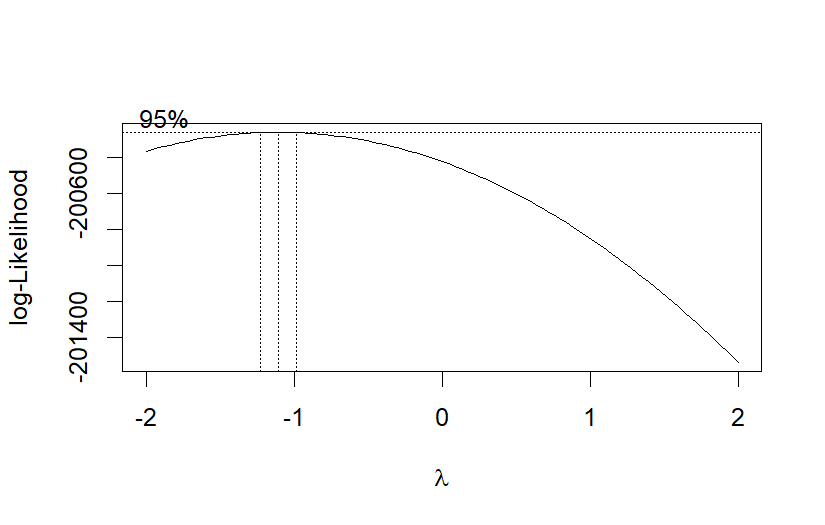
\includegraphics{qmd/appendice-chapter-6_files/figure-pdf/unnamed-chunk-5-1.png}

\legend{Source: Created by the author. See \textcite{box1964} to learn
more.}

}

\end{table}%

\begin{Shaded}
\begin{Highlighting}[numbers=left,,]
\NormalTok{lambda }\OtherTok{\textless{}{-}}\NormalTok{ box\_cox}\SpecialCharTok{$}\NormalTok{x[}\FunctionTok{which.max}\NormalTok{(box\_cox}\SpecialCharTok{$}\NormalTok{y)]}

\NormalTok{lambda}
\CommentTok{\#\textgreater{} [1] {-}1.1111}
\end{Highlighting}
\end{Shaded}

\begin{Shaded}
\begin{Highlighting}[numbers=left,,]
\NormalTok{res\_model }\OtherTok{\textless{}{-}}\NormalTok{ stats}\SpecialCharTok{::}\FunctionTok{lm}\NormalTok{(}
\NormalTok{  ((msf\_sc}\SpecialCharTok{\^{}}\NormalTok{lambda }\SpecialCharTok{{-}} \DecValTok{1}\NormalTok{) }\SpecialCharTok{/}\NormalTok{ lambda) }\SpecialCharTok{\textasciitilde{}}\NormalTok{ age }\SpecialCharTok{+}\NormalTok{ sex, }\AttributeTok{data =}\NormalTok{ data}
\NormalTok{)}
\end{Highlighting}
\end{Shaded}

\begin{Shaded}
\begin{Highlighting}[numbers=left,,]
\NormalTok{broom}\SpecialCharTok{::}\FunctionTok{tidy}\NormalTok{(res\_model)}
\end{Highlighting}
\end{Shaded}

\begin{table}

\caption{\label{tbl-appendice-chapter-6-restricted-model-summary-stats-1}Summarized
information about the components of the restricted model.}

\centering{

\begin{longtable}[]{@{}lrrrr@{}}
\toprule\noalign{}
term & estimate & std.error & statistic & p.value \\
\midrule\noalign{}
\endhead
\bottomrule\noalign{}
\endlastfoot
(Intercept) & 0.9 & 0 & 513579298.250 & 0 \\
age & 0.0 & 0 & -65.128 & 0 \\
sexMale & 0.0 & 0 & 13.020 & 0 \\
\end{longtable}

\addtocounter{table}{-1}

\legend{Source: Created by the author.}

}

\end{table}%

\begin{Shaded}
\begin{Highlighting}[numbers=left,,]
\NormalTok{broom}\SpecialCharTok{::}\FunctionTok{glance}\NormalTok{(res\_model) }\SpecialCharTok{|\textgreater{}}\NormalTok{ tidyr}\SpecialCharTok{::}\FunctionTok{pivot\_longer}\NormalTok{(}\AttributeTok{cols =}\NormalTok{ dplyr}\SpecialCharTok{::}\FunctionTok{everything}\NormalTok{())}
\end{Highlighting}
\end{Shaded}

\begin{table}

\caption{\label{tbl-appendice-chapter-6-restricted-model-summary-stats-2}Summarized
statistics about the restricted model.}

\centering{

\begin{longtable}[]{@{}lr@{}}
\toprule\noalign{}
name & value \\
\midrule\noalign{}
\endhead
\bottomrule\noalign{}
\endlastfoot
r.squared & 0.05373 \\
adj.r.squared & 0.05371 \\
sigma & 0.00000 \\
statistic & 2178.87560 \\
p.value & 0.00000 \\
df & 2.00000 \\
logLik & 1106194.89709 \\
AIC & -2212381.79419 \\
BIC & -2212344.80126 \\
deviance & 0.00000 \\
df.residual & 76741.00000 \\
nobs & 76744.00000 \\
\end{longtable}

\addtocounter{table}{-1}

\legend{Source: Created by the author.}

}

\end{table}%

\begin{Shaded}
\begin{Highlighting}[numbers=left,,]
\NormalTok{res\_model }\SpecialCharTok{|\textgreater{}} \FunctionTok{summary}\NormalTok{()}
\CommentTok{\#\textgreater{} }
\CommentTok{\#\textgreater{} Call:}
\CommentTok{\#\textgreater{} stats::lm(formula = ((msf\_sc\^{}lambda {-} 1)/lambda) \textasciitilde{} age + sex, }
\CommentTok{\#\textgreater{}     data = data)}
\CommentTok{\#\textgreater{} }
\CommentTok{\#\textgreater{} Residuals:}
\CommentTok{\#\textgreater{}           Min            1Q        Median            3Q           Max }
\CommentTok{\#\textgreater{} {-}0.0000004859 {-}0.0000000911 {-}0.0000000031  0.0000000916  0.0000004204 }
\CommentTok{\#\textgreater{} }
\CommentTok{\#\textgreater{} Coefficients:}
\CommentTok{\#\textgreater{}                     Estimate       Std. Error     t value Pr(\textgreater{}|t|)    }
\CommentTok{\#\textgreater{} (Intercept)  0.8999976603602  0.0000000017524 513579298.2   \textless{}2e{-}16 ***}
\CommentTok{\#\textgreater{} age         {-}0.0000000033812  0.0000000000519       {-}65.1   \textless{}2e{-}16 ***}
\CommentTok{\#\textgreater{} sexMale      0.0000000132309  0.0000000010162        13.0   \textless{}2e{-}16 ***}
\CommentTok{\#\textgreater{} {-}{-}{-}}
\CommentTok{\#\textgreater{} Signif. codes:  0 \textquotesingle{}***\textquotesingle{} 0.001 \textquotesingle{}**\textquotesingle{} 0.01 \textquotesingle{}*\textquotesingle{} 0.05 \textquotesingle{}.\textquotesingle{} 0.1 \textquotesingle{} \textquotesingle{} 1}
\CommentTok{\#\textgreater{} }
\CommentTok{\#\textgreater{} Residual standard error: 0.000000133 on 76741 degrees of freedom}
\CommentTok{\#\textgreater{} Multiple R{-}squared:  0.0537, Adjusted R{-}squared:  0.0537 }
\CommentTok{\#\textgreater{} F{-}statistic: 2.18e+03 on 2 and 76741 DF,  p{-}value: \textless{}2e{-}16}
\end{Highlighting}
\end{Shaded}

\subsection{Residual diagnostics}\label{residual-diagnostics}

\subsubsection{Normality}\label{normality}

\begin{Shaded}
\begin{Highlighting}[numbers=left,,]
\FunctionTok{source}\NormalTok{(here}\SpecialCharTok{::}\FunctionTok{here}\NormalTok{(}\StringTok{"R/stats\_sum.R"}\NormalTok{))}
\FunctionTok{source}\NormalTok{(here}\SpecialCharTok{::}\FunctionTok{here}\NormalTok{(}\StringTok{"R/utils.R"}\NormalTok{))}

\NormalTok{res\_model }\SpecialCharTok{|\textgreater{}}
\NormalTok{  stats}\SpecialCharTok{::}\FunctionTok{residuals}\NormalTok{() }\SpecialCharTok{|\textgreater{}}
  \FunctionTok{stats\_sum}\NormalTok{(}\AttributeTok{print =} \ConstantTok{FALSE}\NormalTok{) }\SpecialCharTok{|\textgreater{}}
  \FunctionTok{list\_as\_tibble}\NormalTok{()}
\end{Highlighting}
\end{Shaded}

\begin{table}

\caption{\label{tbl-appendice-chapter-6-restricted-model-residual-diag-stats}Statistics
about the restricted model residuals.}

\centering{

\begin{longtable}[]{@{}ll@{}}
\toprule\noalign{}
name & value \\
\midrule\noalign{}
\endhead
\bottomrule\noalign{}
\endlastfoot
n & 76744 \\
n\_rm\_na & 76744 \\
n\_na & 0 \\
mean & 6.60699976667332e-23 \\
var & 0.0000000000000176852866826985 \\
sd & 0.000000132986039427823 \\
min & -0.000000485865195534305 \\
q\_1 & -0.0000000911138016567908 \\
median & -0.00000000313530324787135 \\
q\_3 & 0.000000091553820345483 \\
max & 0.000000420368932360539 \\
iqr & 0.000000182667622002274 \\
skewness & -0.0105262146639209 \\
kurtosis & 2.82813923301771 \\
\end{longtable}

\addtocounter{table}{-1}

\legend{Source: Created by the author.}

}

\end{table}%

\begin{Shaded}
\begin{Highlighting}[numbers=left,,]
\FunctionTok{source}\NormalTok{(here}\SpecialCharTok{::}\FunctionTok{here}\NormalTok{(}\StringTok{"R/normality\_sum.R"}\NormalTok{))}

\NormalTok{res\_model }\SpecialCharTok{|\textgreater{}}
\NormalTok{  stats}\SpecialCharTok{::}\FunctionTok{residuals}\NormalTok{() }\SpecialCharTok{|\textgreater{}}
  \FunctionTok{normality\_sum}\NormalTok{()}
\end{Highlighting}
\end{Shaded}

\begin{table}

\caption{\label{tbl-appendice-chapter-6-restricted-model-residual-diag-normality-tests}Normality
tests about the restricted model residuals.}

\centering{

\begin{longtable}[]{@{}lr@{}}
\toprule\noalign{}
test & p\_value \\
\midrule\noalign{}
\endhead
\bottomrule\noalign{}
\endlastfoot
Anderson-Darling & 0.00000 \\
Bonett-Seier & 0.00000 \\
Cramer-von Mises & 0.00000 \\
D'Agostino Omnibus Test & NA \\
D'Agostino Skewness Test & 0.23383 \\
D'Agostino Kurtosis Test & NA \\
Jarque--Bera & 0.00000 \\
Lilliefors (K-S) & 0.00000 \\
Pearson chi-square & 0.00000 \\
Shapiro-Francia & NA \\
Shapiro-Wilk & NA \\
\end{longtable}

\addtocounter{table}{-1}

\legend{Source: Created by the author.}

}

\end{table}%

Correlation between observed residuals and expected residuals under
normality.

\begin{Shaded}
\begin{Highlighting}[numbers=left,,]
\NormalTok{res\_model }\SpecialCharTok{|\textgreater{}}\NormalTok{ olsrr}\SpecialCharTok{::}\FunctionTok{ols\_test\_correlation}\NormalTok{()}
\CommentTok{\#\textgreater{} [1] 0.99929}
\end{Highlighting}
\end{Shaded}

\begin{Shaded}
\begin{Highlighting}[numbers=left,,]
\FunctionTok{source}\NormalTok{(here}\SpecialCharTok{::}\FunctionTok{here}\NormalTok{(}\StringTok{"R/test\_normality.R"}\NormalTok{))}

\CommentTok{\# res\_model |\textgreater{} olsrr::ols\_plot\_resid\_qq()}

\NormalTok{qq\_plot }\OtherTok{\textless{}{-}}\NormalTok{ res\_model }\SpecialCharTok{|\textgreater{}} 
\NormalTok{  stats}\SpecialCharTok{::}\FunctionTok{residuals}\NormalTok{() }\SpecialCharTok{|\textgreater{}}
  \FunctionTok{plot\_qq}\NormalTok{(}\AttributeTok{print =} \ConstantTok{FALSE}\NormalTok{)}

\NormalTok{hist\_plot }\OtherTok{\textless{}{-}}\NormalTok{ res\_model }\SpecialCharTok{|\textgreater{}}
\NormalTok{  stats}\SpecialCharTok{::}\FunctionTok{residuals}\NormalTok{() }\SpecialCharTok{|\textgreater{}}
  \FunctionTok{plot\_hist}\NormalTok{(}\AttributeTok{print =} \ConstantTok{FALSE}\NormalTok{)}

\NormalTok{cowplot}\SpecialCharTok{::}\FunctionTok{plot\_grid}\NormalTok{(hist\_plot, qq\_plot, }\AttributeTok{ncol =} \DecValTok{2}\NormalTok{, }\AttributeTok{nrow =} \DecValTok{1}\NormalTok{)}
\end{Highlighting}
\end{Shaded}

\begin{figure}[H]

\caption{\label{fig-appendice-chapter-6-restricted-model-residual-correlation}Histogram
of the restricted model residuals with a kernel density estimate, along
with a quantile-quantile (Q-Q) plot between the residuals and the
theoretical quantiles of the normal distribution.}

\centering{

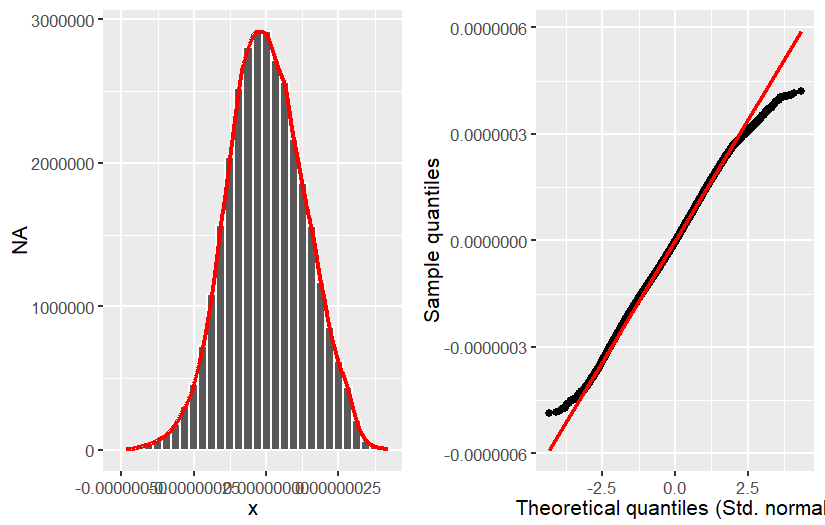
\includegraphics{qmd/appendice-chapter-6_files/figure-pdf/unnamed-chunk-14-1.png}

\legend{Source: Created by the author.}

}

\end{figure}%

\subsubsection{Common variance}\label{common-variance}

\begin{Shaded}
\begin{Highlighting}[numbers=left,,]
\NormalTok{res\_model }\SpecialCharTok{|\textgreater{}}\NormalTok{ olsrr}\SpecialCharTok{::}\FunctionTok{ols\_plot\_resid\_fit}\NormalTok{()}
\end{Highlighting}
\end{Shaded}

\begin{figure}[H]

\caption{\label{fig-appendice-chapter-6-restricted-model-residual-fit-values}Relation
between the fitted values of the restricted model and its residuals.}

\centering{

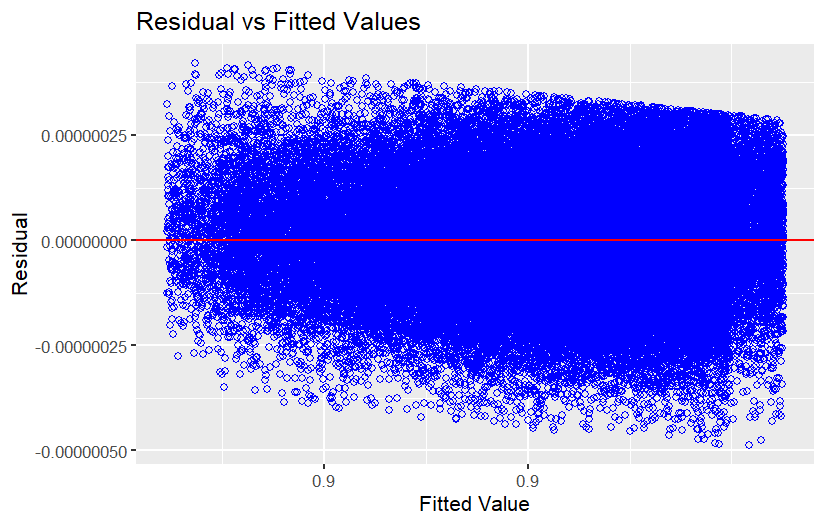
\includegraphics{qmd/appendice-chapter-6_files/figure-pdf/unnamed-chunk-15-1.png}

\legend{Source: Created by the author.}

}

\end{figure}%

\begin{Shaded}
\begin{Highlighting}[numbers=left,,]
\NormalTok{res\_model }\SpecialCharTok{|\textgreater{}} \FunctionTok{plot}\NormalTok{(}\DecValTok{3}\NormalTok{)}
\end{Highlighting}
\end{Shaded}

\begin{figure}[H]

\caption{\label{fig-appendice-chapter-6-restricted-model-residual-fit-values}Relation
between the fitted values of the restricted model and its standardized
residuals.}

\centering{

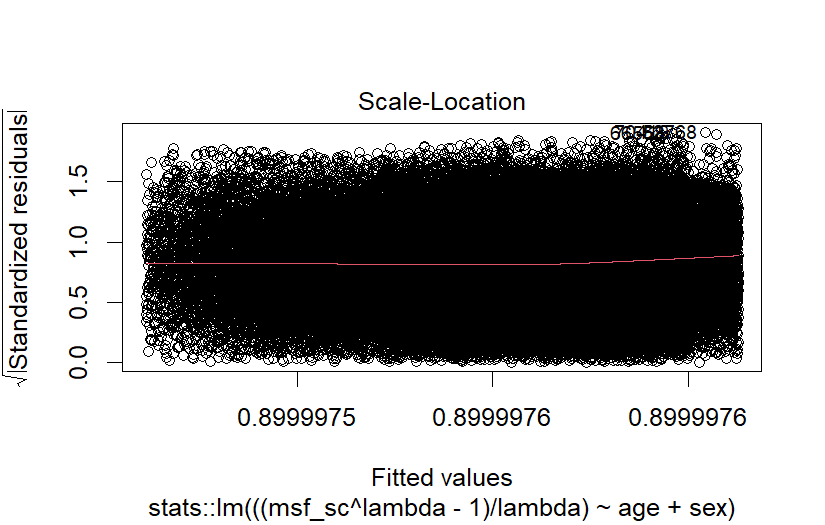
\includegraphics{qmd/appendice-chapter-6_files/figure-pdf/unnamed-chunk-16-1.png}

\legend{Source: Created by the author.}

}

\end{figure}%

\begin{Shaded}
\begin{Highlighting}[numbers=left,,]
\NormalTok{res\_model }\SpecialCharTok{|\textgreater{}}\NormalTok{ olsrr}\SpecialCharTok{::}\FunctionTok{ols\_test\_breusch\_pagan}\NormalTok{()}
\CommentTok{\#\textgreater{} }
\CommentTok{\#\textgreater{}  Breusch Pagan Test for Heteroskedasticity}
\CommentTok{\#\textgreater{}  {-}{-}{-}{-}{-}{-}{-}{-}{-}{-}{-}{-}{-}{-}{-}{-}{-}{-}{-}{-}{-}{-}{-}{-}{-}{-}{-}{-}{-}{-}{-}{-}{-}{-}{-}{-}{-}{-}{-}{-}{-}}
\CommentTok{\#\textgreater{}  Ho: the variance is constant            }
\CommentTok{\#\textgreater{}  Ha: the variance is not constant        }
\CommentTok{\#\textgreater{} }
\CommentTok{\#\textgreater{}                           Data                           }
\CommentTok{\#\textgreater{}  {-}{-}{-}{-}{-}{-}{-}{-}{-}{-}{-}{-}{-}{-}{-}{-}{-}{-}{-}{-}{-}{-}{-}{-}{-}{-}{-}{-}{-}{-}{-}{-}{-}{-}{-}{-}{-}{-}{-}{-}{-}{-}{-}{-}{-}{-}{-}{-}{-}{-}{-}{-}{-}{-}{-}{-}}
\CommentTok{\#\textgreater{}  Response : ((msf\_sc\^{}lambda {-} 1)/lambda) }
\CommentTok{\#\textgreater{}  Variables: fitted values of ((msf\_sc\^{}lambda {-} 1)/lambda) }
\CommentTok{\#\textgreater{} }
\CommentTok{\#\textgreater{}         Test Summary          }
\CommentTok{\#\textgreater{}  {-}{-}{-}{-}{-}{-}{-}{-}{-}{-}{-}{-}{-}{-}{-}{-}{-}{-}{-}{-}{-}{-}{-}{-}{-}{-}{-}{-}{-}}
\CommentTok{\#\textgreater{}  DF            =    1 }
\CommentTok{\#\textgreater{}  Chi2          =    70149.3586 }
\CommentTok{\#\textgreater{}  Prob \textgreater{} Chi2   =    0.0000}
\end{Highlighting}
\end{Shaded}

\begin{Shaded}
\begin{Highlighting}[numbers=left,,]
\NormalTok{res\_model }\SpecialCharTok{|\textgreater{}}\NormalTok{ olsrr}\SpecialCharTok{::}\FunctionTok{ols\_test\_score}\NormalTok{()}
\CommentTok{\#\textgreater{} }
\CommentTok{\#\textgreater{}  Score Test for Heteroskedasticity}
\CommentTok{\#\textgreater{}  {-}{-}{-}{-}{-}{-}{-}{-}{-}{-}{-}{-}{-}{-}{-}{-}{-}{-}{-}{-}{-}{-}{-}{-}{-}{-}{-}{-}{-}{-}{-}{-}{-}}
\CommentTok{\#\textgreater{}  Ho: Variance is homogenous}
\CommentTok{\#\textgreater{}  Ha: Variance is not homogenous}
\CommentTok{\#\textgreater{} }
\CommentTok{\#\textgreater{}  Variables: fitted values of ((msf\_sc\^{}lambda {-} 1)/lambda) }
\CommentTok{\#\textgreater{} }
\CommentTok{\#\textgreater{}       Test Summary       }
\CommentTok{\#\textgreater{}  {-}{-}{-}{-}{-}{-}{-}{-}{-}{-}{-}{-}{-}{-}{-}{-}{-}{-}{-}{-}{-}{-}{-}{-}}
\CommentTok{\#\textgreater{}  DF            =    1 }
\CommentTok{\#\textgreater{}  Chi2          =    0.000 }
\CommentTok{\#\textgreater{}  Prob \textgreater{} Chi2   =    1.000}
\end{Highlighting}
\end{Shaded}

\subsubsection{Independence}\label{independence}

\begin{description}
\item[Variance inflation factor (VIF)]
\hspace{20cm}

``Indicator of the effect that the other independent variables have on
the standard error of a regression coefficient. The variance inflation
factor is directly related to the tolerance value
(\(\text{VIF}_{i} = 1/\text{TO}L\)). Large VIF values also indicate a
high degree of collinearity or multicollinearity among the independent
variables'' \autocite[p.~265]{hair2019}.
\end{description}

\begin{Shaded}
\begin{Highlighting}[numbers=left,,]
\NormalTok{res\_model }\SpecialCharTok{|\textgreater{}}\NormalTok{ olsrr}\SpecialCharTok{::}\FunctionTok{ols\_coll\_diag}\NormalTok{()}
\CommentTok{\#\textgreater{} Tolerance and Variance Inflation Factor}
\CommentTok{\#\textgreater{} {-}{-}{-}{-}{-}{-}{-}{-}{-}{-}{-}{-}{-}{-}{-}{-}{-}{-}{-}{-}{-}{-}{-}{-}{-}{-}{-}{-}{-}{-}{-}{-}{-}{-}{-}{-}{-}{-}{-}}
\CommentTok{\#\textgreater{}   Variables Tolerance    VIF}
\CommentTok{\#\textgreater{} 1       age    0.9988 1.0012}
\CommentTok{\#\textgreater{} 2   sexMale    0.9988 1.0012}
\CommentTok{\#\textgreater{} }
\CommentTok{\#\textgreater{} }
\CommentTok{\#\textgreater{} Eigenvalue and Condition Index}
\CommentTok{\#\textgreater{} {-}{-}{-}{-}{-}{-}{-}{-}{-}{-}{-}{-}{-}{-}{-}{-}{-}{-}{-}{-}{-}{-}{-}{-}{-}{-}{-}{-}{-}{-}}
\CommentTok{\#\textgreater{}   Eigenvalue Condition Index intercept      age   sexMale}
\CommentTok{\#\textgreater{} 1   2.422418          1.0000  0.011753 0.011936 0.0669897}
\CommentTok{\#\textgreater{} 2   0.538450          2.1211  0.015824 0.018848 0.9280439}
\CommentTok{\#\textgreater{} 3   0.039132          7.8679  0.972423 0.969216 0.0049664}
\end{Highlighting}
\end{Shaded}

\subsubsection{Measures of influence}\label{measures-of-influence}

\begin{description}
\item[Leverage points]
\hspace{20cm}

``Type of \emph{influential observation} defined by one aspect of
influence termed \emph{leverage}. These observations are substantially
different on one or more independent variables, so that they affect the
estimation of one or more \emph{regression coefficients}''
\autocite[p.~262]{hair2019}.
\end{description}

\begin{Shaded}
\begin{Highlighting}[numbers=left,,]
\NormalTok{res\_model }\SpecialCharTok{|\textgreater{}}\NormalTok{ olsrr}\SpecialCharTok{::}\FunctionTok{ols\_plot\_resid\_lev}\NormalTok{()}
\end{Highlighting}
\end{Shaded}

\begin{figure}[H]

\caption{\label{fig-appendice-chapter-6-restricted-model-residual-fit-values}Relation
between the restricted model studentized residuals and their
leverage/influence.}

\centering{

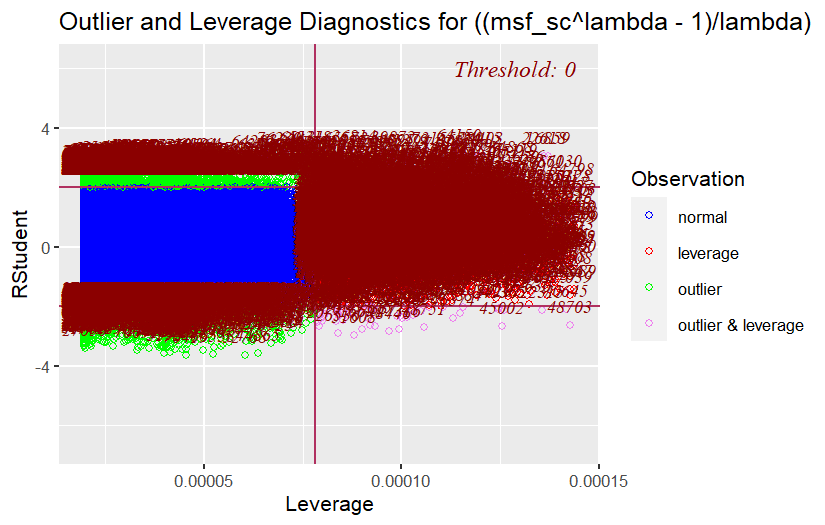
\includegraphics{qmd/appendice-chapter-6_files/figure-pdf/unnamed-chunk-20-1.png}

\legend{Source: Created by the author.}

}

\end{figure}%

\section{Full model}\label{full-model}

\subsection{Model building}\label{model-building-1}

\begin{Shaded}
\begin{Highlighting}[numbers=left,,]
\NormalTok{box\_cox }\OtherTok{\textless{}{-}}\NormalTok{ MASS}\SpecialCharTok{::}\FunctionTok{boxcox}\NormalTok{(}
\NormalTok{  msf\_sc }\SpecialCharTok{\textasciitilde{}}\NormalTok{ age }\SpecialCharTok{+}\NormalTok{ sex }\SpecialCharTok{+}\NormalTok{ latitude, }\AttributeTok{data =}\NormalTok{ data}
\NormalTok{  )}
\end{Highlighting}
\end{Shaded}

\begin{table}

\caption{\label{tbl-appendice-chapter-6-full-model-box-cox}Profile of
log-likelihoods for the parameter (\(\lambda\)) of the Box-Cox power
transformation for the full model.}

\centering{

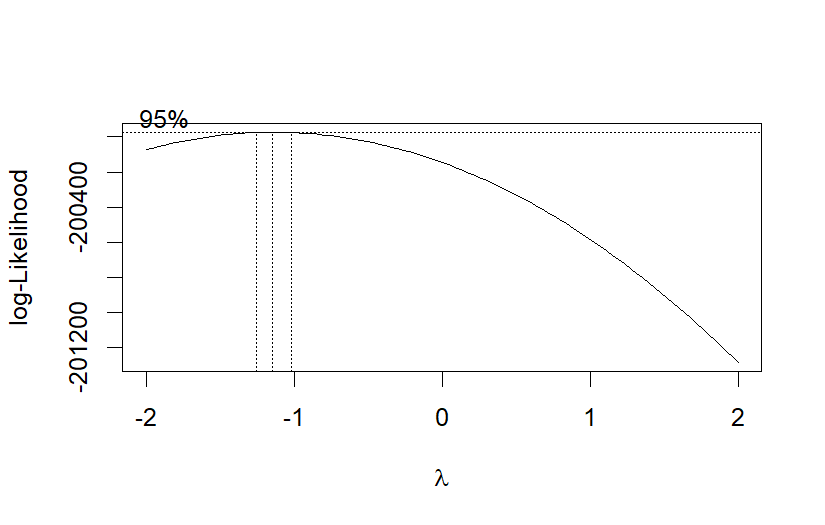
\includegraphics{qmd/appendice-chapter-6_files/figure-pdf/unnamed-chunk-21-1.png}

\legend{Source: Created by the author. See \textcite{box1964} to learn
more.}

}

\end{table}%

\begin{Shaded}
\begin{Highlighting}[numbers=left,,]
\NormalTok{box\_cox}\SpecialCharTok{$}\NormalTok{x[}\FunctionTok{which.max}\NormalTok{(box\_cox}\SpecialCharTok{$}\NormalTok{y)] }\CommentTok{\# lambda}
\CommentTok{\#\textgreater{} [1] {-}1.1515}
\end{Highlighting}
\end{Shaded}

\begin{Shaded}
\begin{Highlighting}[numbers=left,,]
\NormalTok{lambda }\CommentTok{\# The same lambda of the restricted model}
\CommentTok{\#\textgreater{} [1] {-}1.1111}
\end{Highlighting}
\end{Shaded}

\begin{Shaded}
\begin{Highlighting}[numbers=left,,]
\NormalTok{full\_model }\OtherTok{\textless{}{-}}\NormalTok{ stats}\SpecialCharTok{::}\FunctionTok{lm}\NormalTok{(}
\NormalTok{  ((msf\_sc}\SpecialCharTok{\^{}}\NormalTok{lambda }\SpecialCharTok{{-}} \DecValTok{1}\NormalTok{) }\SpecialCharTok{/}\NormalTok{ lambda) }\SpecialCharTok{\textasciitilde{}}\NormalTok{ age }\SpecialCharTok{+}\NormalTok{ sex }\SpecialCharTok{+}\NormalTok{ latitude, }
  \AttributeTok{data =}\NormalTok{ data}
\NormalTok{  )}
\end{Highlighting}
\end{Shaded}

\begin{Shaded}
\begin{Highlighting}[numbers=left,,]
\NormalTok{broom}\SpecialCharTok{::}\FunctionTok{tidy}\NormalTok{(full\_model)}
\end{Highlighting}
\end{Shaded}

\begin{table}

\caption{\label{tbl-appendice-chapter-6-full-model-summary-stats-1}Summarized
information about the components of the full model.}

\centering{

\begin{longtable}[]{@{}lrrrr@{}}
\toprule\noalign{}
term & estimate & std.error & statistic & p.value \\
\midrule\noalign{}
\endhead
\bottomrule\noalign{}
\endlastfoot
(Intercept) & 0.9 & 0 & 391908052.847 & 0 \\
age & 0.0 & 0 & -66.928 & 0 \\
sexMale & 0.0 & 0 & 13.558 & 0 \\
latitude & 0.0 & 0 & -23.852 & 0 \\
\end{longtable}

\addtocounter{table}{-1}

\legend{Source: Created by the author.}

}

\end{table}%

\begin{Shaded}
\begin{Highlighting}[numbers=left,,]
\NormalTok{broom}\SpecialCharTok{::}\FunctionTok{glance}\NormalTok{(full\_model) }\SpecialCharTok{|\textgreater{}}
\NormalTok{  tidyr}\SpecialCharTok{::}\FunctionTok{pivot\_longer}\NormalTok{(}\AttributeTok{cols =}\NormalTok{ dplyr}\SpecialCharTok{::}\FunctionTok{everything}\NormalTok{())}
\end{Highlighting}
\end{Shaded}

\begin{table}

\caption{\label{tbl-appendice-chapter-6-restricted-model-summary-stats-2}Summarized
statistics about the full model.}

\centering{

\begin{longtable}[]{@{}lr@{}}
\toprule\noalign{}
name & value \\
\midrule\noalign{}
\endhead
\bottomrule\noalign{}
\endlastfoot
r.squared & 0.06070 \\
adj.r.squared & 0.06066 \\
sigma & 0.00000 \\
statistic & 1652.97928 \\
p.value & 0.00000 \\
df & 3.00000 \\
logLik & 1106478.33068 \\
AIC & -2212946.66136 \\
BIC & -2212900.42021 \\
deviance & 0.00000 \\
df.residual & 76740.00000 \\
nobs & 76744.00000 \\
\end{longtable}

\addtocounter{table}{-1}

\legend{Source: Created by the author.}

}

\end{table}%

\begin{Shaded}
\begin{Highlighting}[numbers=left,,]
\NormalTok{full\_model }\SpecialCharTok{|\textgreater{}} \FunctionTok{summary}\NormalTok{()}
\CommentTok{\#\textgreater{} }
\CommentTok{\#\textgreater{} Call:}
\CommentTok{\#\textgreater{} stats::lm(formula = ((msf\_sc\^{}lambda {-} 1)/lambda) \textasciitilde{} age + sex + }
\CommentTok{\#\textgreater{}     latitude, data = data)}
\CommentTok{\#\textgreater{} }
\CommentTok{\#\textgreater{} Residuals:}
\CommentTok{\#\textgreater{}           Min            1Q        Median            3Q           Max }
\CommentTok{\#\textgreater{} {-}0.0000004874 {-}0.0000000911 {-}0.0000000034  0.0000000912  0.0000004328 }
\CommentTok{\#\textgreater{} }
\CommentTok{\#\textgreater{} Coefficients:}
\CommentTok{\#\textgreater{}                     Estimate       Std. Error     t value Pr(\textgreater{}|t|)    }
\CommentTok{\#\textgreater{} (Intercept)  0.8999976247783  0.0000000022965 391908052.9   \textless{}2e{-}16 ***}
\CommentTok{\#\textgreater{} age         {-}0.0000000034710  0.0000000000519       {-}66.9   \textless{}2e{-}16 ***}
\CommentTok{\#\textgreater{} sexMale      0.0000000137296  0.0000000010127        13.6   \textless{}2e{-}16 ***}
\CommentTok{\#\textgreater{} latitude    {-}0.0000000018222  0.0000000000764       {-}23.9   \textless{}2e{-}16 ***}
\CommentTok{\#\textgreater{} {-}{-}{-}}
\CommentTok{\#\textgreater{} Signif. codes:  0 \textquotesingle{}***\textquotesingle{} 0.001 \textquotesingle{}**\textquotesingle{} 0.01 \textquotesingle{}*\textquotesingle{} 0.05 \textquotesingle{}.\textquotesingle{} 0.1 \textquotesingle{} \textquotesingle{} 1}
\CommentTok{\#\textgreater{} }
\CommentTok{\#\textgreater{} Residual standard error: 0.000000132 on 76740 degrees of freedom}
\CommentTok{\#\textgreater{} Multiple R{-}squared:  0.0607, Adjusted R{-}squared:  0.0607 }
\CommentTok{\#\textgreater{} F{-}statistic: 1.65e+03 on 3 and 76740 DF,  p{-}value: \textless{}2e{-}16}
\end{Highlighting}
\end{Shaded}

\subsection{Residual diagnostics}\label{residual-diagnostics-1}

\subsubsection{Normality}\label{normality-1}

\begin{Shaded}
\begin{Highlighting}[numbers=left,,]
\FunctionTok{source}\NormalTok{(here}\SpecialCharTok{::}\FunctionTok{here}\NormalTok{(}\StringTok{"R/stats\_sum.R"}\NormalTok{))}
\FunctionTok{source}\NormalTok{(here}\SpecialCharTok{::}\FunctionTok{here}\NormalTok{(}\StringTok{"R/utils.R"}\NormalTok{))}

\NormalTok{full\_model }\SpecialCharTok{|\textgreater{}}
\NormalTok{  stats}\SpecialCharTok{::}\FunctionTok{residuals}\NormalTok{() }\SpecialCharTok{|\textgreater{}}
  \FunctionTok{stats\_sum}\NormalTok{(}\AttributeTok{print =} \ConstantTok{FALSE}\NormalTok{) }\SpecialCharTok{|\textgreater{}} 
  \FunctionTok{list\_as\_tibble}\NormalTok{()}
\end{Highlighting}
\end{Shaded}

\begin{table}

\caption{\label{tbl-appendice-chapter-6-full-model-residual-diag-stats}Statistics
about the full model residuals.}

\centering{

\begin{longtable}[]{@{}ll@{}}
\toprule\noalign{}
name & value \\
\midrule\noalign{}
\endhead
\bottomrule\noalign{}
\endlastfoot
n & 76744 \\
n\_rm\_na & 76744 \\
n\_na & 0 \\
mean & 4.85272564733669e-24 \\
var & 0.0000000000000175551361304561 \\
sd & 0.00000013249579665203 \\
min & -0.000000487410752460545 \\
q\_1 & -0.0000000910649425186321 \\
median & -0.000000003374344652286 \\
q\_3 & 0.0000000911899588839585 \\
max & 0.000000432826012898983 \\
iqr & 0.000000182254901402591 \\
skewness & 0.000655994107765645 \\
kurtosis & 2.82688323293117 \\
\end{longtable}

\addtocounter{table}{-1}

\legend{Source: Created by the author.}

}

\end{table}%

\begin{Shaded}
\begin{Highlighting}[numbers=left,,]
\FunctionTok{source}\NormalTok{(here}\SpecialCharTok{::}\FunctionTok{here}\NormalTok{(}\StringTok{"R/normality\_sum.R"}\NormalTok{))}

\NormalTok{full\_model }\SpecialCharTok{|\textgreater{}}
\NormalTok{  stats}\SpecialCharTok{::}\FunctionTok{residuals}\NormalTok{() }\SpecialCharTok{|\textgreater{}}
  \FunctionTok{normality\_sum}\NormalTok{()}
\end{Highlighting}
\end{Shaded}

\begin{table}

\caption{\label{tbl-appendice-chapter-6-full-model-residual-diag-normality-tests}Normality
tests about the full model residuals.}

\centering{

\begin{longtable}[]{@{}lr@{}}
\toprule\noalign{}
test & p\_value \\
\midrule\noalign{}
\endhead
\bottomrule\noalign{}
\endlastfoot
Anderson-Darling & 0.00000 \\
Bonett-Seier & 0.00000 \\
Cramer-von Mises & 0.00000 \\
D'Agostino Omnibus Test & NA \\
D'Agostino Skewness Test & 0.94085 \\
D'Agostino Kurtosis Test & NA \\
Jarque--Bera & 0.00000 \\
Lilliefors (K-S) & 0.00000 \\
Pearson chi-square & 0.00000 \\
Shapiro-Francia & NA \\
Shapiro-Wilk & NA \\
\end{longtable}

\addtocounter{table}{-1}

\legend{Source: Created by the author.}

}

\end{table}%

Correlation between observed residuals and expected residuals under
normality.

\begin{Shaded}
\begin{Highlighting}[numbers=left,,]
\NormalTok{full\_model }\SpecialCharTok{|\textgreater{}}\NormalTok{ olsrr}\SpecialCharTok{::}\FunctionTok{ols\_test\_correlation}\NormalTok{()}
\CommentTok{\#\textgreater{} [1] 0.99929}
\end{Highlighting}
\end{Shaded}

\begin{Shaded}
\begin{Highlighting}[numbers=left,,]
\FunctionTok{source}\NormalTok{(here}\SpecialCharTok{::}\FunctionTok{here}\NormalTok{(}\StringTok{"R/test\_normality.R"}\NormalTok{))}

\NormalTok{hist\_plot }\OtherTok{\textless{}{-}}\NormalTok{ full\_model }\SpecialCharTok{|\textgreater{}}
\NormalTok{  stats}\SpecialCharTok{::}\FunctionTok{residuals}\NormalTok{() }\SpecialCharTok{|\textgreater{}}
  \FunctionTok{plot\_hist}\NormalTok{(}\AttributeTok{print =} \ConstantTok{FALSE}\NormalTok{)}

\NormalTok{qq\_plot }\OtherTok{\textless{}{-}}\NormalTok{ full\_model }\SpecialCharTok{|\textgreater{}} 
\NormalTok{  stats}\SpecialCharTok{::}\FunctionTok{residuals}\NormalTok{() }\SpecialCharTok{|\textgreater{}}
  \FunctionTok{plot\_qq}\NormalTok{(}\AttributeTok{print =} \ConstantTok{FALSE}\NormalTok{)}

\NormalTok{cowplot}\SpecialCharTok{::}\FunctionTok{plot\_grid}\NormalTok{(hist\_plot, qq\_plot, }\AttributeTok{ncol =} \DecValTok{2}\NormalTok{, }\AttributeTok{nrow =} \DecValTok{1}\NormalTok{)}
\end{Highlighting}
\end{Shaded}

\begin{figure}[H]

\caption{\label{fig-appendice-chapter-6-restricted-model-residual-correlation}Histogram
of the full model residuals with a kernel density estimate, along with a
quantile-quantile (Q-Q) plot between the residuals and the theoretical
quantiles of the normal distribution.}

\centering{

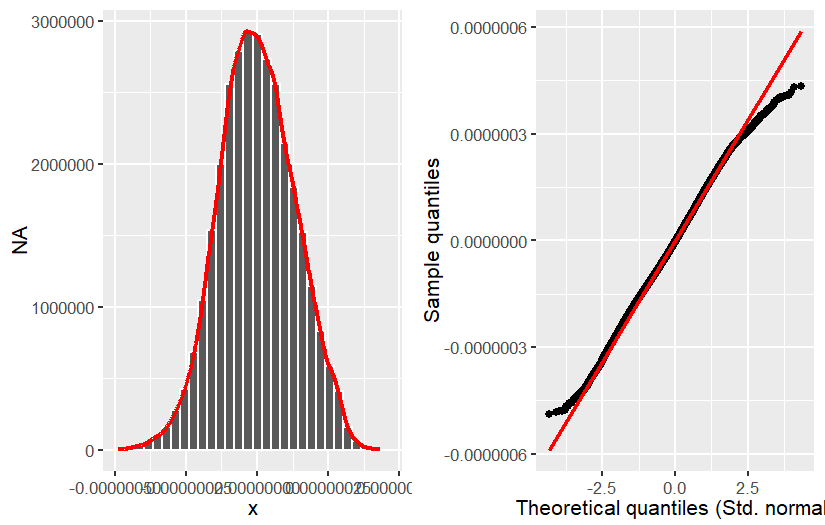
\includegraphics{qmd/appendice-chapter-6_files/figure-pdf/unnamed-chunk-31-1.png}

\legend{Source: Created by the author.}

}

\end{figure}%

\subsubsection{Common variance}\label{common-variance-1}

\begin{Shaded}
\begin{Highlighting}[numbers=left,,]
\NormalTok{full\_model }\SpecialCharTok{|\textgreater{}}\NormalTok{ olsrr}\SpecialCharTok{::}\FunctionTok{ols\_plot\_resid\_fit}\NormalTok{()}
\end{Highlighting}
\end{Shaded}

\begin{figure}[H]

\caption{\label{fig-appendice-chapter-6-restricted-model-residual-fit-values}Relation
between the fitted values of the full model and its residuals.}

\centering{

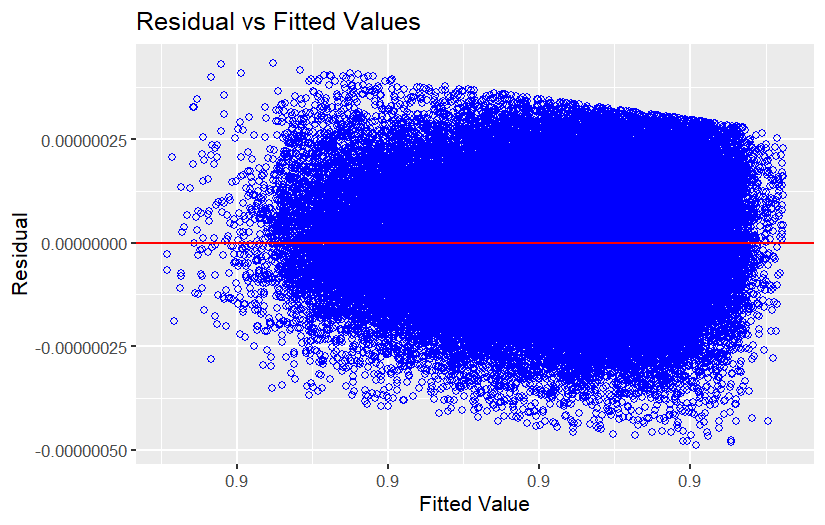
\includegraphics{qmd/appendice-chapter-6_files/figure-pdf/unnamed-chunk-32-1.png}

\legend{Source: Created by the author.}

}

\end{figure}%

\begin{Shaded}
\begin{Highlighting}[numbers=left,,]
\NormalTok{full\_model }\SpecialCharTok{|\textgreater{}} \FunctionTok{plot}\NormalTok{(}\DecValTok{3}\NormalTok{)}
\end{Highlighting}
\end{Shaded}

\begin{figure}[H]

\caption{\label{fig-appendice-chapter-6-restricted-model-residual-fit-values}Relation
between the fitted values of the full model and its standardized
residuals.}

\centering{

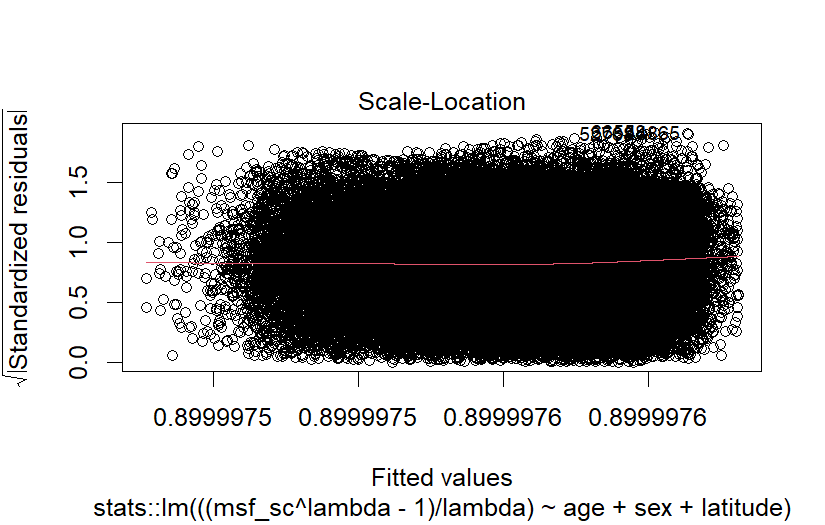
\includegraphics{qmd/appendice-chapter-6_files/figure-pdf/unnamed-chunk-33-1.png}

\legend{Source: Created by the author.}

}

\end{figure}%

\begin{Shaded}
\begin{Highlighting}[numbers=left,,]
\NormalTok{full\_model }\SpecialCharTok{|\textgreater{}}\NormalTok{ olsrr}\SpecialCharTok{::}\FunctionTok{ols\_test\_breusch\_pagan}\NormalTok{()}
\CommentTok{\#\textgreater{} }
\CommentTok{\#\textgreater{}  Breusch Pagan Test for Heteroskedasticity}
\CommentTok{\#\textgreater{}  {-}{-}{-}{-}{-}{-}{-}{-}{-}{-}{-}{-}{-}{-}{-}{-}{-}{-}{-}{-}{-}{-}{-}{-}{-}{-}{-}{-}{-}{-}{-}{-}{-}{-}{-}{-}{-}{-}{-}{-}{-}}
\CommentTok{\#\textgreater{}  Ho: the variance is constant            }
\CommentTok{\#\textgreater{}  Ha: the variance is not constant        }
\CommentTok{\#\textgreater{} }
\CommentTok{\#\textgreater{}                           Data                           }
\CommentTok{\#\textgreater{}  {-}{-}{-}{-}{-}{-}{-}{-}{-}{-}{-}{-}{-}{-}{-}{-}{-}{-}{-}{-}{-}{-}{-}{-}{-}{-}{-}{-}{-}{-}{-}{-}{-}{-}{-}{-}{-}{-}{-}{-}{-}{-}{-}{-}{-}{-}{-}{-}{-}{-}{-}{-}{-}{-}{-}{-}}
\CommentTok{\#\textgreater{}  Response : ((msf\_sc\^{}lambda {-} 1)/lambda) }
\CommentTok{\#\textgreater{}  Variables: fitted values of ((msf\_sc\^{}lambda {-} 1)/lambda) }
\CommentTok{\#\textgreater{} }
\CommentTok{\#\textgreater{}         Test Summary          }
\CommentTok{\#\textgreater{}  {-}{-}{-}{-}{-}{-}{-}{-}{-}{-}{-}{-}{-}{-}{-}{-}{-}{-}{-}{-}{-}{-}{-}{-}{-}{-}{-}{-}{-}}
\CommentTok{\#\textgreater{}  DF            =    1 }
\CommentTok{\#\textgreater{}  Chi2          =    70101.1634 }
\CommentTok{\#\textgreater{}  Prob \textgreater{} Chi2   =    0.0000}
\end{Highlighting}
\end{Shaded}

\begin{Shaded}
\begin{Highlighting}[numbers=left,,]
\NormalTok{full\_model }\SpecialCharTok{|\textgreater{}}\NormalTok{ olsrr}\SpecialCharTok{::}\FunctionTok{ols\_test\_score}\NormalTok{()}
\CommentTok{\#\textgreater{} }
\CommentTok{\#\textgreater{}  Score Test for Heteroskedasticity}
\CommentTok{\#\textgreater{}  {-}{-}{-}{-}{-}{-}{-}{-}{-}{-}{-}{-}{-}{-}{-}{-}{-}{-}{-}{-}{-}{-}{-}{-}{-}{-}{-}{-}{-}{-}{-}{-}{-}}
\CommentTok{\#\textgreater{}  Ho: Variance is homogenous}
\CommentTok{\#\textgreater{}  Ha: Variance is not homogenous}
\CommentTok{\#\textgreater{} }
\CommentTok{\#\textgreater{}  Variables: fitted values of ((msf\_sc\^{}lambda {-} 1)/lambda) }
\CommentTok{\#\textgreater{} }
\CommentTok{\#\textgreater{}       Test Summary       }
\CommentTok{\#\textgreater{}  {-}{-}{-}{-}{-}{-}{-}{-}{-}{-}{-}{-}{-}{-}{-}{-}{-}{-}{-}{-}{-}{-}{-}{-}}
\CommentTok{\#\textgreater{}  DF            =    1 }
\CommentTok{\#\textgreater{}  Chi2          =    0.000 }
\CommentTok{\#\textgreater{}  Prob \textgreater{} Chi2   =    1.000}
\end{Highlighting}
\end{Shaded}

\subsubsection{Independence}\label{independence-1}

\begin{description}
\item[Variance inflation factor (VIF)]
\hspace{20cm}

``Indicator of the effect that the other independent variables have on
the standard error of a regression coefficient. The variance inflation
factor is directly related to the tolerance value
(\(\text{VIF}_{i} = 1/\text{TO}L\)). Large VIF values also indicate a
high degree of collinearity or multicollinearity among the independent
variables'' \autocite[p.~265]{hair2019}.
\end{description}

\begin{Shaded}
\begin{Highlighting}[numbers=left,,]
\NormalTok{full\_model }\SpecialCharTok{|\textgreater{}}\NormalTok{ olsrr}\SpecialCharTok{::}\FunctionTok{ols\_coll\_diag}\NormalTok{()}
\CommentTok{\#\textgreater{} Tolerance and Variance Inflation Factor}
\CommentTok{\#\textgreater{} {-}{-}{-}{-}{-}{-}{-}{-}{-}{-}{-}{-}{-}{-}{-}{-}{-}{-}{-}{-}{-}{-}{-}{-}{-}{-}{-}{-}{-}{-}{-}{-}{-}{-}{-}{-}{-}{-}{-}}
\CommentTok{\#\textgreater{}   Variables Tolerance    VIF}
\CommentTok{\#\textgreater{} 1       age   0.99354 1.0065}
\CommentTok{\#\textgreater{} 2   sexMale   0.99838 1.0016}
\CommentTok{\#\textgreater{} 3  latitude   0.99441 1.0056}
\CommentTok{\#\textgreater{} }
\CommentTok{\#\textgreater{} }
\CommentTok{\#\textgreater{} Eigenvalue and Condition Index}
\CommentTok{\#\textgreater{} {-}{-}{-}{-}{-}{-}{-}{-}{-}{-}{-}{-}{-}{-}{-}{-}{-}{-}{-}{-}{-}{-}{-}{-}{-}{-}{-}{-}{-}{-}}
\CommentTok{\#\textgreater{}   Eigenvalue Condition Index  intercept       age   sexMale  latitude}
\CommentTok{\#\textgreater{} 1   3.312504          1.0000 0.00377395 0.0064918 0.0304493 0.0068553}
\CommentTok{\#\textgreater{} 2   0.584652          2.3803 0.00328127 0.0064143 0.9588857 0.0083393}
\CommentTok{\#\textgreater{} 3   0.073700          6.7042 0.00040414 0.5063551 0.0023826 0.5659326}
\CommentTok{\#\textgreater{} 4   0.029145         10.6609 0.99254063 0.4807389 0.0082824 0.4188728}
\end{Highlighting}
\end{Shaded}

\subsubsection{Measures of influence}\label{measures-of-influence-1}

\begin{description}
\item[Leverage points]
\hspace{20cm}

``Type of \emph{influential observation} defined by one aspect of
influence termed \emph{leverage}. These observations are substantially
different on one or more independent variables, so that they affect the
estimation of one or more \emph{regression coefficients}''
\autocite[p.~262]{hair2019}.
\end{description}

\begin{Shaded}
\begin{Highlighting}[numbers=left,,]
\NormalTok{full\_model }\SpecialCharTok{|\textgreater{}}\NormalTok{ olsrr}\SpecialCharTok{::}\FunctionTok{ols\_plot\_resid\_lev}\NormalTok{()}
\end{Highlighting}
\end{Shaded}

\begin{figure}[H]

\caption{\label{fig-appendice-chapter-6-restricted-model-residual-fit-values}Relation
between the full model studentized residuals and their
leverage/influence.}

\centering{

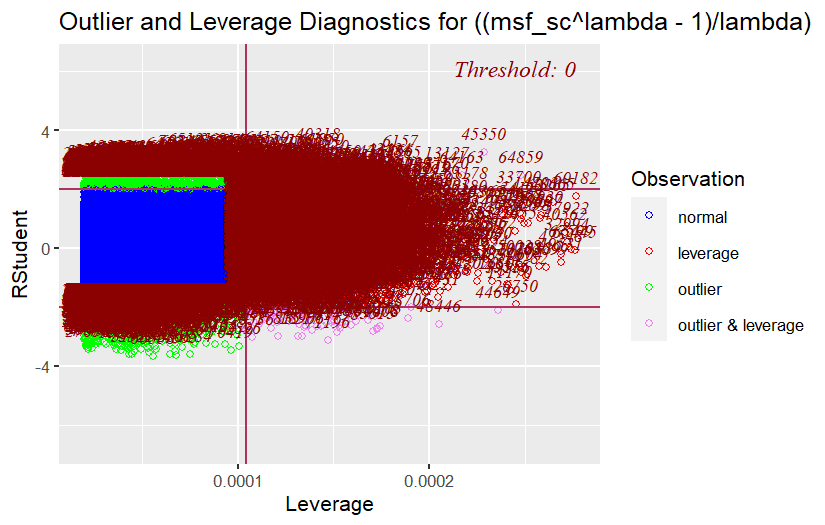
\includegraphics{qmd/appendice-chapter-6_files/figure-pdf/unnamed-chunk-37-1.png}

\legend{Source: Created by the author.}

}

\end{figure}%

\section{Hypothesis test}\label{hypothesis-test}

\[
\begin{cases}
\text{H}_{0}: \text{R}^{2}_{\text{res}} >= \text{R}^{2}_{\text{full}} \\
\text{H}_{a}: \text{R}^{2}_{\text{res}} < \text{R}^{2}_{\text{full}}
\end{cases}
\]

\[
\text{F} = \cfrac{\text{R}^{2}_{F} - \text{R}^{2}_{R} / (k_{F} - k_{R})}{(1 - \text{R}^{2}_{F}) / (\text{N} - k_{F} - 1)}
\]

\[
\text{F} = \cfrac{\text{Additional Var. Explained} / \text{Additional d.f. Expended}}{\text{Var. unexplained} / \text{d.f. Remaining}}
\]

\smallskip

\begin{Shaded}
\begin{Highlighting}[numbers=left,,]
\FunctionTok{source}\NormalTok{(here}\SpecialCharTok{::}\FunctionTok{here}\NormalTok{(}\StringTok{"R/utils{-}stats.R"}\NormalTok{))}

\NormalTok{dplyr}\SpecialCharTok{::}\FunctionTok{tibble}\NormalTok{(}
  \AttributeTok{name =} \FunctionTok{c}\NormalTok{(}\StringTok{"r\_squared\_res"}\NormalTok{, }\StringTok{"r\_squared\_full"}\NormalTok{, }\StringTok{"diff"}\NormalTok{),}
  \AttributeTok{value =} \FunctionTok{c}\NormalTok{(}
  \FunctionTok{r\_squared}\NormalTok{(res\_model), }\FunctionTok{r\_squared}\NormalTok{(full\_model), }
  \FunctionTok{r\_squared}\NormalTok{(full\_model) }\SpecialCharTok{{-}} \FunctionTok{r\_squared}\NormalTok{(res\_model)}
\NormalTok{  )}
\NormalTok{)}
\end{Highlighting}
\end{Shaded}

\begin{table}

\caption{\label{tbl-appendice-chapter-6-hypothesis-test-r-squared-comparison}Comparison
between the coefficients of determination (\(\text{R}^2\)) of the
restricted and full model.}

\centering{

\begin{longtable}[]{@{}lr@{}}
\toprule\noalign{}
name & value \\
\midrule\noalign{}
\endhead
\bottomrule\noalign{}
\endlastfoot
r\_squared\_res & 0.05373 \\
r\_squared\_full & 0.06070 \\
diff & 0.00696 \\
\end{longtable}

\addtocounter{table}{-1}

\legend{Source: Created by the author.}

}

\end{table}%

\begin{Shaded}
\begin{Highlighting}[numbers=left,,]
\FunctionTok{print}\NormalTok{(stats}\SpecialCharTok{::}\FunctionTok{anova}\NormalTok{(res\_model, full\_model))}
\CommentTok{\#\textgreater{} Analysis of Variance Table}
\CommentTok{\#\textgreater{} }
\CommentTok{\#\textgreater{} Model 1: ((msf\_sc\^{}lambda {-} 1)/lambda) \textasciitilde{} age + sex}
\CommentTok{\#\textgreater{} Model 2: ((msf\_sc\^{}lambda {-} 1)/lambda) \textasciitilde{} age + sex + latitude}
\CommentTok{\#\textgreater{}   Res.Df           RSS Df        Sum of Sq   F Pr(\textgreater{}F)    }
\CommentTok{\#\textgreater{} 1  76741 0.00000000136                                   }
\CommentTok{\#\textgreater{} 2  76740 0.00000000135  1 0.00000000000999 569 \textless{}2e{-}16 ***}
\CommentTok{\#\textgreater{} {-}{-}{-}}
\CommentTok{\#\textgreater{} Signif. codes:  0 \textquotesingle{}***\textquotesingle{} 0.001 \textquotesingle{}**\textquotesingle{} 0.01 \textquotesingle{}*\textquotesingle{} 0.05 \textquotesingle{}.\textquotesingle{} 0.1 \textquotesingle{} \textquotesingle{} 1}
\end{Highlighting}
\end{Shaded}

\begin{Shaded}
\begin{Highlighting}[numbers=left,,]
\FunctionTok{source}\NormalTok{(here}\SpecialCharTok{::}\FunctionTok{here}\NormalTok{(}\StringTok{"R/utils{-}stats.R"}\NormalTok{))}

\NormalTok{n }\OtherTok{\textless{}{-}} \FunctionTok{nrow}\NormalTok{(data)}
\NormalTok{k\_res }\OtherTok{\textless{}{-}} \FunctionTok{length}\NormalTok{(stats}\SpecialCharTok{::}\FunctionTok{coefficients}\NormalTok{(res\_model)) }\SpecialCharTok{{-}} \DecValTok{1}
\NormalTok{k\_full }\OtherTok{\textless{}{-}} \FunctionTok{length}\NormalTok{(stats}\SpecialCharTok{::}\FunctionTok{coefficients}\NormalTok{(full\_model)) }\SpecialCharTok{{-}} \DecValTok{1}

\NormalTok{((}\FunctionTok{r\_squared}\NormalTok{(full\_model) }\SpecialCharTok{{-}} \FunctionTok{r\_squared}\NormalTok{(res\_model)) }\SpecialCharTok{/}\NormalTok{ (k\_full }\SpecialCharTok{{-}}\NormalTok{ k\_res)) }\SpecialCharTok{/} 
\NormalTok{  ((}\DecValTok{1} \SpecialCharTok{{-}} \FunctionTok{r\_squared}\NormalTok{(full\_model)) }\SpecialCharTok{/}\NormalTok{ (n  }\SpecialCharTok{{-}}\NormalTok{ k\_full }\SpecialCharTok{{-}} \DecValTok{1}\NormalTok{))}
\CommentTok{\#\textgreater{} [1] 568.94}
\end{Highlighting}
\end{Shaded}

\[
f^{2} = \cfrac{\text{R}^{2}_{F} - \text{R}^{2}_{R}}{1 - \text{R}^{2}_{F}}
\]

\[
f^{2} = \cfrac{\text{Additional Var. Explained}}{\text{Var. unexplained}}
\]

\smallskip

\begin{Shaded}
\begin{Highlighting}[numbers=left,,]
\FunctionTok{source}\NormalTok{(here}\SpecialCharTok{::}\FunctionTok{here}\NormalTok{(}\StringTok{"R/cohens\_f\_squared.R"}\NormalTok{))}
\FunctionTok{source}\NormalTok{(here}\SpecialCharTok{::}\FunctionTok{here}\NormalTok{(}\StringTok{"R/utils{-}stats.R"}\NormalTok{))}

\FunctionTok{cohens\_f\_squared\_summary}\NormalTok{(}
  \FunctionTok{adj\_r\_squared}\NormalTok{(res\_model), }
  \FunctionTok{adj\_r\_squared}\NormalTok{(full\_model)}
\NormalTok{  )}
\end{Highlighting}
\end{Shaded}

\begin{table}

\caption{\label{tbl-appendice-chapter-6-hypothesis-test-r-squared-comparison}Effect
size between the restricted and full model based on Cohen's \(f^2\).}

\centering{

\begin{longtable}[]{@{}ll@{}}
\toprule\noalign{}
name & value \\
\midrule\noalign{}
\endhead
\bottomrule\noalign{}
\endlastfoot
f\_squared & 0.00740068896515648 \\
effect\_size & Negligible \\
\end{longtable}

\addtocounter{table}{-1}

\legend{Source: Created by the author. See \textcite{cohen1988};
\textcite{cohen1992} to learn more.}

}

\end{table}%

\end{apendicesenv}



\tocskipone
\tocprintchapternonum

\begingroup
\ABNTEXfontereduzida
\renewcommand{\baselinestretch}{1}
\setlength{\parindent}{0pt}
\setlength{\parskip}{\tinyskipamount}
\setlength{\afterchapskip}{\hugeskipamount}
\phantompart
\printindex
\endgroup
\end{document}
